% W A R N I N G: STAY OUT. Modify style.cls without consulting me, and you WILL answer to me. -Bryan


%\\\\\\\\\\\Document Properties\\\\\\\\\\\\\\\\\\\\\\\\\\\\\\\\\\\\\\\\\\\\\\\\\\\\\\\\\\\\\\\\\\\\\\\\\\\\\\\\\\\\\\\\\

\documentclass[11pt,a4paper,reqno,titlepage,twoside,openright]{report} %twoside,openright together forces a new chapter to begin on a right side
\raggedbottom
\usepackage[margin=6pc]{geometry}
\usepackage[utf8]{inputenc}
\usepackage{amsfonts}
\usepackage{amsmath}
\usepackage{mathtools}
\usepackage{amssymb}
\usepackage{graphicx}
\usepackage{tabularx}
\usepackage{float}
\usepackage{booktabs}
\usepackage{titlesec,color}
\usepackage{caption}
\usepackage{enumitem}
\setlist{itemsep=.5pt}%added by steph for more compact lists
\usepackage{subcaption}
\usepackage{pdfpages}
\usepackage[hyphens]{url}
\usepackage{array}
\usepackage{notoccite}
\usepackage[symbol]{footmisc}
\usepackage{listings}
\usepackage{siunitx}
\usepackage[toc, titletoc]{appendix}
\usepackage{fancyhdr} %header package
\usepackage{comment} %begincomment + endcomment package
\usepackage{tablefootnote} %footnotes within a table
\usepackage{hyperref}
\usepackage{cleveref} %reference to multiple figures at the same time: \Cref{fig1,fig2,fig3} depicts Figures 1 to 3.
\usepackage{multirow}
\usepackage{longtable}
\usepackage[table]{xcolor} %Adding colors to table cells
\usepackage{adjustbox} %Shrinking table sizes so tables can fit within in a page
\usepackage{eurosym}
\usepackage{pifont} %for checkmarks
\usepackage{arydshln} %Adding dashlines in arrays \hdashline


%\\\\\\\\\\\Document Properties\\\\\\\\\\\\\\\\\\\\\\\\\\\\\\\\\\\\\\\\\\\\\\\\\\\\\\\\\\\\\\\\\\\\\\\\\\\\\\\\\\\\\\\\

%\usepackage[hidelinks, pdftitle={High Speed Wind Tunnel Report Group 36}, pdfauthor={W. Broeders, et. al}, pdfsubject={AE2130-III Aerodynamics II}]{hyperref}

%\\\\\\\\\\\Setting-up Nomenclature Classes\\\\\\\\\\\\\\\\\\\\\\\\\\\\\\\\\\\\\\\\\\\\\\\\\\\\\\\\\\\\\\\\\\\\\\\\\\\\

\usepackage{nomencl}
\makenomenclature

\usepackage{etoolbox}
\renewcommand\nomgroup[1]{%
	\item[\bfseries
	\ifstrequal{#1}{G}{Greek Symbols}{%
		\ifstrequal{#1}{B}{Roman Symbols}{%
			%ADD MORE CLASSES HERE (Order does not matter, LaTeX will sort classes Based on !Class Reference
			%\ifstrequal{#1}{!Class Reference}{!Class Name}{%
			%\ifstrequal{#1}{!Class Reference}{!Class Name}{%
			%\ifstrequal{#1}{!Class Reference}{!Class Name}{%
			\ifstrequal{#1}{A}{Abbreviations}{}}}%
	]}

% This argument will add the units
\newcommand{\nomunit}[1]{%
	\renewcommand{\nomentryend}{\hspace*{\fill}[#1]}}

%Renames Nomenclature to List of Symbols
\renewcommand{\nomname}{List of Symbols}

%\\\\\\\\\\\Definining MATLAB Appendix Colors\\\\\\\\\\\\\\\\\\\\\\\\\\\\\\\\\\\\\\\\\\\\\\\\\\\\\\\\\\\\\\\\\\\\\\\\\\

%\definecolor{mygreen}{RGB}{28,172,0}
%\definecolor{mylilas}{RGB}{170,55,241}
%\definecolor{mygrey}{RGB}{125,125,125}
%\definecolor{myBG}{RGB}{252,252,220}

%\\\\\\\\\\Table Spacing & Layout Parameters\\\\\\\\\\\\\\\\\\\\\\\\\\\\\\\\\\\\\\\\\\\\\\\\\\\\\\\\\\\\\\\\\\\\\\\\\\\

\renewcommand{\arraystretch}{1.2}
\newcolumntype{C}{>{\small\centering\arraybackslash}X} %For tabularX
\newcolumntype{L}{>{\small\raggedright\arraybackslash}X} %For tabularX
\newcolumntype{R}{>{\small\raggedleft\arraybackslash}X} %For tabularX
\newcolumntype{P}[1]{>{\centering\arraybackslash}p{#1}} %Allows column width adjustments while maintaining center alignment

%Changes parameters for \hdashline to make the dashes into dots:
\setlength\dashlinedash{0.2pt}
\setlength\dashlinegap{1.5pt}
\setlength\arrayrulewidth{0.3pt}

%\\\\\\\\\\\Set Document Layout & Title Margins\\\\\\\\\\\\\\\\\\\\\\\\\\\\\\\\\\\\\\\\\\\\\\\\\\\\\\\\\\\\\\\\\\\\\\\\

\titlespacing*{\chapter}{0pt}{-25pt}{10pt}
\definecolor{gray75}{gray}{0}
\newcommand{\hsp}{\hspace{3pt}}
\titleformat{\chapter}[hang]{\Huge\bfseries}{\thechapter\hsp\textcolor{gray75}\hsp}{10pt}{\Huge\bfseries}
%\titlespacing*{\section}{0pt}{.4cm}{.2cm}%added by steph for title spacing
%\titlespacing*{\subsection}{0pt}{.3cm}{.1cm}%added by steph for title spacing


%\\\\\\\\\\\Rename Bibliography to References\\\\\\\\\\\\\\\\\\\\\\\\\\\\\\\\\\\\\\\\\\\\\\\\\\\\\\\\\\\\\\\\\\\\\\\\\\

\usepackage[
backend=biber,
style=numeric,
citestyle=numeric,
sorting=none
]{biblatex}
\addbibresource{references.bib} %Bibliography File
\newcommand{\BibliographyName}{References} %Name of Biblography

%\\\\\\\\\\\Putting Chapter Titles, Page Number and Line in Header Section\\\\\\\\\\\\\\\\\\\\\\\\\\\\\\\\\\\\\\\\\\\\\\\\\\\\\\\\\\\\\\\\\\\\\\\\\\

\pagestyle{fancy}
\fancyhf{}
\rhead{\thepage} %Puts a page number on the right side of a header
\lhead{\leftmark} %Puts a chapter number and name on the left side of a header
\rfoot{}
\let\MakeUppercase\relax

%\\\\\\\\\\\Changing Footnote Counts to Arabic\\\\\\\\\\\\\\\\\\\\\\\\\\\\\\\\\\\\\\\\\\\\\\\\\\\\\\\\\\\\\\\\\\\\\\\\\\

\renewcommand{\thefootnote}{\arabic{footnote}}

%\\\\\\\\\\\Putting autoref for subsections, sections and chapters in capital\\\\\\\\\\\\\\\\\\\\\\\\\\\\\\\\\\\\\\\\\\\\\\\\\\\\\\\\\\\\\\\\\\\\\\\\\\

\renewcommand{\chapterautorefname}{Chapter}
\renewcommand{\sectionautorefname}{Section}
\renewcommand{\subsectionautorefname}{Section}
\renewcommand{\subsubsectionautorefname}{Section}

%\\\\\\\\\\\Misc\\\\\\\\\\\\\\\\\\\\\\\\\\\\\\\\\\\\\\\\\\\\\\\\\\\\\\\\\\\\\\\\\\\\\\\\\\
\newcommand{\cmark}{\ding{51}}% for checkmark

%Document
\begin{document}  
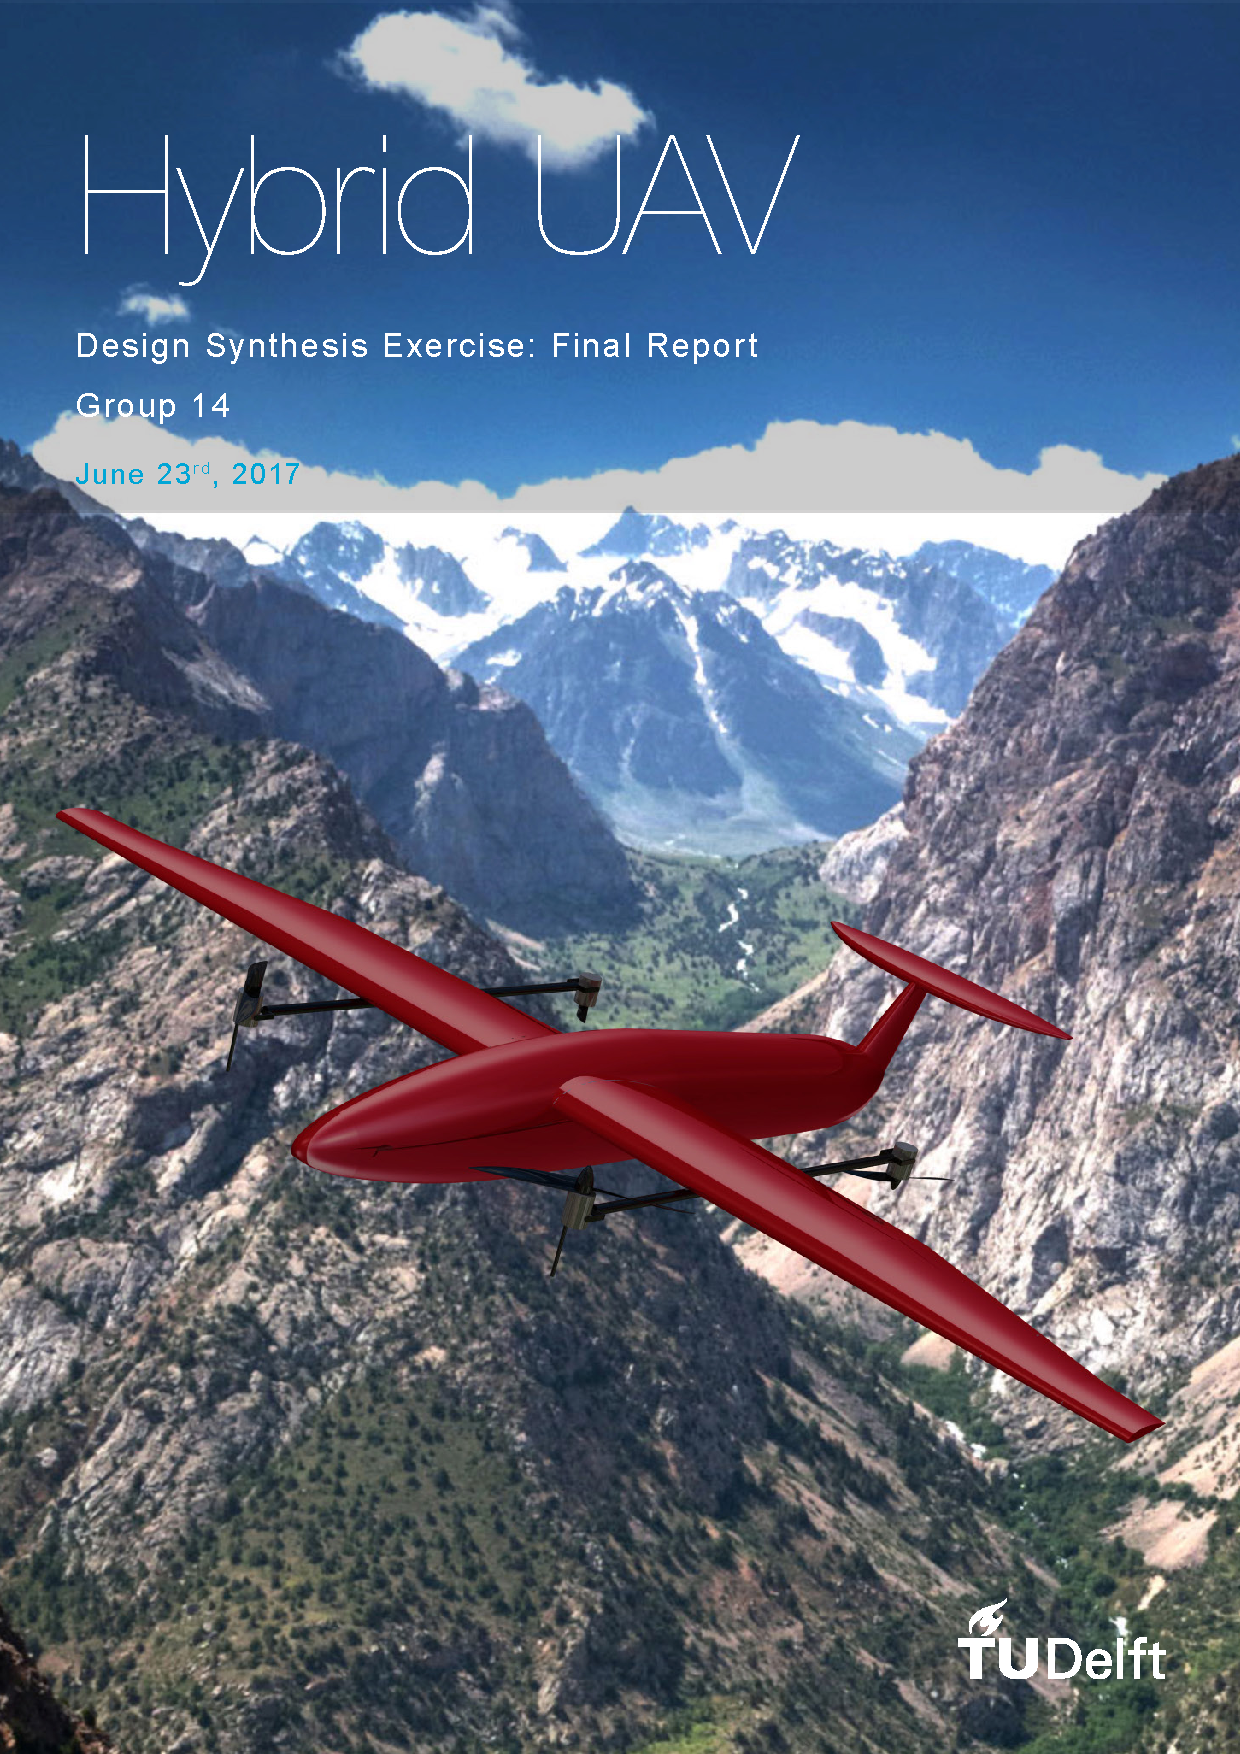
\includepdf[pages={1}]{title.pdf}
\setlength{\parindent}{0cm} % No indent

%A blank page for printed versions
\begin{titlepage}
This page is intentionally left blank.
\end{titlepage}


%Inner Title Page
\newgeometry{margin=6pc} %Change Title-Page Margin Differently
\begin{titlepage}
\begin{center}

\textsc{\LARGE Delft University of Technology}\\[1.5cm]

\includegraphics[scale=0.45]{TU_Delft_logo_RGB.png}\\[0.5cm]
\textsc{\Large AE3200 - Design Synthesis Exercise}\\[0.5cm]
{\huge\textbf{Final Report} \\[.2cm] \Large\textsc{Version 1.0}\\[1.0cm]}

\begin{minipage}[t]{0.4\textwidth}
\begin{flushleft} \large
\emph{Authors:}\\
    4384385  Jong, C.P.L. de\\
    4221699  Kim, M.\\
    4376161  Lee, J.J. van de\\
    4371321  Lovell-Prescod, G.H.\\
    4308220  Ruland, O.L.\\
    4344499  Sokolowski, P.M.\\
    4279832  Steiner, L.F.\\
    4364228  Wellens, L.\\
    4280806  Wheeler, K.\\
    4381726  Wiechers, S.M.G.
    

\end{flushleft}
\end{minipage}
\begin{minipage}[t]{0.4\textwidth}
\begin{flushright} \large
\emph{Supervisors:} \\
    Jos Sinke\\
    Sebastian Rapp\\
    Erik-Jan van Kampen
    
    
\end{flushright}
\end{minipage}
\vfill
\textit{Cover Image:} \\
\small
\url{}

\end{center}
\end{titlepage}
\restoregeometry
%A blank page for printed versions
\begin{titlepage}
This page is intentionally left blank.
\end{titlepage}



%Document Part I:
\begingroup
\pagenumbering{roman} % Roman numbering
    
    %Summary
    \chapter*{Preface}
\setlength{\parindent}{15pt}
\label{ch:pref}


    \chapter*{Summary} 
\setlength{\parindent}{15pt}
\label{ch:summ}










 % Summary
    \addcontentsline{toc}{chapter}{Preface}
    \addcontentsline{toc}{chapter}{Summary} % Adding the Summary to the ToC

    %Table of Contents
    \setcounter{tocdepth}{1}
    \renewcommand{\contentsname}{Table of Contents}
    \tableofcontents
    \thispagestyle{empty}

    \clearpage

    %List of Symbols
    \printnomenclature[50pt]
    \addcontentsline{toc}{chapter}{List of Symbols}
    \begin{titlepage}
This page is intentionally left blank.
\end{titlepage}

 %ONLY ENABLE THIS IF INTRODUCTION IS PRINTED ON THE BACK SIDE OF LIST OF SYMBOLS 

    %List of Figures
    %\listoffigures
    %\addcontentsline{toc}{chapter}{List of Figures}

    %List of Tables
    %\listoftables
    %\addcontentsline{toc}{chapter}{List of Tables}
\endgroup
\clearpage

%Document Part II:
\begingroup
\pagenumbering{arabic}

    %\chapter{SAMPLE}
\pagenumbering{arabic}

This template has been developed for the [AE3200] Design Synthesis Exercise. \texttt{THIS TEMPLATE CANNOT BE USED WITHOUT EXPRESSED PERMISSION FROM:} \c{S}an K{\i}lk{\i}\c{s} and Munyung Kim

\section{Tables \& Figures}
An example \autoref{tab:exampletable} and an example \autoref{fig:flame} can be found in this section. When you label tables or figures, make sure to use `tab:name' or `fig:name'. For inserting 2+ figures in a row, look at the formatting of Figure \autoref{fig:sbs}. Using the \texttt{autocite} command negates the need for manually typing `Table' or `Figure'. The syntax is as follows, note that the `tab' in `tab:exampletable' is not necessary for \texttt{autocite} and is purely for organizational reasons.

\begin{verbatim}
    \autoref{tab:exampletable}
\end{verbatim}

The Tables below use the package \texttt{tabularx} which adjusts column spacing automatically to fit the table within the margins of the page. The syntax is as follows where 'L' is for Left Aligned, 'C' for Centered, and 'R' is for Right Aligned. If you wish to make a long table with \textit{longtable}, an example can be seen after the \textit{tabularx} example. You can use a normal tabular environment unless you really want an equal column spacing.

\begin{verbatim}
    \begin{tabularx}{\textwidth}{L C C C}
\end{verbatim}

\begin{verbatim}
	\begin{longtable}[htb]{llccc}
	\caption{Task division of the mid-term report}\label{tab:taskdivi}\\
\end{verbatim}

For longtable, do NOT use \textit{\centering}, as longtable by default puts the table in center. In order to keep up the same appearance for all tables use the commands \texttt{toprule}, \texttt{midrule}, \texttt{bottomrule}, and \texttt{hdashline} to create the horizontal lines. NO VERTICAL LINES ARE ALLOWED!

\begin{table}[H]
	\centering
	\caption{Example Table}
	\label{tab:exampletable}
	\begin{tabularx}{\textwidth}{L C C C} %'L' for Left Aligned, 'C' for Centered, 'R' for Right Aligned
	    \toprule\
		\textbf{Component}				& \textbf{Mass [$\text{kg}$]}	&\textbf{Location [$\text{m}$]} & \textbf{Location [\% MAC]}   \\ \toprule
		Wing 							& 425.4 						& 5.74 							& 40.00\\\hdashline
		Main Landing Gear 				& 243.1 						& 5.82 							& 45.00 \\\hdashline
		Fuel System 					& 80.74 						& 5.91 							& 50.00 \\\hdashline
		Flight Control System 			& 48.61 						& 6.08 							& 60.00	\\\hdashline
		Hydraulics 						& 4.660 						& 6.08 						    & 60.00 \\\hdashline
		\textbf{Wing Group} 			& \textbf{802.5} 				& \textbf{5.80} 				& \textbf{43.85}\\ \midrule
		Fuselage 						& 265.2 						& 5.74 	                        & 40.00 \\\hdashline
		Engine 							& 409.4 						& 1.64 							& - \\\hdashline
		Avionics 						& 490.9 						& 4.39 							& - \\\hdashline
		H. Tail 						& 42.93 						& 13.2 						    & - \\\hdashline
		V. Tail 						& 66.43 						& 12.6 						    & - \\\hdashline
		Nose Gear						& 54.58 						& 2.50 							& - \\\hdashline
		Electrical 						& 217.4 						& 6.16 							& 67.12 \\\hdashline
		AC \& Anti-Ice 					& 215.7 						& 6.16 							& 67.12 \\\hdashline
		Furnishings 					& 241.5 						& 6.16 							& 67.12 \\\hdashline
		\textbf{Fuselage Group} 		& \textbf{2004} 				& \textbf{5.01} 				& \textbf{-2.32} \\ \midrule
		\textbf{OEW C.G.} 				& \textbf{2806} 				& \textbf{5.24} 				& \textbf{10.88} \\ \bottomrule
	\end{tabularx}
\end{table}

Here's how you make a long table that breaks automatically over pages (just copy this if you want to make one)
\begin{verbatim}
    \begin{longtable}[]{l l p{.3\linewidth}} %'l' is left aligned, but for pieces with text use p{size} to define column width
        \caption{Long tables are awesome\label{tab:haha_fun}}\\ %putting label below gives an error and you need the enter\\
        %now define the layout of the table
        \toprule
        This is the text that only will go at the beginning of your table (so just once)
        \\ \midrule
        \endfirsthead
        %%%%
        \caption[]{(continued)}
        \toprule
        This is something that goes on top of each part on every page the table spans
        \\ \midrule
        \endhead
        %%%%
        \midrule \endfoot
        \bottomrule \endlastfoot
        Now & this & is\\
        the & place & where\\
        the & table & goes \\
    \end{longtable}
\end{verbatim}

\begin{table}[H]
	\centering
	\caption{Example Table II}
	\label{tab:exampletableII}
    \begin{tabularx}{\textwidth}{C C C C C C C C} %'L' for Left Aligned, 'C' for Centered, 'R' for Right Aligned
    \toprule\
    {$m$} & {$\Re\{\underline{\mathfrak{X}}(m)\}$} & {$-\Im\{\underline{\mathfrak{X}}(m)\}$} & {$\mathfrak{X}(m)$} & {$\frac{\mathfrak{X}(m)}{23}$} & {$A_m$} & {$\varphi(m)\ /\ ^{\circ}$} & {$\varphi_m\ /\ ^{\circ}$} \\ \toprule
    1  & 16.128 & +8.872 & 16.128 & 1.402 & 1.373 & -146.6 & -137.6 \\ \hdashline
    2  & 3.442  & -2.509 & 3.442  & 0.299 & 0.343 & 133.2  & 152.4  \\ \hdashline
    3  & 1.826  & -0.363 & 1.826  & 0.159 & 0.119 & 168.5  & -161.1 \\ \hdashline
    4  & 0.993  & -0.429 & 0.993  & 0.086 & 0.08  & 25.6   & 90     \\ \midrule
    5  & 1.29   & +0.099 & 1.29   & 0.112 & 0.097 & -175.6 & -114.7 \\ \hdashline
    6  & 0.483  & -0.183 & 0.483  & 0.042 & 0.063 & 22.3   & 122.5  \\ \hdashline
    7  & 0.766  & -0.475 & 0.766  & 0.067 & 0.039 & 141.6  & -122   \\ \hdashline
    8  & 0.624  & +0.365 & 0.624  & 0.054 & 0.04  & -35.7  & 90     \\ \midrule
    9  & 0.641  & -0.466 & 0.641  & 0.056 & 0.045 & 133.3  & -106.3 \\ \hdashline
    10 & 0.45   & +0.421 & 0.45   & 0.039 & 0.034 & -69.4  & 110.9  \\ \hdashline
    11 & 0.598  & -0.597 & 0.598  & 0.052 & 0.025 & 92.3   & -109.3 \\ \bottomrule
    \end{tabularx}
\end{table}

\begin{figure}[H]
    \centering
    
\includegraphics[width=0.3\textwidth]{SAMPLE/Figures/flame.jpg}
    \caption{TU Delft Logo Flame}
    \label{fig:flame}
\end{figure}

\begin{figure}[H]
\centering
\begin{subfigure}[b]{0.5\textwidth}
  \centering
  
\includegraphics[width=.85\textwidth]{SAMPLE/Figures/flame.jpg}
  \subcaption{TU Delft Logo Flame}
  \label{fig:flame1}
\end{subfigure}%
\begin{subfigure}[b]{0.5\textwidth}
  \centering
  
\includegraphics[width=.85\textwidth]{SAMPLE/Figures/flame.jpg}
  \subcaption{TU Delft Logo Flame}
  \label{fig:flame2}
\end{subfigure}
\caption{Two Figures Side-by-Side} %Main Caption
\label{fig:sbs}
\end{figure}


\section{References \& Citations}
The \texttt{biblatex} package is used for references with the default `numeric' style for in-text citations and references. The references sorting style is set to `none' meaning that the references are sorted by the order in which they appear in text. A sample file \texttt{samplerefs.bib} is included to help when dealing with different types of publications. For using footnotes, use the footnote code at a location you wish to insert a footnote \footnote{This is an example}.

\begin{verbatim}
    \cite{citationtag}
\end{verbatim}

\begin{verbatim}
    \cite{\footnote{}}
\end{verbatim}



\section{Equations \& Nomenclature}
Starting with variables, you need to use a nomenclature code when you introduce a variable for the FIRST time, such that the variable is listed on the list of symbols. An example is given in Equation \autoref{eq:exampleeq}.

\begin{equation}
\label{eq:exampleeq}
    L = \frac{1}{2}\rho V^2 S \cdot C_{L}
\end{equation}

\nomenclature[A]{ABCD}{ABCD}
\nomenclature[B]{$C_L$}{Lift Coefficient \nomunit{-}}
\nomenclature[B, 01]{$V$}{Velocity \nomunit{\si{kg.m^{-1}}}}
\nomenclature[B, 02]{$S$}{Wing Area \nomunit{\si{m^{2}}}}
\nomenclature[G]{$\rho$}{Density of Air \nomunit{\si{kg.m^{-3}}}}

The the list of symbols for the above equation were generated with the code below:

\begin{verbatim}
    \nomenclature[A]{ABCD}{ABCD}
    \nomenclature[B]{$C_L$}{Lift Coefficient \nomunit{-}}
    \nomenclature[B, 01]{$V$}{Velocity \nomunit{\si{kg.m^{-1}}}}
    \nomenclature[B, 02]{$S$}{Wing Area \nomunit{\si{m^{2}}}}
    \nomenclature[G]{$\rho$}{Density of Air \nomunit{\si{kg.m^{-3}}}}
\end{verbatim}






 this is a sample chapter 
    \chapter{Introduction}
\setlength{\parindent}{15pt}
\label{ch:intr}


    \chapter{Project Description}
\setlength{\parindent}{15pt}
\label{ch:proj_desc}

\section{Mission Description}
\label{sec:miss_desc}

\section{Functional Flow}
\label{sec:func_flow}

\section{Functional Breakdown}
\label{sec:func_brea}


    \chapter{Project Approach}
\setlength{\parindent}{15pt}
\label{ch:proj_appr}
In this chapter, the design process is described and the approach to verification and validation is explained.

\section{Design Process}
\label{sec:desi_proc}
%Entire design process, from baseline to final, including iteration process

In the baseline report \cite{baseline}, concepts were generated that could deal with the problem at hand. In the midterm report \cite{midterm}, a trade-off was performed to see which concept would be the best to do so. Now that a concept is chosen, detailed design can be done to ensure that the requirements can be met. 

\subsection{Preparation}

The first step taken in the detailed design phase is finding out which subsystems there are. The subsystems are chosen in such a way that the whole aircraft system is accounted for. Departments are then created which will work on the various subsystems, and each subsystem will have one leading department. The departments and subsystems are shown in \autoref{tab:departments}.


\begin{table}[H]
    \centering
    \caption{Departments and Responsibilities}
    \label{tab:departments}
    \begin{tabularx}{\textwidth}{LLL} 
    \toprule
    \bfseries Department     & \bfseries Leading on & \bfseries Working on
    \\ \midrule
    Aerodynamics     & Wing & Wing, Tail, Fuselage and Propulsion Unit 
    \\ \hdashline
    Command \& Data Handling & Avionics and Ground Control & Payload, Avionics and Ground Station 
    \\ \hdashline
    Power \& Propulsion & Propulsion Unit and Power Unit & Propulsion Unit and Power Unit 
    \\ \hdashline
    Stability \& Control & Tail & Wing and Tail 
    \\ \hdashline
    Structures & Fuselage & Payload, Wing, Tail and Fuselage 
    \\ \bottomrule
    \end{tabularx}
\end{table}

\nomenclature[A]{MEW}{Manufacturing Empty Weight}

\subsection{Tools}

The next step taken into the detailed design is coming up with tools to aid the design process. One of the tools that aids the design process is the $N^2$ chart which shows the interrelations between sub-systems, shown in \autoref{sec:subs_inte}. With this chart the different departments know what they need from other departments and which constraints there are. 

Another tool being used is the work flow diagram. Each department will make a work flow diagram to help visualise the design process, showing the steps and iterations required to arrive at an outcome. This way, when a team member is lost, it is possible to look at this diagram to see how to proceed. The work flow diagrams can be seen in each designing chapter. 

The next tool is called the `Master Set'. This tool contains all the up-to-date values and variables of the design, so that there can be no confusion between departments. To make sure that this tool is implemented correctly, only one team member can bring changes to it. When using python for coding, the Master Set is automatically imported when running the code, meaning the newest values are always used. The master set can be seen in \autoref{fig:port_mast_set}. 

To be able to have an overview of what is being done, a smart task division tool has been created. This tool is made in Excel and contains all the work that has to be done. Apart from the work needed to be done, there is also a tab containing all the writing that needs to be in the report, listed to sub-section level detail. Each task has a deadline which changes colour the closer the deadlines approaches. In addition there are columns to indicate who worked on a task, and who is in charge of it (as a contact person). The writing tab shows: the maximum number of pages for each chapter; who wrote which sub-section; who contributed to that sub-section; and which members performed the quality control. On top of all this, a drop down menu was implemented through which each task can be labelled as `Not Started', `In Progress or `Done'. To get an impression of the Task Division tool, it can be seen in \Cref{ch:task_divi}.

When designing, the different departments want to generate the best result according to their principle. This could cause a problem for the cost and mass of the aircraft, and also the amount of energy it needs. To prevent this, budgets are assigned to each subsystem. Each budget has a certain contingency, these are set in place to account for likely increases in mass, energy and cost as the design phase progresses. The budgets and contingencies are explained in \autoref{sec:budg_cont}.

\subsection{Designing}

Now that the preparation is done, the designing can start. Each department will start designing according to their work flow diagram. To start-off the design process, values for the variables are estimated. Once new values are known, they will be updated in the Master Set, so the further calculations will be done with these new values. During the design process a lot of iterations are made due to major design changes or due to changes in these same variables. These changes are updated in the Master Set and explicitly communicated to relevant departments if it implies a substantial change.

\section{Verification \& Validation Procedure}
\label{sec:veri_vali_proc}

In this section, the verification and validation procedures are analysed and explained. First, in \autoref{sec:verification}, the verification method used for each requirement is illustrated. Then, in \autoref{sec:validation}, validation procedures for requirements, tools, models, and the final product are discussed. The actual execution of the verification and validation is not discussed in this section but is documented throughout the report since it is also executed continuously throughout the design phase.

\subsection{Verification}%of requirements
\label{sec:verification}

In order to verify requirements, different methods can be used such as inspecting, analysing, demonstrating or testing. Verifying by inspection means using human senses to verify the requirement. Verification by analysis means verifying with mathematical theorems to determine whether the product satisfies the requirement. Verification by demonstration means verifying by operating the UAV under specific conditions to verify that the results are as expected. Verification by tests can be done by checking the compliance of the product with the requirement under representative circumstances. The difference between test and demonstration is that testing requires a more specialised test setup and equipment. \autoref{tab:verification} gives an overview of all of the requirements and the method that can be used to verify them. In this table abbreviations are used: A = analysis, D = demonstration, I = inspection and T = test. During the Design Sythesis Exercise (DSE) it is not possible to verify requirements by test, demonstration or inspection. In \autoref{sec:comp_matr} the compliance matrix is presented which summarises the verification of the requirements. 
\nomenclature[A]{DSE}{Design Synthesis Exercise} 

\begin{table}[htb]
\centering
\caption{Requirements Verification Methods}
\label{tab:verification}
\begin{tabular}{ll :ll:ll}
\toprule
\textbf{Requirement} & \textbf{Method} & \textbf{Requirement} & \textbf{Method} & \textbf{Requirement} & \textbf{Method}\\ \midrule
SYS-C-1                 &A                       &SYS-OP-2.7              &D &SYS-C-2                 &A \\\hdashline                      
SYS-OP-2.8.2            &D &SYS-S-2                 &A                       &SYS-OP-2.8.6            &D \\\hdashline
SYS-L-2                 &T                       &SYS-OP-2.8.7            &I    &SYS-L-3                 &T, A, D and I  \\\hdashline            
SYS-OP-2.8.8            &D  &SYS-R-1                 &I                       &SYS-OP-2.9.2            &D \\\hdashline
SYS-ENV-1.4             &T                       &SYS-OP-2.9.3            &D &SYS-ENV-1.5             &A   \\\hdashline                    
SYS-OP-2.9.4            &D &SYS-ENV-1.6             &D                       &SYS-PF-1.1              &A      \\\hdashline
SYS-ENV-2.1             &D                       &SYS-PF-1.2              &T         & SYS-ENV-2.2             &D       \\\hdashline                
SYS-PF-1.3              &T          &SYS-ENV-2.5             &I                       &SYS-PF-1.4              &T          \\\hdashline
SYS-PH-1.1              &I                       &SYS-PF-2.1              &D &SYS-PH-1.2              &I     \\\hdashline                  
SYS-PF-2.2              &D &SYS-PH-2                &D                       &SYS-PF-2.3              &D \\\hdashline
SYS-PH-4.3              &T                       &SYS-PF-2.4              &T          &SYS-PH-4.4              &T       \\\hdashline                
SYS-PF-3                &A      &SYS-OP-1.1              &D                       &SYS-PF-4                &A      \\\hdashline
SYS-OP-1.5              &I                       &SYS-VS-1.1              &D &SYS-OP-1.7              &D       \\\hdashline                
SYS-VS-1.2.1            &T                          &SYS-OP-2.1              &A                       &SYS-VS-1.2.2            &T          \\\hdashline
SYS-OP-2.2              &A                       &SYS-VS-1.2.3            &D &SYS-OP-2.3              &I  \\\hdashline     
SYS-VS-1.2.4            &D                       &SYS-OP-2.4              &D                       &SYS-VS-2.1              &T          \\\hdashline
SYS-OP-2.5.3            &T                       &SYS-VS-2.2              &T          &SYS-OP-2.5.4            &T         \\\hdashline              
SYS-VS-2.3              &T          &SYS-OP-2.5.5            &T                       &SYS-VS-3                &I    \\\hdashline
SYS-OP-2.9.5 & T &&&&    \\
\bottomrule
\end{tabular}
\end{table}



\subsection{Validation}
\label{sec:validation}

In this section, the validation methods for the requirements, the tools and models used, and the final product are presented. 

\paragraph{Requirement Validation}
All system and subsystem requirements are checked and altered in order to be VALID (Verifiable, Achievable, Logical, Integral and Definitive).

\paragraph{Tool Validation}
Different tools will be used in order to create a model of a system. These include commonly used tools such as CATIA, Excel, and Python but also less common tools can be used such as XFLR5. The calculation methods of the well known programs are validated by experience since they have been continuously validated by experts in various fields within industries. The less common tools need to be validated by analysis in order to check if they are the correct tools to use for a certain purpose. The inputs given by the user will be validated using inspection, meaning reviewing all the inputs and checking the formulas for typos.

%experience ---> different input where we know the outputs already (use of same model)
%comparison ---> use different models or test data to calculated same outputs using same inputs

\paragraph{Model Validation}
The model validation will check if the models used to analyse systems and products are the correct models and if they reflect the physical phenomenon as accurately as required. Models can be validated in three different ways: by experience, by analysis, and by comparison. Validating a model by experience is checking if the model produces the expected outcome while using various inputs. Validating by analysis means showing that the elements of the model are correct and are correctly integrated. Comparison validation compares the outcome of the model with independent models of proven validity or actual test data. The model validation procedures differ from model to model. The execution of the model validation will be documented in \Cref{ch:stab_cont,ch:stru_anal,ch:powe_prop,ch:aero_anal}. 

\paragraph{Product Validation}
Validation of the product is answering the question if the product accomplishes the intended purpose. In other words, does the product fulfil the Mission Need Statement (MNS). Qualification tests and acceptance tests need to be performed for the system product validation. A stress test and simulations can be used as qualification. Mission scenario tests and operations readiness tests are possible acceptance tests that can be used. Since these tests can only be performed when at least a prototype of the system exits, product validation by analysis needs to take place in this stage of the design. When the product fulfils all the requirements, the product also fulfils the MNS. Hence, the product can be validated by checking if all the requirements are verified. This is documented in \autoref{sec:comp_matr}.
%\nomenclature{MNS}{Mission Need Statement}


\begin{comment}
\section{Sustainable Development Strategy}
\label{sec:sust_deve_stra}

Life Cycle Assessment (LCA) is chosen to analyse sustainability of the design. Sustainable development and LCA will be elaborated on in \autoref{ch:susdevlca}.

%i moved most of stuff to the lca chapter, should i write more here? - Bryan

\end{comment}


\nomenclature{LCA}{Life Cycle Assessment}





    \begin{comment}
\chapter{Budgets}
\label{ch:budg}

\section{Contingency Management}
\label{sec:cont_mana}

The following section shows the contingency allowance for the mass and power budget, which are key elements in the design process. 

\noindent \autoref{tab:cont_mass} shows the mass budget contingency allowance, where the total mass was divided into four categories. It can be noted that the structure includes higher contingency factors, which is a consequence of it being highly dependent on most systems. Batteries, engines and electronics are expected to be off-the-shelf components and therefore more predictable. \\

\begin{table}[H]
\centering
\caption{Mass budget contingency allowance}
\label{tab:cont_mass}
\begin{tabular}{lllll}
\bottomrule
Design maturity         & Structure & Batteries & Propulsion & Electronics \\
\midrule
Preliminary design      & 10 \%     & 5 \%      & 5 \%    & 5 \%       \\ \bottomrule
\end{tabular}
\end{table}

In \autoref{tab:cont_powe} the same procedure was repeated for the power budget. In this case it is the propulsion system which deserves special attention, because it has to be electric and enable VTOL operations. This is one of the main challenges of the project and, compared to standard systems, more likely to exceed initial estimations on the power consumption.

\begin{table}[H]
\centering
\caption{Power budget contingency allowance}
\label{tab:cont_powe}
\begin{tabular}{lllp{2.0cm}l}
\toprule
Design maturity         & Propulsion & Communication & Actuators & Instrumentation \\\midrule
Preliminary design      & 10 \%      & 5 \% & 5 \%& 5 \%      \\ \bottomrule
\end{tabular}
\end{table}
\end{comment}
    \chapter{Market and Stakeholder Analysis}
\setlength{\parindent}{15pt}
\label{ch:mark_stak_anal}

\section{Stakeholder Definition}
\label{sec:stak_defi}


\section{Market Analysis}
\label{ec:mark_anal}


    \chapter{System Requirements}
\setlength{\parindent}{15pt}
\label{ch:tech_requ}

System requirements describe the system in terms of constraints and functions, and they guide the design such that the final product meets the expectations of the stakeholders. Therefore they allow to gain insight into the basis for the design choices that have been made so far.

This chapter presents the system requirements for the Hybrid UAV. The requirement coding is explained in \autoref{sec:lege} and the requirements themselves are listed in \autoref{sec:requ}. At the end of this section, requirements which currently make it impossible to complete the project within the set constraints are mentioned, and their revision is briefly justified.

\section{Legend}
\label{sec:lege}

\autoref{tab:lege} presents the legend explaining the meaning of the requirement coding.

\begin{table}[h]
\centering
\caption{Requirements Coding Legend}
\label{tab:lege}
\begin{tabular}{ll}
\toprule
\textbf{Requirement Code} & \textbf{Related to:}                       \\\midrule
SYS                       & System                                         \\\hdashline
C                         & Cost                                           \\\hdashline
S                         & Schedule                                       \\\hdashline
L                         & Legislation                                   \\\hdashline
R                         & Available resources                            \\\hdashline
ENV                       & Environmental conditions and footprint         \\\hdashline
PH                        & Physical characteristics                       \\\hdashline
OP                        & Operational performance                        \\\hdashline
PF                        & Flight performance                             \\\hdashline
VS                        & Vehicle systems                                \\\hdashline
*                         & Non-critical requirements (stakeholder wishes) \\\hdashline
\dag                      & Key requirements\tablefootnote{A requirement which is of primary importance for the customer.}                     \\\hdashline
\ddag                     & Driving requirements\tablefootnote{A requirement that drives that design more than average.}                 \\\hdashline
x                         & Killer requirements \tablefootnote{A requirement that drives the design to an unacceptable extent.}                 \\\bottomrule
\end{tabular}
\end{table}
%\addtocounter{footnote}{-2}
%\footnotetext{}
%\addtocounter{footnote}{1}
%\footnotetext{}
%\addtocounter{footnote}{1}
%\footnotetext{}

\section{Requirements}
\label{sec:requ}
The revised requirements are seen in the following list.

\begin{enumerate}[leftmargin =4.5cm, align=parleft, labelwidth=10em]
    \item[\textbf{SYS-C-1:} \dag \ddag] The production and distributed development cost per unit shall be limited to an amount of 30k Euros.
    \item[\textbf{SYS-C-2:}] The cost of the UAV support service shall not exceed 5k Euros per year.
    %\item[\textbf{SYS-C-3:}] The costs of disposal at end-of-life phase shall not  exceed 2.000 Euros.
    %\item[\textbf{SYS-S-1:}] The production time of one unit shall be limited to one month.
    \item[\textbf{SYS-S-2:}] The design (up to and including preliminary phase) of the UAV shall be done in 11 weeks.
    %\item[\textbf{SYS-L-1:}] The UAV shall conform with EASA regulations (Directive 2009/48/EC).
    \item[\textbf{SYS-L-2:} \dag] The UAV shall notify the operator when 120 m altitude is reached. 
    \item[\textbf{SYS-L-3:} x ] The UAV shall conform with EASA regulations (A3-Category).\footnote{EASA Regulations received through contact with AVY}
    \item[\textbf{SYS-R-1:}] The design shall be performed with not more than 10 team members.
   % \item[\textbf{SYS-RES-2:}] The design of the UAV shall be limited to components that are feasible to manufacture.
    %\item[\textbf{SYS-ENV-C:}] The UAV shall be able to operate under prior defined critical conditions.
    %\item[\textbf{SYS-ENV-1.1:} $\ast$ ] The UAV shall be able to operate in smoke with a visibility of 5m or more.
    %\item[\textbf{SYS-ENV-1.2:} $\ast$ ] The UAV shall be resistant to an exposure of elevated temperature up to 200 degrees Celsius for 20 minutes.
%    \item[\textbf{SYS-ENV-1.3:} $\ast$ ] The UAV shall be able to operate at rainfall of 7.6 mm of rain per hour (heavy rainfall).
    \item[\textbf{SYS-ENV-1.4:} $\ast$ ] The UAV shall be able to operate at wind conditions up to 6 on the Beaufort scale.
    \item[\textbf{SYS-ENV-1.5:}] The UAV shall have resistance against corrosion of safe-life components for its entire planned lifetime.
    \item[\textbf{SYS-ENV-1.6:} $\ast$ ] The UAV shall be able to operate nominally in temperatures ranging from -30 to +40 degrees Celsius.
    %\item[\textbf{SYS-ENV-1.7:} $\ast$ ] The UAV shall be able to endure storage temperatures ranging from +5 to +30 degrees Celsius.
    \item[\textbf{SYS-ENV-2.1:} \dag] The UAV shall not produce any carbon emissions during operation. 
    \item[\textbf{SYS-ENV-2.2:}] The UAV noise emission shall not exceed a limit of 68 dB.
    %\item[\textbf{SYS-ENV-2.3:}] The UAV shall not require any maintenance substances (i.e. paints, lubricants and anti-icing sprays) which are environmentally damaging and have an environmental impact neutral alternative.
    \item[\textbf{SYS-ENV-2.5:}] During production no substances harmful to the environment shall be used as prescribed by EU legislation.
    %\item[\textbf{SYS-ENV-2.6:}] The UAV's energy source shall be ENTER SOMETHING HERE!!!!!!!!!!!!!!!!!!!!!!!!!!!!!!!!!!!!!!!!!!!!!
%\item[\textbf{SYS-PH-1.1:}] The UAV shall have maximum dimensions of <tbd>.    
    \item[\textbf{SYS-PH-1.1:} \ddag] The combined UAV and support equipment shall occupy a maximum volume of 1.7 x 1.2 x 1.4 meters. 
    \item[\textbf{SYS-PH-1.2:} \dag] The UAV shall have a payload bay volume of 100 x 15 x 15 cm.    \item[\textbf{SYS-PH-2:} x ] The UAV shall have a MTOW of maximum 25 kg.
    %\item[\textbf{SYS-PH-2:}] The UAV shall not weigh more than 150 kg.
    %\item[\textbf{SYS-PH-3:}] The UAV shall have an appearance that satisfies the customer's preferences. 
    %\item[\textbf{SYS-PH-4.1:}] The UAV shall not fail under the loads generated under normal operating conditions.
    %\item[\textbf{SYS-PH-4.2:}] The UAV structure shall not enter into resonance under the influence of the propulsion system.
    \item[\textbf{SYS-PH-4.3:}] The UAV shall have no single point of failure.
    \item[\textbf{SYS-PH-4.4:}] The UAV shall sustain accelerations from -1g up to +3g’s.

%\item[\textbf{SYS-OP-1.1:}] The UAV shall facilitate the payload with conditions to perform its mission.
%    \item[\textbf{SYS-OP-PB-1.1}:] The UAV shall be able to carry supplies.
    \item[\textbf{SYS-OP-1.1:}] The UAV shall be able to airdrop its payload during operation.
%    \item[\textbf{SYS-OP-1.1.2:}] The UAV shall be able to carry an organ transplant package of 10 kg maximum.
    %\item[\textbf{SYS-OP-1.2:}] The UAV shall not damage the payload under normal operating conditions.
    %\item[\textbf{SYS-OP-1.3:} $\ast$ ] The internal temperature of the UAV's payload bay shall not exceed 30 degrees Celsius under normal operating conditions. 
 %   \item[\textbf{SYS-OP-1.4:}] The UAV payload bay shall have universal and specific attachment systems for different types of payload.
   % \item[\textbf{SYS-OP-1.4:} $\ast$ ] The payload bay shall provide protection from external conditions.
    \item[\textbf{SYS-OP-1.5:} $\ast$ ] The payload bay shall provide a connection to the power storage.
    %\item[\textbf{SYS-OP-1.6.1:}] The payload bay shall limit the vibrations exerted on the payload to frequencies ranging from <tbd> to <tbd> Hertz. 
    %\item[\textbf{SYS-OP-1.6.2}] The payload bay shall limit vibrations exerted on the payload to a maximum amplitude of 1 mm.
    \item[\textbf{SYS-OP-1.7:} $\ast$ ] The UAV payload bay shall allow for payload mounting with basic tooling.
    %\item[\textbf{SYS-OP-1.8:}] The UAV payload bay shall ensure that the payload does not damage the UAV under normal operating conditions.
    
    \item[\textbf{SYS-OP-2.1:}] The UAV shall have an operational life of at least 1500 flying hours.
    %\item[\textbf{SYS-OP-2.2:}] The UAV system shall ensure sustainable disposability as dictated by <section in the baseline report>.
    \item[\textbf{SYS-OP-2.2:}] The UAV shall perform missions with a reliability of at least 75\%.
    \item[\textbf{SYS-OP-2.3:} ] The UAV shall be constructed with off-the-shelf electrical components.
    \item[\textbf{SYS-OP-2.4:} $\ast$ ] UAV fail-safe components shall not require specialised skills to be replaced.
    %\item[\textbf{SYS-OP-2.6:}] The UAV shall not cause any damage.
    %\item[\textbf{SYS-OP-2.5.1:}] The UAV shall be able to avoid collisions with other objects autonomously.
    %\item[\textbf{SYS-OP-2.5.2:}] The UAV shall contain an equivalent to an ADS-B safety communication system.
    \item[\textbf{SYS-OP-2.5.3:}] The UAV shall avoid collisions with other aircraft autonomously.
    \item[\textbf{SYS-OP-2.5.4:}] The UAV shall be able to avoid collisions with birds autonomously.
    \item[\textbf{SYS-OP-2.5.5:}] The UAV shall avoid collisions with ground objects autonomously.
    %\item[\textbf{SYS-OP-2.7}:] The UAV shall have an assembly time of less than 15 minutes.
    %\item[\textbf{SYS-OP-2.8}:] The assembly of the UAV shall not require specialised skills.
    %\item[\textbf{SYS-OP-2.6:} $\ast$ ] The UAV energy source shall be accessible using off-the-shelf tooling.
    \item[\textbf{SYS-OP-2.7:}] The UAV shall be able to operate in night conditions.
    %\item[\textbf{SYS-OP-2.8.1:} $\ast$ ] The UAV shall have a energy source that can be replaced within 5 minutes with off-the-shelf tooling.
    \item[\textbf{SYS-OP-2.8.2:} $\ast$ ] The UAV shall have a maximum turnaround time of 20 minutes.
    %\item[\textbf{SYS-OP-2.8.3:} $\ast$ ] The UAV pre-flight preparations shall be performed one person.
    %\item[\textbf{SYS-OP-2.8.4:} $\ast$ ] The UAV pre-flight preparations shall not require special skills.
    %\item[\textbf{SYS-OP-2.8.5:} $\ast$ ] The UAV post-flight inspection shall be performed by one person.
    \item[\textbf{SYS-OP-2.8.6:} $\ast$ ] The transport of the UAV shall require two persons.
    \item[\textbf{SYS-OP-2.8.7:} $\ast$ ] The in-flight operation of the UAV shall be performed by one person.
    \item[\textbf{SYS-OP-2.8.8:} $\ast$ ] The UAV energy source shall be replaceable within 5 minutes.
    %\item[\textbf{SYS-OP-2.8.9:} $\ast$ ] The UAV shall have an energy source that can be replaced with off-the-shelf tooling.
    %\item[\textbf{SYS-OP-2.9.1:}] The UAV shall have an installed operational safe-mode.
    \item[\textbf{SYS-OP-2.9.2:}] The safe mode of the UAV shall have a return-to-base function.
    \item[\textbf{SYS-OP-2.9.3:}] The safe mode of the UAV shall contain an autonomous emergency landing function.
    \item[\textbf{SYS-OP-2.9.4:}] The safe mode of the UAV shall be able to send a distress signal to the UAV operator, in case of an emergency.
    \item[\textbf{SYS-PF-1.1:} \ddag] The UAV shall be able to carry a payload of at least 10 kg.
	\item[\textbf{SYS-PF-1.2:} \ddag] The UAV shall be able to fly at a horizontal velocity of at least 200 km/h at cruise altitude carrying 10kg of payload.
	\item[\textbf{SYS-PF-1.3:} \dag] The UAV shall have a minimum range of 200 km carrying 10kg of payload.
	\item[\textbf{SYS-PF-1.4:}] The UAV shall have a minimum endurance of 1 hour carrying 10kg of payload.
	\item[\textbf{SYS-PF-2.1:} \dag \ddag] The UAV shall be capable of vertical take-off.
	\item[\textbf{SYS-PF-2.2:} \dag \ddag] The UAV shall be capable of vertical landing.
	\item[\textbf{SYS-PF-2.3:}] The UAV shall hover for a minimum of 5 minutes carrying 10 kg of payload.
	\item[\textbf{SYS-PF-2.4:}] The UAV shall have a climb speed of at least 4 m/s.
    \item[\textbf{SYS-PF-3:}] The UAV shall be controllable in all flight conditions.
	\item[\textbf{SYS-PF-4:}] The UAV shall be longitudinally, directionally and laterally stable during operation.
    \item[\textbf{SYS-VS-1.1:}] The UAV shall be remotely controllable within visual line of sight.
	%\item[\textbf{SYS-VS-1.2:}] The UAV shall be able to be converted to operate autonomously.	
    \item[\textbf{SYS-VS-1.2.1:}] The UAV shall be able to navigate  autonomously.
    \item[\textbf{SYS-VS-1.2.2:}] The UAV shall be able to manoeuvre autonomously.
    \item[\textbf{SYS-VS-1.2.3:}] The UAV shall be able to land autonomously.
    \item[\textbf{SYS-VS-1.2.4:}] The UAV shall be able to take-off autonomously.
	\item[\textbf{SYS-VS-2.1:}] The UAV shall communicate with a ground station continuously.
	\item[\textbf{SYS-VS-2.2:}] The UAV shall communicate with other air vehicles within a 1000 m radius.
	\item[\textbf{SYS-VS-2.3:}] The UAV shall communicate the current flight conditions to the pilot.
	%\item[\textbf{SYS-VS-2.4:} $\ast$ ] The payload bay shall provide a data link interface from the payload to the UAV communication system.
	%\item[\textbf{SYS-SYS-3.1:}] The UAV shall have an energy storage capacity of at least <tbd> Ah.
	\item[\textbf{SYS-VS-3:}] The UAV shall have electrical propulsion.
\end{enumerate}

As seen above, requirements SYS-L-3 and SYS-PH-2 were regarded as killer requirements due to the fact that a range of 200km or an endurance of one hour is not achievable with a MTOW of 25kg. Not meeting requirement SYS-L-3 would make it illegal to operate the UAV in Europe unless it were to be classified as a civil aircraft leading to much greater legislation costs exceeding the budget. The solution yielding a useful product was found in the form of exchanging payload capacity with additional energy storage. The direct consequence is the need for the change of requirements SYS-PF-1.3 and SYS-PF-1.4 which state that the UAV shall be able to have the maximum range and endurance while carrying a payload mass of 10kg The redefined requirements are as follows:\\

\noindent \textbf{SYS-PF-1.3R:} The UAV shall have a minimum range of 200 km.\\

\noindent \textbf{SYS-PF-1.4R:} The  UAV  shall  have  a  minimum  endurance  of  1  hour.\\

By removing the minimum payload capacity limitations, the killer requirements are effectively eliminated.
    \chapter{Concepts \& Trade-Off}
\setlength{\parindent}{15pt}
\label{ch:conc_trad}

\section{Concepts Generation}
\label{sec:conc_gene}

\section{Concepts Analysis}
\label{sec:conc_anal}
%Technical Risk Assessment

\section{Concepts Trade-Off}
\label{sec:conc_trad}
%Trade-off & Sensitivity

    \chapter{System Description}
\setlength{\parindent}{15pt}
\label{ch:syst_desc}

% what is this chapter about - Joel
In this chapter, the system will be considered on a deeper level of detail; the system is broken down into subsystems. In \autoref{sec:subs_inte} these subsystems are defined and the elements they are comprised of, are identified. \autoref{sec:inter} deals with the interrelations between the individual subsystems on design level; this is illustrated by means of a $N^2$ chart. \autoref{sec:subs_requ} states the subsystem requirements and constraints, which create the design space in which the designing has to be performed. \autoref{sec:mass_cost_powe_brea} describe the mass, cost and power budgets; the total budgets are broken down and divided among the different subsystems. Since there is still an aspect of uncertainty at this stage of the design process, contingencies are incorporated in the budgets. These contingencies are justified in \autoref{sec:budg_cont}.

\section{Subsystem Definition}
\label{sec:subs_inte}

%%% Subsystems introduction (5 sections) - Piotr
Subsystems are groups of elements within a system, which have a physical or functional commonality. Systems are divided into these groups in order to have a better overview of either the functionality or the design process, making it more approachable. The latter is especially valuable when working on larger projects such as the UAV system at hand. Therefore, it is sensible to split this system into subsystems as well. The subsystems and the responsible engineering departments are explained below, whilst the elements contained within each subsystem are listed in \autoref{tab:elem_subs}.\\

%explain structure of this section - relation, department allocation

%%% how we found subsystems - whiteboard image - Joel
\noindent \textbf{Structure: fuselage, wing, and tail:} Primarily, the main structural subsystems are addressed; the fuselage, the wing and the tail section. The fuselage is regarded as the main frame work; the attachments with the wing and the tail are regarded as 'fuselage' responsibility.

The first allocated department is the aerodynamics, due to the influence these subsystems have on the aerodynamic characteristics of the UAV.  Furthermore, the structures department is involved, because the fuselage, wing and tail form the main framework and thus they must provide the structural integrity to the UAV.\\

\noindent \textbf{Propulsion:} Next to the main structural aspect, the propulsion is regarded as an individual subsystem; both physically and functionally. Physically it is developed and assembled separately, due to its external mounting. Furthermore, there are several top level requirement related to the VTOL capability and the high speed performance that are specific to the propulsion unit. Thus, functionally speaking, the propulsion system is regarded a separate subsystem as well.

The propulsion subsystem includes the pylon, which forms the interface with the wing. This is regarded as a structural aspect. That is why the structural department is consulted in the development of the propulsion subsystem. Furthermore, there are several factors related to aerodynamics as well; not only the shape of the pylon, but also the feathered or folded propeller has strong affinity with the aerodynamics department. The propeller design itself is treated by the power \& propulsion department. Finally, the control \& stability department will be involved, since stability and control is significantly related to the propulsion system, especially in vertical take-off and hovering.\\

\noindent \textbf{Power:} The power management and distribution on board of the UAV is also selected to be its own subsystem. The main reason is that the only power source for all the other subsystems is electrical, making the power subsystem an essential and significant element of the system. Due to its great importance, it requires a dedicated development section.

The power \& propulsion department is the only department that will be involved in the design of the power subsystem.\\

\noindent \textbf{Avionics and ground station:} Aviation related electronics that enable autonomous and supervised control lead up to the avionics and ground station subsystems. These two systems are composed of enough elements to be individual subsystems. \\ \indent The responsible department will be the Command \& Data Handling, since this department specialises in the data collection and processing within the UAS.\\

\noindent \textbf{Payload bay:} Although the payload bay was considered part of the fuselage section at first, later it was given a subsystem status. The subsystem needs to have a broad operational flexibility; there are several mission related requirement that result in a more complicated design. The resulting increased effort required for the design is so substantial, that it justifies the choice of making the payload bay a separate subsystem.\\ \indent Logically, the structures department is one of the involved parties; both for the implementation in the fuselage and for the payload hatches which enable drop-off mission. Besides structures, Command \& Data Handling will be involved to design the interface between the payload and the communication system. Also the interface with the power subsystem has to be considered; in some mission settings, the payload bay will be used to extent the battery capacity. That is why there is a connection with the Power \& Propulsion department.

\begin{table}[h]
\centering
\caption{Elements Incorporated within Subsystems}
\label{tab:elem_subs}
\begin{tabular}{lll}
\toprule
\textbf{Subsystems}     & \multicolumn{2}{c}{\textbf{Elements}}                               \\\midrule
\textbf{Fuselage}       & Internal layout            & Attachment fuselage - wing   \\
\textbf{}               & Structure                  & Attachment fuselage - tail   \\
\textbf{}               & Payload bay integration    & Battery mounting              \\\hdashline
\textbf{Wing}           & Control surface            & Structure                     \\
\textbf{}               & Actuator                   & Landing gear                  \\
\textbf{}               & High lift device           & Attachment wing - propulsion unit \\
                        & Wingtip devices            &                               \\\hdashline
\textbf{Tail}           & Structure                  & Actuator                      \\
\textbf{}               & Control surface            &                               \\\hdashline
\textbf{Propulsion unit}     & Motor                      & Storing/feathering mode       \\
\textbf{}               & Propellers                 & Motor controller              \\
\textbf{}               & Tilting mechanism          & Pylon structure               \\\hdashline
\textbf{Power unit}          & Battery unit               & Electrical elements           \\
\textbf{}               & Cable hardness             &                               \\\hdashline
\textbf{Avionics}       & Flight Control Module                        & Communication system          \\
\textbf{}               & Sensors                    & Autopilot                     \\
\textbf{}               & Navigation system          & Safety system                 \\\hdashline
\textbf{Payload}        & Payload mounting           & Data transmission             \\
\textbf{}               & Payload hatch              & Power connector               \\\hdashline
\textbf{Ground station} & CPU                        & Controller (input device)            \\
\textbf{}               & Display (visual interface) & Casing                        \\
                        & Communication system       & Power supply                  \\
                        & Maintenance unit           & Antenna tracking system       \\\bottomrule
\end{tabular}
\end{table}

\section{Subsystem Interrelations}
\label{sec:inter}

%%%% Piotr
Although the definition of the subsystems gives a general overview of the design process, it is not sufficient to be useful during the design process itself. To solve this problem, it is necessary to define the relations between the subsystems in the form of an $N^{2}$ chart. This makes it possible to determine beforehand which subsystems are most critical (i.e. have most dependants) and allows to plan a strategy in order to prevent any setbacks. In addition, it also shows which subsystems are highly dependent on the others (thus sensitive to design delays). Both of these features of the $N^{2}$ chart hint at which subsystems should be developed first, and which subsystems will be subject to larger changes at later design stages. Finally, the $N^{2}$ chart informs all the departments working on each of the subsystems about what information they need to supply to the other subsystems, resulting in a smoother design process flow.

%%% explain the function and method
%%% explain the interrelations
%%% N2; as a tool to show the design interrelations

The relations between the different subsystems in the design process of the UAS at hand are shown in the $N^{2}$ chart found on the next page. This chart should be interpreted clockwise; the inputs to the blocks are shown horizontally, the outputs are shown vertically. In the diagonal, the subsystems are shown with a list of the corresponding responsible departments underneath.

% general way = structural relations consists mostly of cg position dimensions etc.

The fuselage is the main framework of the UAV, that is why this subsystem has a substantial number of inputs. First of all, there are the general inputs; these are subsystem masses and dimensions, as well as forces and moments introduced by these subsystems. These are needed for the structural aspect of the interfaces between the fuselage and the other subsystems. For stability purposes also the masses, locations of components such as batteries and sensors, and c.g. positions of units such as the wing and tail are needed. Furthermore, the aerodynamic centres' positions and lift magnitudes of the wing and tail are needed.  

The wing can be, for the most part, designed independently from the rest of the UAV. Although it greatly depends on the masses of the other subsystems, the design is only influenced by the overall mass, not single contributions. The wing design is also influenced by the fuselage and propulsion subsystems, yet to a much lesser extent since these subsystems only define the design of the connection points on the wing. Therefore those areas will require design inputs such as the wing configuration (high, mid, or low wing), or the  engine mount (pylon) geometry. In addition, the forces and moments introduced by the propulsion units will have to be known.

The inputs to the tail subsystem mostly consist of the aerodynamic interference-related parameters of the wing and propeller with the tail (wash). Since the tail has to provide stability and controllability, some control \& stability related parameters are input to the tail design as well.

The propulsion is most critical to the VTOL stability and controllability, therefore this subsystem requires inputs related to the disposition of the engine mounts on the wing, and the overall c.g. of the aircraft.

The power subsystem needs to provide sufficient power to overcome drag and (in the case of VTOL) the weight. That is why there is a relation between the drag generated by different subsystems and the power system. For the weight input, the overall mass is used (similarly to the mass input for the wing). Furthermore, the power consumption of the avionics and payload is influencing the power system and therefore it is also part of the inputs.

The payload bay requires outputs from the fuselage such that it is possible to integrate it inside the fuselage structure. In addition, several missions require the payload to send data to the ground station. Therefore this subsystem needs outputs from the avionics subsystem ensuring a compatible communication, and outputs from the power subsystem in order to be able to power the payload equipment.

Finally, the ground station is only directly related to the avionics subsystem. The input from the avionics are the signal related parameters, such as the signal strength. This is also the other way around; avionics is also just linked directly to the ground station, meaning that the inputs to the avionics will also be signal related parameters.


%%alter n2 chart 1) weight=mass, 2) remove masses 3) indicate in text the budget input into the prop and wing subsystem

%The first three blocks consists of the structures related subsystem, that is why much interrelation can be observed.



\newpage

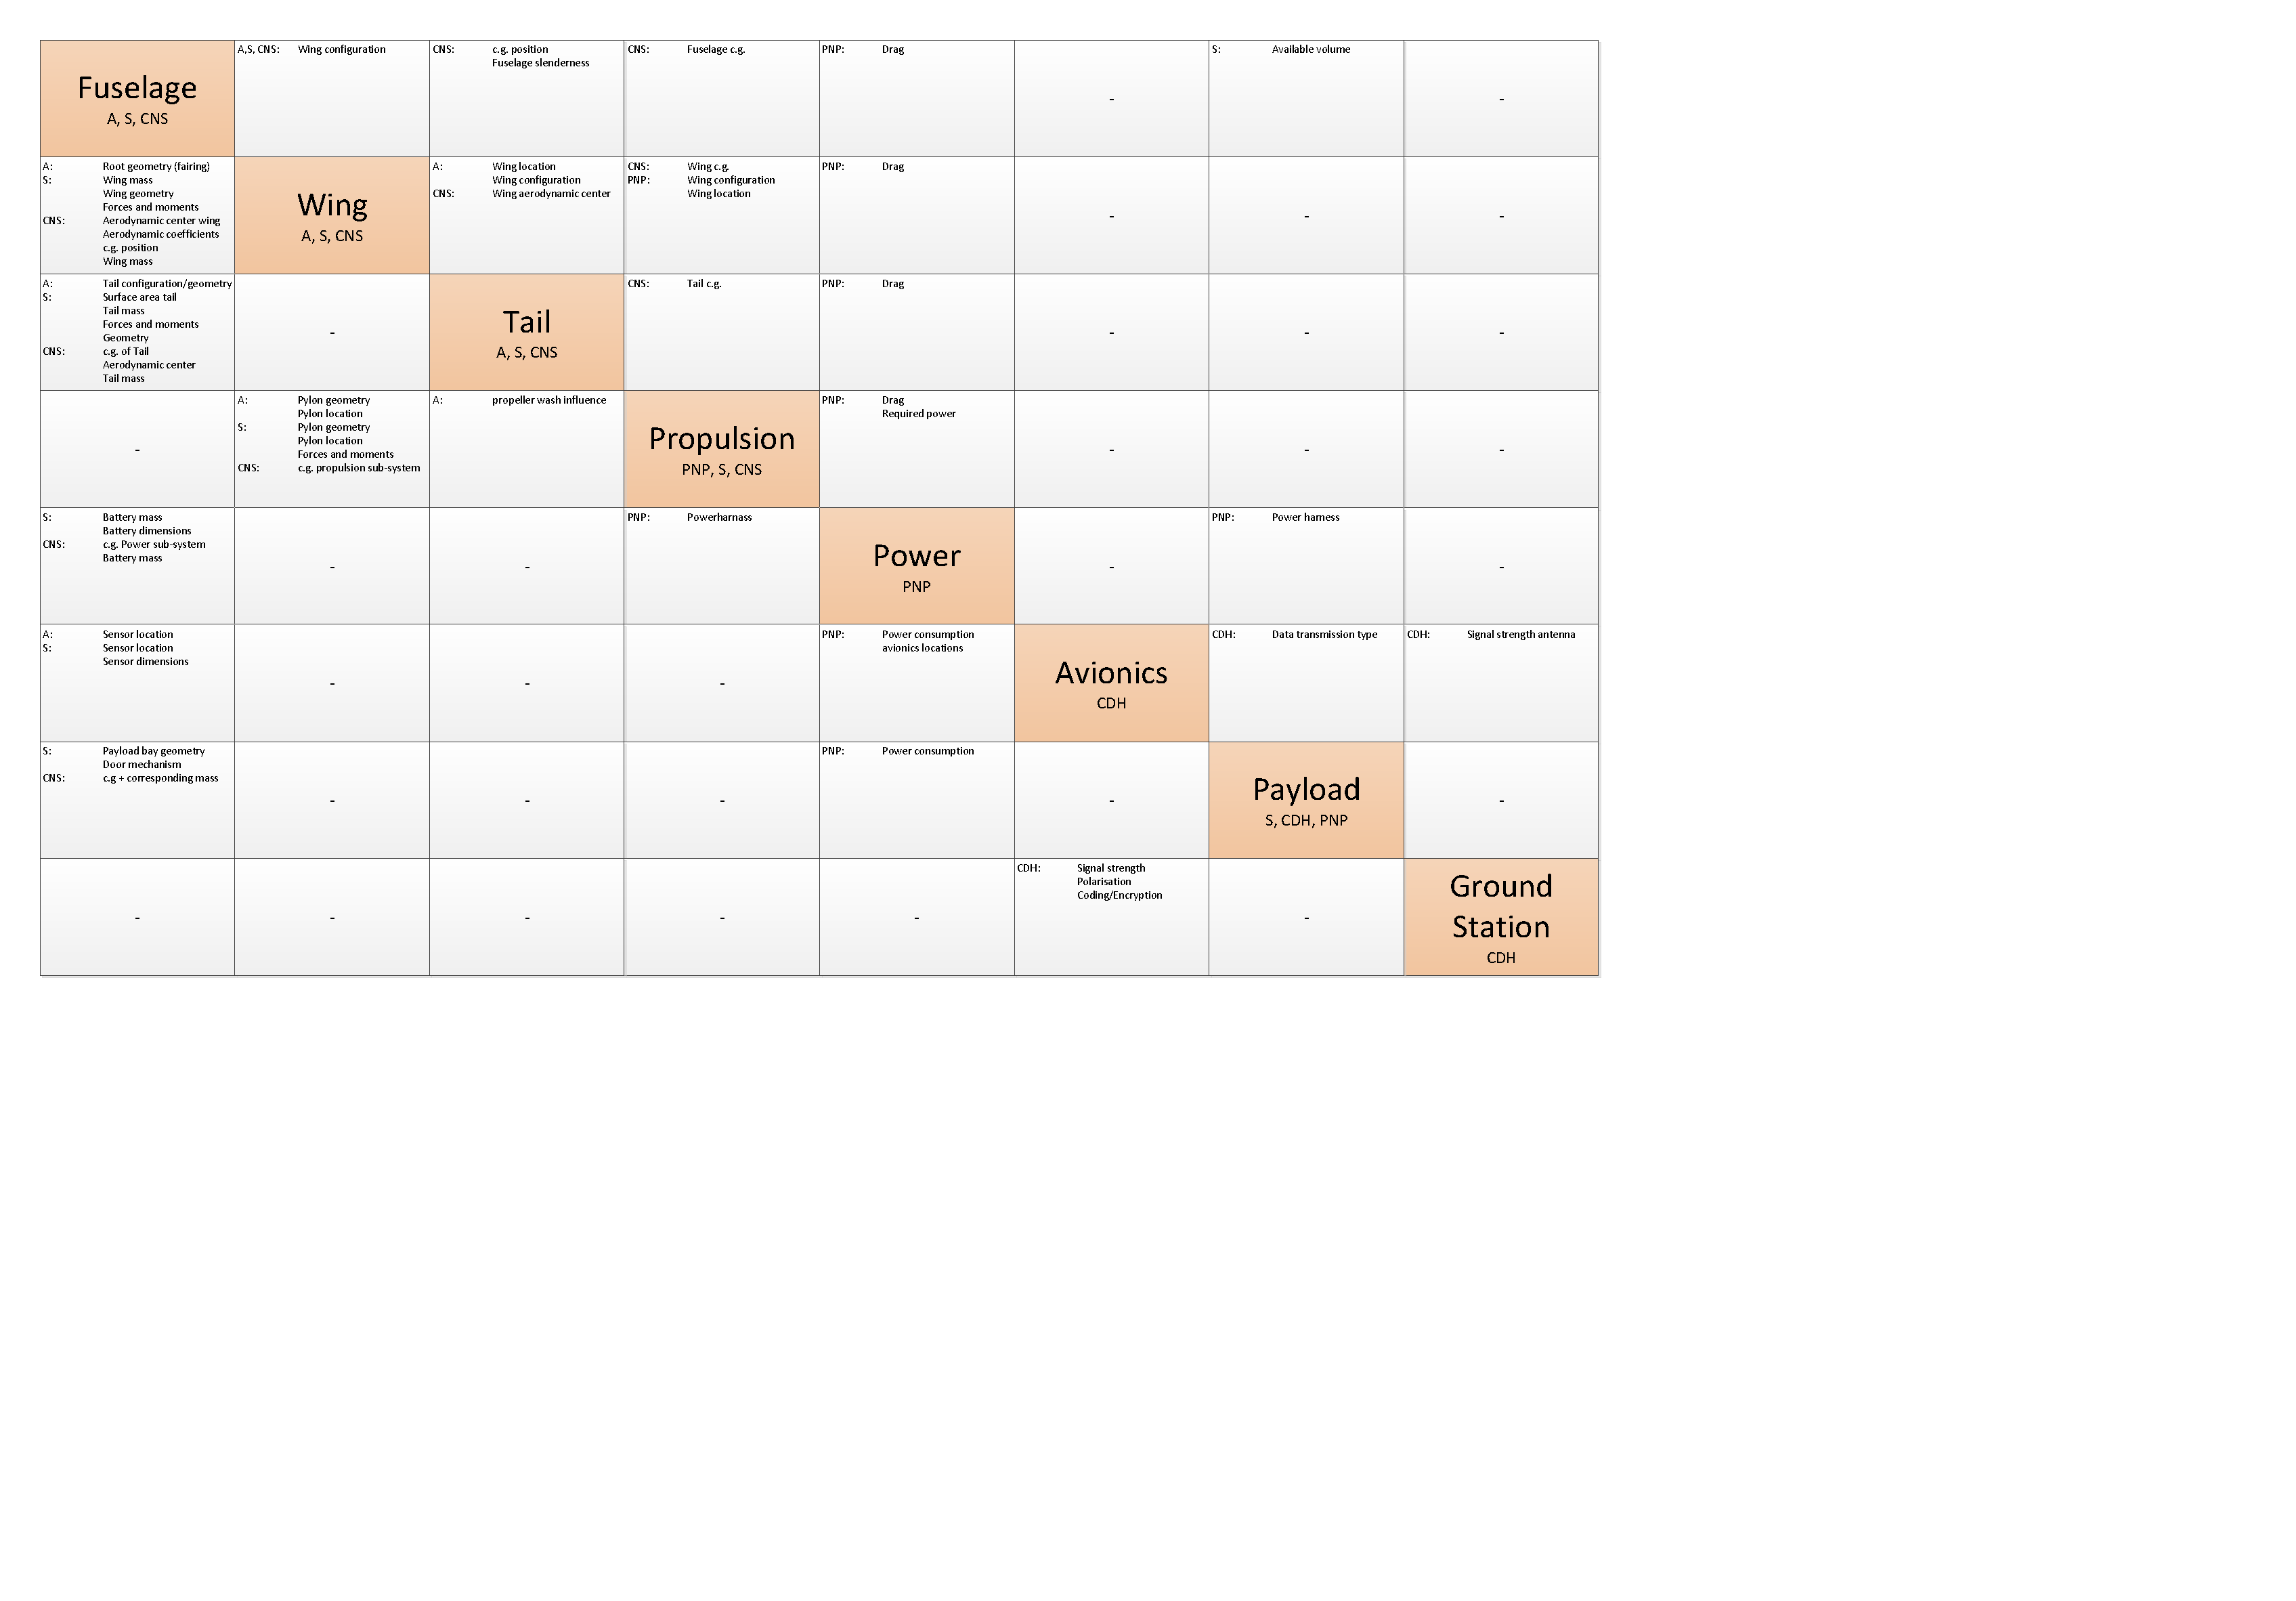
\includepdf[pages=1,fitpaper, scale=0.85,pagecommand={}]{SystemDescription/Figures/N2.pdf}
\label{N2}

\section{Subsystem Requirements}
\label{sec:subs_requ}

The subsystem requirements are presented in this section and are ranked per subsystem. The legend can be found in \autoref{tab:lege}.

\begin{table}[h]
\centering
\caption{Requirements Coding Legend}
\label{tab:lege}
\begin{tabular}{ll}
\toprule
\textbf{Requirement Code} & \textbf{Related to}                       \\\midrule
SUB                       & \textbf{Sub}system                                         \\\hdashline
AV                         & \textbf{Av}ionics                                         \\\hdashline
PR                         & \textbf{Pr}opulsion                                      \\\hdashline
PW                         & \textbf{P}o\textbf{w}er                                 \\\hdashline
W                         & \textbf{W}ing                          \\\hdashline
T                       & \textbf{T}ail       \\\hdashline
F                        & \textbf{F}uselage                      \\\hdashline
P                        & \textbf{P}ayload                      \\\hdashline
GS                        & \textbf{G}round \textbf{S}tation                          \\\bottomrule
\end{tabular}
\end{table}

\subsubsection{Avionics Requirements}
\begin{enumerate}[leftmargin =3.5cm, align=parleft, labelwidth=8em]
    \item[\textbf{SUB-AV-1.1:}] The avionics subsystem shall be able to process flight control and communication data.
    \item[\textbf{SUB-AV-1.2:}] The avionics subsystem shall be insulated to withstand temperatures of -30 to 40 degrees.
    \item[\textbf{SUB-AV-2.1:}] The avionics subsystem shall have a database of restricted areas where it cannot fly.
    \item[\textbf{SUB-AV-2.2:}] The avionics subsystem shall be able to update the restricted areas database.
    \item[\textbf{SUB-AV-2.3:}] The avionics subsystem shall be able to give its geographical position at an accuracy of at least 5 m.
    \item[\textbf{SUB-AV-2.4:}] The avionics subsystem shall be able to determine its distance to the nearest restricted areas.
    \item[\textbf{SUB-AV-2.5:}] The avionics subsystem shall be able to determine its attitude at an accuracy of at least 0.5 degrees per axis.
    %\item[\textbf{SUB-AV-2.6:}] The UAV shall be able to detect weather conditions within [tbd] m.
    \item[\textbf{SUB-AV-2.7:}] The avionics subsystem shall be able to get updates on weather forecasts.
    \item[\textbf{SUB-AV-2.8:}] The avionics subsystem shall be able to return to the base autonomously in case of loss of data link for a period of 10 sec.
    \item[\textbf{SUB-AV-2.10:}] The avionics subsystem shall be able to determine its angular velocity at an accuracy of at least 0.05 deg/sec per axis.
    \item[\textbf{SUB-AV-2.11:}] The avionics subsystem shall be able to determine its angular acceleration at an accuracy of at least 0.01 deg/sec per axis.
    \item[\textbf{SUB-AV-3.1:}] The avionics subsystem shall be able to avoid obstacles.
    \item[\textbf{SUB-AV-3.2:}] The avionics subsystem shall be able to detect all objects within 3 km in front of it.
    \item[\textbf{SUB-AV-3.3:}] The avionics subsystem shall be able to detect the ground when it is within 80 m.
    \item[\textbf{SUB-AV-4.1:}] The avionics subsystem shall be able to fly autonomously.
    \item[\textbf{SUB-AV-4.2:}] The avionics subsystem shall be able to autonomously detect a suitable landing spot.
    \item[\textbf{SUB-AV-4.3:}] The avionics subsystem shall be able to take-off autonomously.
    \item[\textbf{SUB-AV-4.4:}] The avionics subsystem shall be able to land autonomously.
    \item[\textbf{SUB-AV-5.2:}] The avionics subsystem shall automatically descend to 130 m when reaching a height of 150 m.
    \item[\textbf{SUB-AV-6.1:}] The avionics subsystem shall provide a connection to the payload module.
    \item[\textbf{SUB-AV-7.1:}] The avionics subsystem shall make use of a fly-by-wire system.
    \item[\textbf{SUB-AV-8.2:}] The avionics subsystem shall be able to receive inputs from the ground station within a distance of 200 km from the ground station.
    \item[\textbf{SUB-AV-8.3:}] The avionics subsystem shall be albe to transmit data to the ground station within a distance of 200 km from the ground station.
    \item[\textbf{SUB-AV-8.4:}] The data send by the UAV shall be send securely.
    \item[\textbf{SUB-AV-9.1:}] The avionics subsystem shall provide throttle control for motors.
    \item[\textbf{SUB-AV-9.2:}] The avionics subsystem shall control orientation of motors.
\end{enumerate}

\subsubsection{Propulsion Requirements}

\begin{enumerate}[leftmargin =3.5cm, align=parleft, labelwidth=8em]
    %\item[\textbf{SUB-PR-1.1}] The propulsion subsystem shall have a maximum mass of 3.8 kg.
    %\item[\textbf{SUB-PR-1.2}] The propulsion subsystem shall have a maximum cost of 1800 \euro.
    %\item[\textbf{SUB-PR-1.3}] The propulsion subsystem shall require a maximum of 2553 kJ of energy during one mission.
    \item[\textbf{SUB-PR-2.2:}] The propulsion subsystem shall provide thrust in vertical and horizontal flight.
    %\item[\textbf{SUB-PR-2.3:}] The propulsion subsystem shall provide a minimum of 1380 W of power.
    \item[\textbf{SUB-PR-2.4:}] The propulsion subsystem shall provide a minimum thrust of 392 N.
    \item[\textbf{SUB-PR-2.5:}] The propulsion subsystem shall be capable of sustaining a flight velocity of 200 km/h.
    \item[\textbf{SUB-PR-3.4:}] The propulsion subsystem shall be able to provide an angular acceleration of 0.8 $rad/s^{2}$ in roll.
    \item[\textbf{SUB-PR-3.5:}] The propulsion subsystem shall be able to provide an angular pitching acceleration of 0.8 $rad/s^{2}$. 
    \item[\textbf{SUB-PR-3.6:}] The propulsion subsystem shall be able to provide an angular acceleration of 0.1 $rad/s^{2}$ in yaw.
    \item[\textbf{SUB-PR-5.1:}] The propulsion subsystem shall have a maximum noise emission of 68 dB.
\end{enumerate}

\subsubsection{Power Requirements}

\begin{enumerate}[leftmargin =3.5cm, align=parleft, labelwidth=8em]
    \item[\textbf{SUB-PW-1.2:}] The power subsystem shall have a nominal capacity of minimum 1 kWh. 
    \item[\textbf{SUB-PW-1.3:}] The power subsystem shall provide a voltage of 37 V.
    \item[\textbf{SUB-PW-1.4:}] The battery shall be detachable.
\end{enumerate}

\subsubsection{Wing Requirements}

\begin{enumerate}[leftmargin =3.5cm, align=parleft, labelwidth=8em]
    %\item[\textbf{SUB-W-1.1}] The wing subsystem shall have a maximum mass of 4 kg.
    %\item[\textbf{SUB-W-1.2}] The wing shall have a maximum production cost of 900 \euro.
    \item[\textbf{SUB-W-2.1:}] The wing shall provide a minimum lift of 245.25 N in horizontal flight.
    \item[\textbf{SUB-W-2.2:}] The wing shall have a maximum stall velocity of 20 m/s.
    \item[\textbf{SUB-W-2.3:}] The wing tip shall not stall first.
    \item[\textbf{SUB-W-2.4:}] The wing shall have a maximum span of 4.8 meters.
    \item[\textbf{SUB-W-2.5:}] The wing shall have a maximum cantilever ratio of 25.
    \item[\textbf{SUB-W-3.1:}] The wing shall provide sufficient space for its internal components.
    \item[\textbf{SUB-W-3.2:}] The wing shall provide mounting points for the engine pylons. 
    \item[\textbf{SUB-W-3.4:}] The wing shall protect its internal components from dust particles.
    \item[\textbf{SUB-W-3.5:}] The wing shall protect its internal components from precipitation.
    \item[\textbf{SUB-W-3.9:}] The wing shall have a maximum wing tip deflection of 15\% of the wing span.
    \item[\textbf{SUB-W-3.10:}] The wing shall have a maximum wing tip twist angle of $2^{\circ}$.    
    \item[\textbf{SUB-W-3.11:}] The wing shall be designed for a load safety factor of 1.5.
    \item[\textbf{SUB-W-3.14:}] It shall be possible to detach the wing from the fuselage by one person within 2 minutes.
    \item[\textbf{SUB-W-3.16:}] The wing shall not experience aeroelastic flutter at velocities below 220 km/h.
    \item[\textbf{SUB-W-5.6:}] The engine pylons shall not experience aeroelastic flutter at velocities below 220 km/h.
    \item[\textbf{SUB-W-7.2:}] The wing airfoil shall start stalling at the leading edge.
    \item[\textbf{SUB-W-7.3:}] The wing subsystem shall provide an minimal angular roll acceleration of 45 $deg/s^{2}$.   
\end{enumerate}

\subsubsection{Tail Requirements}

\begin{enumerate}[leftmargin =3.5cm, align=parleft, labelwidth=8em]
    \item[\textbf{SUB-T-1.1:}] The tail shall not experience deep stall conditions. 
    \item[\textbf{SUB-T-1.2:}] The tail shall stall after the wing.
    \item[\textbf{SUB-T-2.1:}] The tail shall provide a longitudinal balancing moment for all flight velocities. 
    \item[\textbf{SUB-T-2.2:}] The tail shall be able to provide an angular pitch acceleration of 45 $deg/s^{2}$ in horizontal flight.
    \item[\textbf{SUB-T-2.3:}] The tail shall be able to provide an angular yaw acceleration of 6 $deg/s^{2}$ in horizontal flight.
    \item[\textbf{SUB-T-3.1:}] The tail shall provide sufficient internal space for relevant components.
    \item[\textbf{SUB-T-3.2:}] The tail shall protect internal components from wind.
    \item[\textbf{SUB-T-3.3:}] The tail shall protect internal components from dust. 
    \item[\textbf{SUB-T-3.4:}] The tail shall protect internal components from precipitation.
    \item[\textbf{SUB-T-3.5:}] The tail shall protect internal components from UV radiation.
    \item[\textbf{SUB-T-4.1:}] The tail elevator shall have a maximum deflection angle of 28$^\circ$.
    \item[\textbf{SUB-T-4.2:}] The tail rudder shall have a maximum deflection angle of 25$^\circ$.
    \item[\textbf{SUB-T-5.1:}] The tail shall not contain materials posing a health or environmental threat.
\end{enumerate}

\subsubsection{Fuselage Requirements}

\begin{enumerate}[leftmargin =3.5cm, align=parleft, labelwidth=8em]
    \item[\textbf{SUB-F-1.1:}] The fuselage shall contain at least 1 kg of permanent batteries. 
    \item[\textbf{SUB-F-1.2:}] The fuselage shall provide mounting points for internal and external UAV components.
    \item[\textbf{SUB-F-2.1:}] The fuselage shall protect internal components from wind.
    \item[\textbf{SUB-F-2.2:}] The fuselage shall protect internal components from dust.
    \item[\textbf{SUB-F-2.3:}] The fuselage shall protect internal components from precipitation.
    \item[\textbf{SUB-F-2.4:}] The fuselage shall protect internal component from UV radiation.
    \item[\textbf{SUB-F-3.1:}] The fuselage shall not fail when a belly landing of 4 m/s is performed.
    \item[\textbf{SUB-F-4.1:}] The fuselage shall not contain materials that pose health or environmental threats.
\end{enumerate}

\subsubsection{Payload Requirements}

\begin{enumerate}[leftmargin =3.5cm, align=parleft, labelwidth=8em]
    \item[\textbf{SUB-P-2.1:}] The payload subsystem shall have a two-way power link with the fuselage.
    \item[\textbf{SUB-P-2.2:}] The payload subsystem power link shall be rated for a minimum of 50 W.
    \item[\textbf{SUB-P-3.3:}] The payload subsystem shall provide mounting points for the payload (including additional batteries).
    \item[\textbf{SUB-P-3.4:}] The payload subsystem shall allow for payload release during flight.
\end{enumerate}

\subsubsection{Ground Station Requirements}

\begin{enumerate}[leftmargin =3.5cm, align=parleft, labelwidth=8em]
    \item[\textbf{SUB-GS-2.1:}] The ground station shall be able to process all data received by the UAV. 
    \item[\textbf{SUB-GS-3.2:}] The ground station battery shall enable at least two hours of consequal operating.
    \item[\textbf{SUB-GS-4.1:}] The ground station shall transmit inputs to the UAV within a distance of 200 km.
    \item[\textbf{SUB-GS-4.2:}] The ground station shall be able to receive data from the UAV within a distance of 200 km.
    \item[\textbf{SUB-GS-4.3:}] The ground station shall send data towards the UAV securely.
    \item[\textbf{SUB-GS-4.7:}] The ground station shall be able to communicate with the drone in stormy weather conditions.
    \item[\textbf{SUB-GS-5.1:}] The ground station casing shall fit within 100x50x30 cm.
    \item[\textbf{SUB-GS-5.2:}] The ground station shall weigh at most 7.5 kg.
    \item[\textbf{SUB-GS-5.3:}] All ground system components shall be easily replaceable.
    \item[\textbf{SUB-GS-6.2:}] The ground station shall have a display that can show mission specific information.
    \item[\textbf{SUB-GS-6.3:}] The ground station shall be able to control the UAV.
    \item[\textbf{SUB-GS-6.4:}] The ground station shall be able to make the UAV drop the payload.
    \item[\textbf{SUB-GS-7.1:}] The ground station shall displaye a warning when exceeding a height of 140 m from the ground.
    \item[\textbf{SUB-GS-7.2:}] The ground station shall display a warning when approaching a restricted area.
\end{enumerate}




\section{Budgets \& Contingencies}
\label{sec:budg_cont}
To ensure that the departments do not exceed any limits during the designing, some budgets have been made. On top of the budgets a contingency is added. There are two budgets: the mass budget and the cost budget. The ground control is not considered in the budgets as it is seen as a separate system. The final budgets and contingencies for mass and cost can be found in \autoref{tab:massbudget}. 

\begin{table}[H]
    \centering
    \caption{Mass and Cost Budget for the Aircraft}
    \label{tab:massbudget}
    \begin{tabular}{ccccc} \toprule
    
    
    
    \bfseries Subsystem     & \bfseries Mass Budget &\bfseries Contingency & \bfseries Cost Budget &\bfseries  Contingency \\ \midrule
    Power     & 8.0 kg & 5\% & 800 EUR& 5\%  \\
    Propulsion & 4.0 kg & 5\% & 2200 EUR& 10\% \\
    Avionics & 1.0 kg & 5\% & 2200 EUR & 10\% \\
    Wing & 3.5 kg & 10\% & 800 EUR& 10\% \\
    Tail & 1.5 kg & 10\% & 400 EUR& 10\% \\
    Fuselage & 2.5 kg & 10\% & 800 EUR& 10\% \\
    Payload & 4.5 kg & 5\% & 300 EUR& 5\% \\ \bottomrule
    \end{tabular}
\end{table}


\paragraph{Mass Budget}
The mass budget has been estimated by comparing it to a similar UAV, the Avy One\footnote{\url{avy.eu}, Accessed on 21-06-2017}. This aircraft has a Manufacturing Empty Weight (MEW) of 13 kg, meaning that if this design has a maximum mass of 25 kg, 12 kg are allotted to the battery and payload. The other 13 kg are destined for the structure of the aircraft\footnote{Private Contact Avy, 22-05-2017}. The mass budget can be seen in \autoref{tab:massbudget}. To have an allowable margin of freedom, contingencies are put in place for each subsystem. The percentage of the contingency varies with the certainty of the mass budget. The contingency should decrease over time as the project progresses, and the mass prediction becomes more precision.

\paragraph{Cost Budget}
Analysing the cost budget has been done in a similar fashion as the mass budget. Contact has been established between Atmos, a company which produces the Marlyn\footnote{\url{http://www.atmosuav.com/}, Accessed on 22-06-2017}, a UAV similar to the Winged Quadcopter. This company provided information about how much percent of the cost their subsystems take up. Before budgeting the cost of each subsystem, the choice has been made to separate the cost of materials from the cost of manufacturing. The assumption has been made that 75\% of the costs are attributed to manufacturing. This leaves 7.5k EUR for materials of the subsystems. The percentage of cost for the Marlyn can be seen in \autoref{tab:costperc}\footnote{Private Contact Atmos, 08-06-2017}.

\begin{table}[H]
    \centering
    \caption{Percentage of Cost for the Atmos UAV}
    \begin{tabular}{rl} \toprule
    \bfseries Subsystem &\bfseries Percentage of Cost \\\midrule
    Power \& Propulsion     &  20\% \\
    Payload     & 10\% \\
    Avionics & 20\% \\
    Wing, Tail \& Fuselage & 40\% \\
    Contingency & 10\% \\\bottomrule
    \end{tabular}

    \label{tab:costperc}
\end{table}

With these values, it is possible to devise the cost budget. The Atmos UAV has its cameras added to the payload cost, which this design does not have. This means that a part of their payload cost can be neglected. Atmos has said that the avionics will take up a larger percentage of the total cost for this design since they have designed and built parts of the avionics by themselves. The wing and fuselage turn out to cost the same amount, while the tail costs half of the wing \cite{costbreakdown}. 

Using the preliminary energy calculation from the midterm report \cite{midterm}, the cost of the power subsystem is estimated to be 800 EUR. The rest of the cost is attributed to the propulsion subsystem, which turns out to be close to 20\% as estimated by Atmos. The final cost budget can be seen in \autoref{tab:massbudget}.


    \chapter{Power \& Propulsion}
\setlength{\parindent}{15pt}
\label{ch:powe_prop}

\section{Design Approach}
\label{sec:DAPNP}
% include WFD

\autoref{fig:wfdpnp} shows the Work Flow Diagram of the design process executed by the Power \& Propulsion department. It included both the design of the motor with propellers, as the power source with power distribution system. 

The design process starts with the propulsion unit designed, after that the power unit is designed. This approach is chosen since it is more convenient to first select the right motors and afterwards come up with a corresponding battery unit. The first design block, indicated with a blue shade in \autoref{fig:wfdpnp}, covers the design approach of the propulsion unit: the motor with propellers. 

\subsection*{Propulsion Unit Design Approach}
The first step in that design block is the defining of the propulsion configuration; this means determining the number of motors and their mounting location. An analysis was done for a number of motors ranging from three to five. Also different locations were analysed, such as wing and body mounted. After the determination of the number of motors with their corresponding location, the kind of motor was chosen. Requirement SYS-VS-3 states that the UAV shall have electrical propulsion. Although propulsion type was constrained, motor type still had to be decided on; a choice had to be made between brushed and brushless motors. This was done by comparing the advantages and disadvantages of both motor types in a qualitative way.

%%Explain what needs to be why analysed! 
For the propulsion unit performance, the following analysis approach was applied.

1) high-velocity requirement SYS-PF-1.2 is a driving requirement. This means we first need to ensure this performance characteristics. The most important design aspect to attain this 200km/h is the propeller design; a high pitch is required. 

\begin{comment}
For analysis

show a pitch of 14 inch is needed. The approximated flight speed of this propeller with the max. RPM is:

\begin{equation*}
    14*0.0254* \frac{9302}{60} = 55.13 m/s
\end{equation*}

A propeller with this propeller in combination with this RPM will enable the UAV flight the required 200km/h.

\end{comment}















































\paragraph{Thrust Calculations VTOL:} For the right motor choice, a python tool was developed that gives the maximum thrust output in VTOL as function of the maximum power output ($P_{max}$) and area of the propeller ($A_{prop}$). The right motor was found in an iterative way; different motor specifications were used as input to see if the required output was met. For the development of this tool, the conservation of momentum in helicopter climb/hover theory was used\footnote{\url{http://s6.aeromech.usyd.edu.au/aerodynamics/index.php/sample-page/aircraft-performance/hoverclimbdescent-analysis/}, Accessed 19-06-2017}. The equation for required thrust for hovering and climb are shown in \autoref{eq:hc}

\begin{equation}
\label{eq:hc}
    T_{total,req} = (2 \rho A P_{req}^{2})^{\frac{1}{3}}
\end{equation}

The required thrust value was provided by the Control \& Stability. This maximum value was computed with the extreme values for the c.g. position. For instance, with the most aft c.g. position, the aft motors have to provide a significant higher thrust levels. Furthermore, also a margin had to be taken into account for the case a motor has to stabilise an incoming gust; during hovering the thrust setting should not exceed 75\% for instance to still have margin to correct disturbances.\\

\paragraph{Thrust \& Power Calculations for Horizontal Flight Phase:} For the horizontal flight phase, only the aft motors are operative, they deliver thrust while the propellers on the front motor are folded (feathering mode). 

First the required power in horizontal flight was evaluated by means of a python tool. This was done by computing the drag at maximum airspeed and multiplying this by the flight velocity. The following equation for required power for high-velocity cruise flight was derived\footnote{\url{http://nptel.ac.in/courses/101104007/Module2/Lec6.pdf}, Accessed 09-06-2017}. This was obtained by replacing $C_{L}$ by the weight divided by the dynamic pressure (q) and surface (S):
\begin{equation*}
    P_{req} = D V = C_{D} q S V = (C_{D_{0}} + \frac{C_{L}^{2}}{\pi AR e}) q S V
\end{equation*}

\begin{equation}
    P_{req} = \frac{1}{2} \rho V^{3} S C_{D_{0}} + \frac{\frac{W^{2}}{\frac{1}{2} \rho V S}}{\pi AR e}
\end{equation}


If all four motors would contribute, the chosen configuration would create propeller wash phenomena since the motors are aligned in longitudinal direction. This might influence the performance of the aft propeller. Furthermore, there is also a strongly relation to propeller performance: \\

4) Required Thrust and power horizontal flight
5) Propeller design

The performance of the propellers is very sensitive for the operational regime; away from the design point, the propeller performs poorly. Propellers are designed for specific conditions. 

In the design of this UAV, the propellers have to provide propulsion both in VTOL mode and in high-velocity cruise flight

VTOL: which is low velocity with high required thrust

High-velocity horizontal flight: which means lower required thrust but high velocity. This will result in a significantly high required RPM and propeller pitch, with a low desired propeller area

%%---------DONE TO HERE------%%


This means, the aft motors are optimised for horizontal flight, since their function is to sustain the UAV in horizontal phase.

How to do hybrid operations with the same props????? Solutions:

- By optimising the front ones for VTOL and make them the main VTOL contributors, the aft motors are optimised for horizontal operations. In this way they can assist partly in the VTOL phase and serve as main contributor to the horizontal flight phase. 
COOLTOOL!!! 


\subsection{Power Subsystem Design Approach*}



\section{Assumptions}
\label{sec:AssuPNP}

\begin{itemize}
    \item Assumption 1
\end{itemize}

\section{Analysis} %% MUST BE REVISED !!!!!
\label{sec:AnalPNP}
This analysis contains the design steps taken in the process of designing a propulsion and power system that meets the prior set requirements. This also explains the subdivision of this section into a motor and propeller part (propulsion) and an energy source subsection (Power).

\subsection{Motor and Propellers}

\paragraph{Motor configuration:} Different amount of motors with corresponding locations were analysed. The different locations are leading edge mounted, wing mounted quadcopter setting and body mounted. The amount of motors varied from three to five. The analysed configurations can bee seen in \autoref{fig:motorconfig}.

% Include figure with mounting positions and diff. amount of motors.

\begin{itemize}
    \item \textbf{Three motors:} After consulting the Control \& Stability department, three motors was not considered an option since it does not create sufficient controllability in VTOL operations.
    \item \textbf{Four motors:} After calculations, an amount of four motors turned out to be sufficient to meet both the required thrust and power output in VTOL and in high-velocity cruise. After consulting with Control \& Stability, wing quadcopter setting was chosen over body mounted configuration; the greater moment arm increases the effectiveness of the motors in VTOL stability. 
    \item \textbf{Five motors:} This was regarded as an solution to the later discussed problems with the propeller design. However, a fifth relatively heavy horizontal flight sustainer would cause conflicts with both the cost and mass budget. 
\end{itemize}

\paragraph{Motor Types} There are two kind of motors; brushed or brushless. Brushed motors have the disadvantage of a relative lower efficiency. However, the cost for these motors is considerably lower. Brushless on the other hand, have a higher cost, but their efficiency is higher. The cost increase can be covered by the budget, the increased efficiency is regarded dominant over the cost increase. Therefore there is chosen for a brushed motor. Upon recommendation of ATMOS, there was chosen to use the catalogue of Hacker-motors\footnote{\url{https://www.hacker-motor-shop.com/}, Accessed 19-06-2017}.\\
%% ELABORATE AND CONNECT TO THE TABLE!!!!! AND EXPLAIN OUTCOME!!!
\begin{table}[H]
    \centering
    \caption{Brushed vs. Brushless analysis}
    \label{tab:bbanal}
    \begin{tabular}{m{3cm}>{\centering}m{2cm}>{\centering}m{2cm}m{7cm}}
        \toprule        \textbf{}                                      & \centering\textbf{Brushed} & \centering\textbf{Brushless} & \textbf{Note}                                                                                                                                                                                                                           \\ \midrule
        \textbf{Efficiency}                            &                  & \cmark             & Brushed ranges from 75\% - 80\% in contrast to brushless, which ranges from 85\% - 90\%.\footnote{\url{https://quantumdevices.wordpress.com/2010/08/27/brushless-motors-vs-brush-motors-whats-the-difference/}, Accessed 20-06-2017} \\ \hdashline
        \textbf{Cost}                                  & \cmark           &                    & Brushed motors are typically lower in cost due to the simplicity and established production techniques\cite{wp}.                                                                                                                      \\\hdashline
        \textbf{Velocity Range}            &                  & \cmark             & Brushless motors typically generate higher RPM and torque meaning it can operate with the higher pitched propeller. The combination of a high pitch and RPM enable higher velocity range for the brushless motor\cite{dae}.                       \\\hdashline
        \textbf{Reliability}                           &                  & \cmark             & Brushless motors have less part can potentially break of wear-out\footnote{\url{http://www.nmbtc.com/brushless-dc-motors/why-brushless-motors/}, Accessed 20-06-2017}.                                                               \\\hdashline
        \textbf{Environmental Resistance} & \cmark           &                    & Due to the brushed motors simpilicity, they can deal with environments that are more hostile towards electronics and motor components\cite{dae}.                                                                                                  \\\hdashline
        \textbf{Noise Emission}                      &                  & \cmark             & Brushless motors create less noise emissions due to completely enclosure of internal components\footnote{\url{http://www.nmbtc.com/brushless-dc-motors/why-brushless-motors/}, Accessed 20-06-2017}.                                  \\ \bottomrule
    \end{tabular}
\end{table}
If all four motors would contribute, the chosen configuration would create propeller wash phenomena since the motors are aligned in longitudinal direction. This might influence the performance of the aft propeller. Furthermore, there is also a strongly relation to propeller performance: \\

\paragraph{Propeller performance:}
The performance of the propellers is very sensitive for the operational regime; away from the design point, the propeller performs poorly. Propellers are designed for specific conditions. 

In the design of this UAV, the propellers have to provide propulsion both in VTOL mode and in high-velocity cruise flight

VTOL: which is low velocity with high required thrust

High-velocity horizontal flight: which means lower required thrust but high velocity. This will result in a significantly high required RPM and propeller pitch, with a low desired propeller area

%%---------DONE TO HERE------%%


This means, the aft motors are optimised for horizontal flight, since their function is to sustain the UAV in horizontal phase.

How to do hybrid operations with the same props????? Solutions:

- By optimising the front ones for VTOL and make them the main VTOL contributors, the aft motors are optimised for horizontal operations. In this way they can assist partly in the VTOL phase and serve as main contributor to the horizontal flight phase. 
COOLTOOL!!! 



\subsection{Energy Source}

3) Power:
- Battery that sustain the motors (VTOL, high-speed) and all the other subsystem (Look into the C-rating, discharge value.);
- Cable harness (layout, mass estimation, regard accessibility and Assembly capabilities);
- Electrical component and circuits design.

\section{Verification \& Validation}
\label{sec:VNVPNP}

\section{Results}
\label{sec:RPNP}

- 4 motors; 2 types of motors with corresponding propellers.

All four are used for the VTOL phase. only  the aft motors are used as pushers for the horizontal cruise phase

- two front: Q60-2M, Aeronaut CAM Carbon 16x10
- two aft: A50-12L, APC 11x14


%fix the centering issue

\begin{table}[H]
\centering
\caption{Off-the-shelf component choice Power \& propulsion subsystems}
\label{PNPresults}
    \begin{tabular}{m{3cm}m{3.2cm}m{0.6cm}m{2.64cm}m{2.64cm}}
    \toprule
    \textbf{Component}                   & \textbf{Product Name}                                                     & \textbf{Q.} & \textbf{Unit Mass {[g]}} & \textbf{Unit Cost{[\euro]}} \\ \midrule
    \textbf{Front Motor}        & Hacker Q60-7M                                                             & 2           & 520                        & 410                      \\\hdashline
    \textbf{Front Propeller}    & AC Carbon 16x10                                                           & 2           & 25                         & 11.8                      \\\hdashline
    \textbf{Front Speed Controller} & MasterSPIN 99 Pro                                                         & 2           & 105                        & 229                      \\\hdashline
    \textbf{Aft Motor}          & Hacker A50-12L                                                            & 2           & 445                        & 184                      \\\hdashline
    \textbf{Aft Propeller}      & APC 11x14                                                                 & 2           & 40                         & 3.50                       \\\hdashline
    \textbf{Aft Speed Controller}   & X-70-SB                                                                   & 2           & 54                         & 99                       \\\hdashline
    \textbf{DC/DC Converter}    & ...                                                                       & 2           & ...                        & ...                        \\\hdashline
    \textbf{Rotating Mechanism}     & ...                                                                       & 4           & ...                        & ...                        \\\hdashline
    \textbf{Servo}              & ...                                                                       & 4           & ...                        & ...                        \\\hdashline
    \textbf{Battery}            & Zippy Compact 5800mAh 10s Lipo                                            & 6           & 1283                       & 80.55
    \\\hdashline
    \textbf{Cabling}            & Turnigy HQ 8 AWG Silicon wire                                             & -           & 120 /m                     & 3.50 /m                 \\ \bottomrule
    \end{tabular}
\end{table}


\begin{comment}
Recommandations???

4) Optional: look into other propulsion types (break with electric prop. requirement):
- Electric VS. Combustion
- Electric VS. Hybrid propulsion
\end{comment}
    \chapter{Aerodynamic Analysis}
\setlength{\parindent}{15pt}
\label{ch:aero_anal}

The aerodynamic analysis for horizontal flight only will be performed in this chapter, seeming that for vertical flight the airspeed will be low. The aircraft will need to fulfil a set of requirements which concern the aerodynamic properties of the aircraft. The most important aerodynamic property is the lift, since the aircraft will need to generate enough lift to be able to fly. The problem is that with lift comes drag. The challenge will be to design an aircraft which satisfies the requirements, while producing as little drag as possible.

The first section in this chapter is the approach, which is important to ensure that the process of designing goes well. The next section contains the assumptions made to ease the design process. The following section contains the actual analysis made for all the aerodynamic parts of the aircraft. Finally, once the analysis is done, the used methods are verified and validated. 

\section{Design Approach}

There are several aspects of the plane that need an aerodynamic analysis, each of these aspects will be designed to have the least amount of drag as possible. The problem that arises is that the design with the least drag probably will not coincide with the requirements or the constraints put up by other departments. This results in an iterative process which will ensure that the design with the least drag, and that complies with requirements and constraints, comes out best. To get an overview of the design process, \autoref{fig:flow:aerodynamics} shows the process followed in the form of a work flow diagram.

\begin{figure}[hbt]
    \centering
    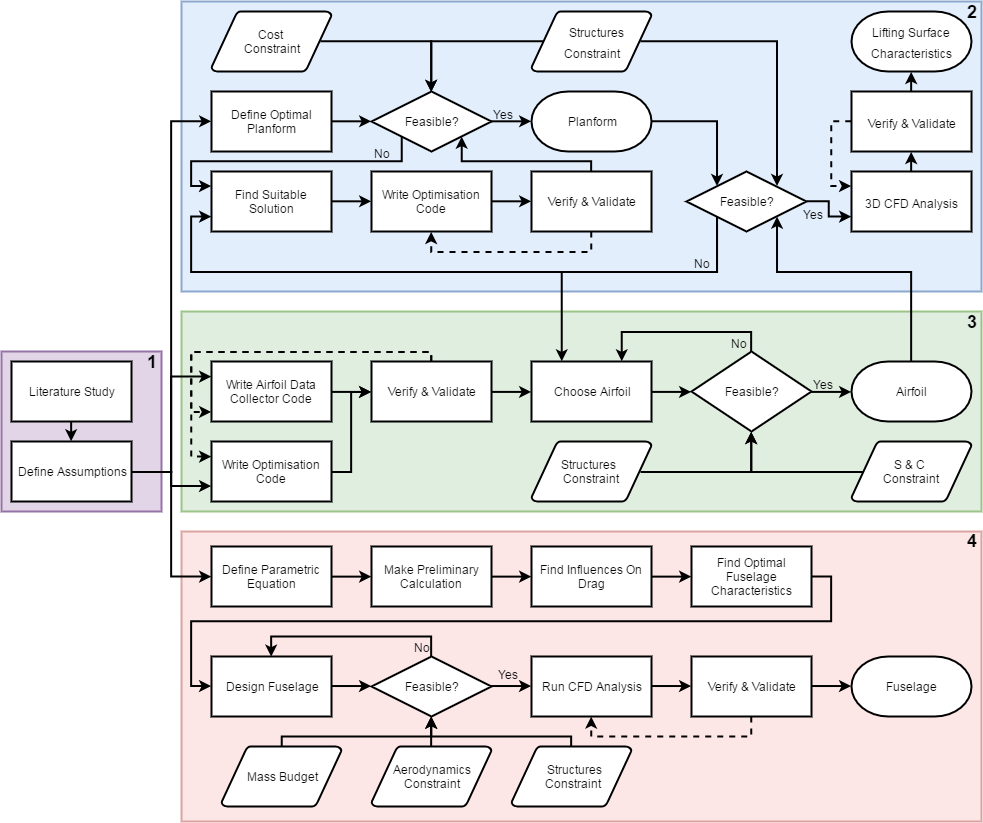
\includegraphics[scale=0.45]{Aerodynamics/Figures/AerodynamicWFD.png}
    \caption{Work Flow Diagram for the Aerodynamic Design Process}
    \label{fig:flow:aerodynamics}
\end{figure}

The work flow diagram shows four differently coloured regions. These are the separate processes that have been carried out, though not only four processes have taken place. The first region is the preparatory work needed to be done before the designing can start. The literature study will help with understanding how to perform the design, and the assumptions will be made to give an overview of how the design can be done. Once that is finished, it is possible to go to any of the other regions based on what needs to be designed.

The second region contains the work flow diagram for the sizing and shaping of both the wing and the tail. The processes for both these subsystems are very similar, hence they have the same work flow diagram. The first step of the process is to define the optimal planform, which would be the one with the least amount of induced drag. Once that is done, it needs to be checked if the planform is feasible with the constraints set by the structures department. If feasible, then the planform is done. If it is not feasible, then an alternate solution has to be determined. With the help of a Python code the optimal alternative can be found, and again checked to be feasible. Now, if it is not feasible, the iteration starts to find the correct planform.

The third region is the work flow diagram for the airfoil selection for both the wing and the tail. Before this process can start, code has to be written to collect all airfoil data and select the optimal airfoil. Verification and validation will check if the code used is correct. Once all the data is collected and the optimisation is made, the airfoil will be checked for feasibility, constrained by the structures department and the stability \& control department. If the airfoil turns out to be infeasible, a new airfoil optimisation will be run with new constraints to find the new best airfoil.

The fourth region is used for the design of the fuselage and the pylon. To start off the process, several parametric equations are selected which are used to make preliminary calculations. Once the calculations are done, it is possible to find the major influences of the fuselage shape on the drag. Knowing these influences, the optimal fuselage characteristics can be found, with which it is possible to design the fuselage. Once again, when the fuselage is designed, it needs to be checked for feasibility. This time the constraints come from the structures department, the aerodynamics department and the mass budget. If the design is feasible, a Computational Fluid Dynamics [CFD] analysis can be done to find more precise aerodynamic characteristics. The results of the CFD analysis are reflected against the parametric equations to check whether the CFD analysis has been implemented correctly.

\nomenclature[A]{CFD}{Computational Fluid Dynamics}

\section{Assumptions}

\begin{itemize}
    \item The flight condition is assumed to be at an altitude of 120 meters. This has been chosen because the majority of missions will not be flown at higher altitudes, so it will be optimised for a 120 meter altitude. When flying at a higher altitude, the aircraft will need to fly at a higher angle of attack to achieve enough lift, increasing the drag and decrease the overall performance.
    \item The increment in velocity due to the pusher propellers is assumed to be negligible, not affecting the wing aerodynamics. In reality the propellers will increase the speed over the wing and decrease the amount of detached airflow, which increases the lift over the wing.
    \item The lifting surfaces are assumed to be completely smooth. In reality there are imperfections and other aspects, e.g. attachments, which decrease lift and increase drag.
    \item The drag of the propellers and motors is neglected. In reality they produce drag, but due to a lack of resources it was not possible to analyse this.
    \item The upwash and downwash of the wing on the pylons is neglected. In reality this effect would create a destabilising positive pitching moment. Nevertheless, ignoring this is acceptable as the pylons are narrow and the resulting pitching moment will be orders of magnitude smaller than the one created by the wing and tail.
    \item It is assumed that for the CFD analysis the boundary layer is completely laminar. In reality, the boundary layer will transition to a turbulent flow, yet it is assumed that the transition point is near the aft of each geometry. The direct effect is a lower skin friction drag than in the case when the transition is not neglected. \cite[75]{anderson}, \cite[170]{fluidmech}.
    \item It is assumed that for the CFD analysis the turbulence model is laminar. Since most geometries of the UAV are smooth, slender, and have a small angle of attack, it is assumed that in reality the transition from a laminar to a turbulent flow would not occur.
\end{itemize}

\section{Analysis}

This section will contain the analysis of the various subsystems. The goal of the analysis is to find the optimal solution to the problems at hand by meeting the requirements given with the set of constraints set by other departments. The first subsystem to be analysed is the wing in \autoref{sec:aero_wing}. Next, the tail will be analysed in \autoref{sec:aero_tail}, and the fuselage is analysed in \autoref{sec:aero_fuse}. The last subsystem analysed is the power \& propulsion subsystem, though only the pylon will be analysed. This analysis can be seen in \autoref{sec:aero_pylo}.

\subsection{Wing}
\label{sec:aero_wing}

There are five things that need to be analysed for the wing. The first aspect to be analysed is the shape \& size of the wing, which gives the wing planform. Afterwards, the airfoil can be found which will give the wing the best aerodynamic properties. When that is done, a look will be taken into the high lift devices to see if they are necessary. Finally, with the basic wing shape designed, it is possible to analyse the wing in a 3D environment, to see if the aerodynamic characteristics are still satisfied. Finally, the winglets are the last aspect of the wing to be checked.

\subsection*{Shape \& Size}

\paragraph{Literature Study} For low speed aircraft, there is one major influence of the wing on the drag, namely the induced drag\footnote{\url{https://www.grc.nasa.gov/www/k-12/airplane/induced.html}, Accessed on 14-06-2017}. Seeming this UAV flies at low speeds (20-55 $\frac{m}{s}$), the induced drag will be the biggest source of drag of the wing. To minimise the drag, the lift distribution of the wing needs to be elliptical, which can be achieved by having an elliptical planform. This would be the optimum planform of the wing, as can be seen in \autoref{fig:flow:aerodynamics}. However, an elliptical wing is harder to manufacture due to its complex shape \cite{ellipticalmanu}. Due to this, an alternative has to be found, which still resembles an elliptical lift the best. This can be done by using several taper ratios or having a different airfoil at different spanwise locations. Due to the seeming complex manufacturing of different spanwise airfoils, the choice has been made to have several different tapers to resemble an elliptical lift distribution.

Another aspect of the planform which has been looked at is the sweep of the wing. Usually the front is swept to reduce mach bubbles being created on the wing, which reduces lift drastically and generates a lot of drag. But this effect occurs only at high speeds (M \textgreater 0.8) so it is not necessary for this UAV to have it. Having a swept wing will only have an adverse effect by reducing the chord wise speed over the wing, hence reducing lift. If the lift decreases, a bigger surface area will be needed which would only increase the drag.

Having a wing stall can have an adverse effect on the safety of the aircraft, it gets even worse if the tip stalls before the root. This is because this will create a moment on the aircraft, which will roll the aircraft uncontrollably. This rolling can cause the aircraft to plummet to the ground, especially when close to the ground during landing. To prevent the tip stalling before the root, the tips will have washout. This causes the wing tips to have a lower incidence angle with respect to the rest of the wing, making it have a lower angle of attack. Due to the lower angle of attack, the tips will stall later and hence prevent tip stalling.

\paragraph{Method} The sizing of the wing has been done by looking at the wing loading. The surface area needed to generate enough lift depends on various factors, see \autoref{eq:liftgenerate}.

\begin{equation}\label{eq:liftgenerate}
    S = \frac{2\cdot W}{C_{L}\cdot V^2\cdot \rho}
\end{equation}

Using air density at sea level and the stall speed of 20 $\frac{m}{s}$, it is possible to find the wing loading for different $C_{L}$ values. The best $C_{L}$, at a feasible wing loading, is 1.3. With this number the surface area of the planform is calculated to be 0.8 $m^2$.

Since the optimum solution (an elliptical planform) is not feasible, it is necessary to find the best alternative solution. With the choice to have several different taper ratios, it has been chosen to use two different taper ratios on the wing. This choice has been made because the wing has to be detachable for ground handling, so the location of the taper change will be where the wing is detachable. Having more than two tapers would implicate the manufacturing while improving the planform slightly. 

To find the best planform, a python code has been made. The code has been made in such a way that it would iterate through all variables directly or indirectly to find all possible combinations of planforms. The variables can be seen in \autoref{tab:dimensionswing}. Each planform generated has been compared to an elliptical planform, using the mean squared error of the differences of normalised chord lengths. This way the planform which resembles an ellipse the most could be chosen. To verify the planform for its elliptical lift, the program XFLR5 has been used, which can generate the lift of a 3D wing and show its distribution. The resulting lift distribution can be seen in \autoref{fig:wdist} in \autoref{sec:aero_vali}.

\paragraph{Results}

With the design process done, the planform of the wing is finalised. The result can be seen in \autoref{fig:wingplanform}. The dimensions of the planform are summarised in \autoref{tab:dimensionswing}.

\begin{figure}[H]
    \centering
    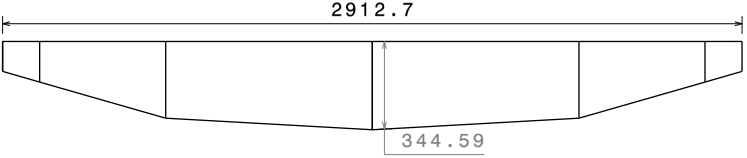
\includegraphics[scale=0.75]{Aerodynamics/Figures/wingplanform}
    \caption{Planform of the Wing, Dimensions in mm}
    \label{fig:wingplanform}
\end{figure}

\begin{table}[H]
    \centering
    \caption{Dimensions of the Wing}
    \label{tab:dimensionswing}
    \begin{tabular}{llll}\toprule
\bfseries    Variable     &\bfseries  Value &\bfseries Variable &\bfseries Value\\ \midrule
    $c_{t_w}$     & 118mm & $c_{r_w}$ & 348mm\\
    $b_w$ & 2920mm & $AR_w$ & 10. \\
    $\lambda_{tip}$ & 0.39 & $\lambda_{root}$ & 0.8 \\
    $l_{twist}$ & 146mm & $l_{taperchange}$ & 642mm \\
    Twist angle at tip & $5^{\circ}$ & &\\ \bottomrule
    \end{tabular}
\end{table}



\nomenclature[B]{$c_{t_{w}}$}{Tip chord of wing \nomunit{m}}
\nomenclature[B]{$c_{r_{w}}$}{Root chord of wing \nomunit{m}}
\nomenclature[B]{$b_w$}{Span of wing \nomunit{m}}
\nomenclature[B]{$AR_w$}{Aspect Ratio of wing \nomunit{-}}
\nomenclature[G]{$\lambda_{tip}$}{Taper ratio at tip of wing\nomunit{-}}
\nomenclature[G]{$\lambda_{root}$}{Taper ratio at root of wing\nomunit{-}}
\nomenclature[B]{$l_{twist}$}{Length of twist on wing (one side) \nomunit{m}}
\nomenclature[B]{$l_{taperchange}$}{Length where taper changes, as seen from the tip \nomunit{m}}
\nomenclature[B]{$C_L$}{Lift coefficient \nomunit{-}}

\subsection*{Airfoil}

\paragraph{Literature Study} It is possible to achieve lift by employing various methods, one being the use of airfoils. These produce lift while minimising their drag contribution. Therefore it possible to achieve high efficiency, which in turn depends on the airfoil geometry. Airfoils are classified into families, and depending on which family the airfoil belongs to, different parameters are used to describe the geometry. Airfoils within one family will show similar shape characteristics, which also distinguish them from the other families. Since the aerodynamic performance is directly influenced by the shape, every airfoil family will therefore have distinct aerodynamic characteristics. Thus the application of the airfoil serves as the starting point for airfoil selection, starting with the selection of the airfoil family.

The most common airfoil families are the NACA 4-, 5-, and 6-digit series. The geometries of these airfoils are defined by the maximum camber value and position, the maximum thickness, and the family-specific parametric equations. Since the Hybrid UAV must be able to transition from horizontal to vertical flight, it is essential that the airfoil is predictable at low velocities and high angles of attack ensuring a safe transition. Therefore, the airfoil chosen for the Hybrid UAV must demonstrate gentle stall behaviour, which is true only with the NACA 4-digit series \cite{naca_series}. For this series, the first digit indicates the maximum camber, the second specifies the position of the maximum camber, and the last two digits indicate the maximum thickness of the airfoil. All these values are shown as a percentage of the chord.

Apart from the general aerodynamic behaviour, the airfoil's lift and drag (or $C_{l}$ and $C_{d}$) relationship must also be considered since it dictates the efficiency. In the case of the Hybrid UAV, two ratios are of greatest importance, namely $\frac{C_{l}}{C_{d}}$ influences the maximum range, and $\frac{C_{l}^{1.5}}{C_{d}}$ influences the maximum endurance \cite{perf}. Since the Hybrid UAV will mostly fly in cruise condition, the aim is to maximise both of these ratios for the lift coefficient required at cruise velocity, effectively yielding the optimal airfoil.

\paragraph{Method} The selection of the airfoil was done in two steps. Firstly, a list of all possible NACA 4-digit series airfoils was generated, with parameters ranging from 0008 to 5530. These were then inspected for their maximum lift coefficient and all airfoils which had a $C_{l,max}$ lower than 1.3 (dictated by the stall velocity) were discarded. 

The second step consisted of calculating the $\frac{C_{l}}{C_{d}}$ and $\frac{C_{l}^{1.5}}{C_{d}}$ at a $C_{l}$ value of 0.56 ($C_{l,cruise}$) for the remaining airfoils. Next, the airfoil with the highest $\frac{C_{l}}{C_{d}}$ ratio, and the airfoil with the highest $\frac{C_{l}^{1.5}}{C_{d}}$ ratio was found, yielding two airfoils optimised either for maximum range, or maximum endurance.

\paragraph{Results} The result of the airfoil selection yielded only one airfoil, namely the NACA 4417. This means that this airfoil has the highest $\frac{C_{l}}{C_{d}}$ and $\frac{C_{l}^{1.5}}{C_{d}}$ at $C_{l,cruise}$, and therefore is optimal for both maximum range and endurance. Its geometry can be seen in \autoref{fig:4417geo}.

\begin{figure}[H]
    \centering
    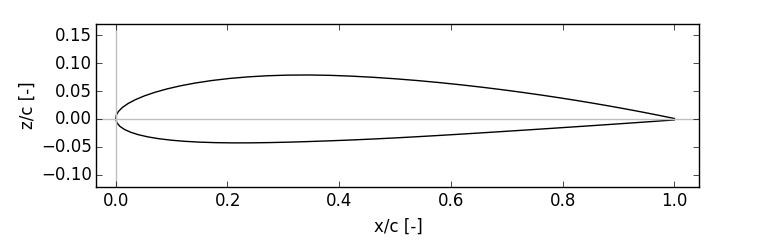
\includegraphics[scale=0.75]{Aerodynamics/Figures/4417geo}
    \caption{NACA 4417 Airfoil Geometry}
    \label{fig:4417geo}
\end{figure}
The aerodynamic characteristics of this airfoil are summarised in \autoref{tab:naca4417}. It should be noted that according to this analysis, the wing incidence angle is $1^{\circ}$ ensuring the highest efficiency in cruise flight.

\nomenclature[B]{$C_l$}{Lift coefficient of airfoil \nomunit{-}}
\nomenclature[B]{$C_{l,cruise}$}{Lift coefficient of airfoil during cruise \nomunit{-}}
\nomenclature[B]{$C_d$}{Drag coefficient of airfoil \nomunit{-}}


\begin{table}[H]
\centering
\caption{NACA 4417 Lift and Drag Characteristics}
\label{tab:naca4417}
\begin{tabular}{lcc}
\toprule
      & \textbf{Value} & \textbf{$\alpha$ {[}deg{]}} \\ \midrule
\textbf{$C_{l,max}$}    & 1.53  & 14                        \\ \hdashline
\textbf{$(C_{l}/C_{d})_{Cl,cruise}$} & 57.6  & 1                         \\ \hdashline
\textbf{$(C_{l}^{1.5}/C_{d})_{Cl,cruise}$} & 41.4  & 1                         \\ \bottomrule                                                                                
\end{tabular}
\end{table}

\subsection*{High Lift Devices}

\paragraph{Literature Study} High lift devices are necessary in aircraft to be able to fly at lower stall speeds, because the high lift devices increase the $C_{L}$ of the wing. This proves to be useful for large aircraft, so that the landing speed can be reduced significantly, ensuring a safer landing. However, the Hybrid UAV does not need to land horizontally, meaning that this is not a problem. High lift devices can still be implemented to be able to ensure a lower stall speed, but adding high lift devices brings forward more disadvantages than advantages. They will increase the overall cost of the aircraft due to extra material cost and manufacturing costs and it brings complexity in the wing which is unnecessary. More loads will be introduced, hence more structural integrity will be needed. These factors alone are the reason why the choice has been made not to use high lift devices.

\subsection*{3D Wing}

\paragraph{Literature Study} Determining the total lift and drag of the wing is essential when assessing the feasibility of the design. To do so, a three-dimensional analysis has to be performed which would mainly take into account the effect of the wingtip vortexes caused by the finite span. Two tools capable of such an analysis were found.

The first tool is XFLR5. It is an airfoil analysis tool also suitable for basic 3D wing analyses. For this software it was found that the horseshoe Vortex Lattice Method (VLM) is most fitting for the analysis since it allows non-flat wings to be analysed (the current wing has wing tip washout resulting in an out-of-plane geometry) \cite[26]{xflr}. In addition, XFLR5 has the option to include the effects of viscosity in the horseshoe VLM.

\nomenclature[A]{VLM}{Vortex Lattice Method}

The second tool is the SimScale Workbench, a CFD software. Starting with the meshing, it was found that the hex-dominant parametric meshing algorithm (included with the software) was most efficient and lead to faster convergence times \cite[9]{ansys}. Next, due to the very low Mach numbers, the fluid dynamics were selected to be incompressible. Furthermore, the turbulence model was selected to be laminar as explained previously in the assumption section. Finally it was found that smooth solvers are more efficient and therefore they were used as well \cite{iter}.

 It is expected that, with the use of the 3D analysis tools, the total lift will be smaller than $\frac{1}{2}\rho V^{2} S C_{l}$, the stall behaviour will be more gradual \cite[72]{ruijgrok}, and the total drag will be higher than $\frac{1}{2}\rho V^{2} S C_{d}$, where $C_{l}$ and $C_{d}$ are the airfoil lift coefficients.

\paragraph{Method} The 3D analysis was first carried out in XFLR5. The wing geometry was created within the tool and the surface was divided into panels. The panel distribution along the span is uniform (constant panel width), but along the chord a cosine distribution is used (panel size decreases towards the leading and trailing edge). Next, the viscous horseshoe vortex lattice method was chosen as the analysis definition. The analysis was ran with an initial velocity of 30 m/s and an angle of attack of $1^{\circ}$. The results were exported and analysed to find the total lift, drag, pitching moment, and lift distribution. Due to the iterative nature of the wing design, this process was repeated whenever necessary, and the results were updated. During the design iterations only XFLR5 was used for the 3D analysis since it could produce updated results within minutes, ensuring a smoother design process.

Once the wing design was fixed, the SimScale Workbench was used to determine the lift and drag with higher accuracy. First the wing geometry was imported into the program, and the corresponding surface and bounding-box meshes were created. The bounding box was made sufficiently large such that the boundary effects could be neglected. In addition, a second smaller mesh box was defined around the wing which consisted of a finer mesh. Next the inlet, outlet, and wall boundary conditions were set for the bounding box and wing surface. Finally, the simulation was started with an initial inlet velocity of 30 m/s. The analysis yielded the lift as well as the pressure and viscous drag.

\paragraph{Results} The first results of the XFLR5 analysis are seen in \autoref{tab:xflrwing}. As predicted, the total lift is lower than the one required to achieve flight at cruise conditions. Therefore an iteration was performed by increasing the $C_{l,cruise}$ and checking whether the previous airfoil remained the most efficient one. Since this was indeed the case, the wing incidence angle was changed to $2.5^{\circ}$, according to the 2D airfoil angle of attack corresponding to the new cruise lift coefficient. The results of the updated incidence angle are also seen in \autoref{tab:xflrwing}. The lift-drag polar for the wing can be seen in \autoref{fig:polar}.

\begin{table}[H]
\centering
\caption{Main Wing XFLR5 Results}
\label{tab:xflrwing}
\begin{tabular}{lccc}
\toprule
&\bfseries First Results &\bfseries Iterated Results & \\ \midrule
\textbf{$C_{L,cr}$}   & 0.444 & 0.622 & {[}-{]} \\\hdashline
\textbf{$L_{cr}$}    & 195.8 & 274.3 & {[}N{]} \\\hdashline
\textbf{$C_{D,cr}$}   & 0.015 & 0.02 & {[}-{]} \\\hdashline
\textbf{$D_{cr}$}    & 6.615 & 8.82 & {[}N{]} \\\hdashline
\textbf{$C_{M,ac}$} & -0.137  & -0.137  & {[}-{]} \\ \bottomrule
\end{tabular}
\end{table}

\begin{figure}[H]
    \centering
    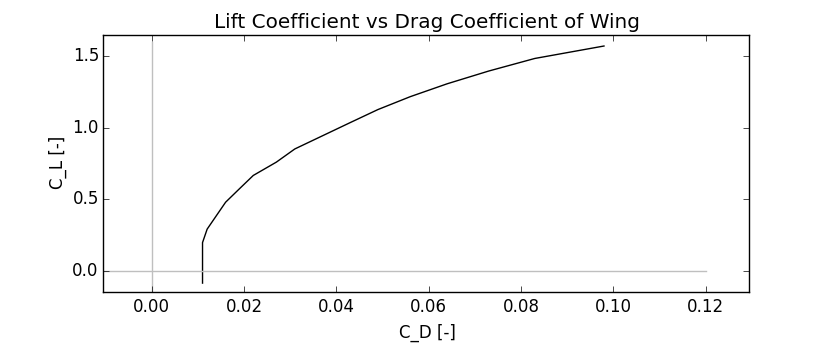
\includegraphics[width=0.8\textwidth]{Aerodynamics/Figures/wpol}
    \caption{Lift-drag Polar for the Wing}
    \label{fig:polar}
\end{figure}

The results of the SimScale Workbench CFD analysis with the updated wing incidence angle yielded a total lift of 173 N and a total drag of 6 N at cruise velocities. The validity of this result is discussed in \autoref{sub:vval}.

\subsection*{Wingtip Devices}

\paragraph{Literature Study} Wingtip devices such as winglets decrease the drag of a wing by reducing the magnitude of the tip vortices. This means the efficiency of the plane increases when using wingtips, although the factor it increases by is too low for further consideration\footnote{Prive Meeting with Mark Voskuijl, 15-06-2017}. Having the improved efficiency from the winglets does not overcome the disadvantages it brings with it. Having winglets increases the overall cost due to extra material for the surface and the internal structures (higher wing loading). Seeming the efficiency gained is not worth it, it has been decided not to use winglets.

\subsection{Tail}
\label{sec:aero_tail}

Only three aspects have to be analysed for the tail. The three aspects are similar to the wing, the shape, the airfoil and the 3D tail. The size of the tail will not be designed by the aerodynamics department because the surface area of the tail is of more value for the stability \& control department. The aspect to be analysed is the shape, which is done to design the planform of the tail (with the given surface area of the stability \& control department). The second aspect is the airfoil of the tail, which needs to comply with constraints set by the stability \& control department. The final aspect is the 3D tail, which is an aspect to be analysed because the 3D characteristics will differ compared to the 2D characteristics.

\subsection*{Shape}

\paragraph{Literature Study} There are two parts of the tail which need to be shaped and sized, namely the horizontal and the vertical tail. The empennage will be a T-tail type, chosen by the stability and control department. This means that the vertical tail will be closed in by the horizontal tail and the fuselage. Due to this, the vertical tail has been shaped in such a way that it would just fit between these two other parts of the aircraft. The horizontal tail however, has been shaped to minimise the drag. Just as for the wing, the minimal drag occurs when there is an elliptical lift distribution. This time, it is possible to achieve this with an elliptical planform due to three reasons. The first reason being that the loads on the horizontal tailplane are low, meaning the inner structure can be small and less complex. Furthermore, the size of the tailplane is much smaller than that of the wing, easing the manufacturing. The last reason is that the tailplane is not as complex as the wing. Due to these reasons the horizontal tailplane has been chosen to have an elliptical planform.

\paragraph{Method} The key to getting a elliptical lift distribution is to have the chord lengths follow the size of an ellipse, although the centre of the ellipse can be moved around. Keeping in mind that the elevators are most efficient if perpendicular to the flow, the horizontal centre line of the planform has been moved down to the three-quarters chord point. This way the elliptical lift distribution is kept while having a more effective controllability with the elevators. 

Having an elliptical lift distribution is not indicative of the root chord and span of the tailplane, so to size these dimensions reference aircraft have been used. The usual aspect ratio of a horizontal tailplane is between four and five\footnote{\url{http://nptel.ac.in/courses/101106035/035_Chapter\%206_L26_(04-10-2013).pdf}, Accessed on 20-6-2017}, for the vertical tail a taper ratio between 0.3-0.6 is common \cite{verticaltailtaper}. With these values, and the surface areas acquired from the stability \& control department, the final dimensions could be calculated for both the vertical and horizontal tailplane.


\paragraph{Results} With the shaping done, it is possible to find the dimensions of the tail surfaces. The dimensions of the tailplanes can be seen in \autoref{tab:taildimen}, the planforms of the horizontal tailplane and the vertical tailplane can be seen in \autoref{fig:htail} and \autoref{fig:vtail}, respectively.

\begin{table}[H]
    \centering
    \caption{Tail Dimensions}
    \label{tab:taildimen}
    \begin{tabular}{cc:cc}\toprule
    \multicolumn{2}{c}{\bfseries Horizontal Tail} & \multicolumn{2}{c}{\bfseries Vertical Tail} \\\midrule
    Parameter     &  Value & Parameter & Value\\ \midrule
    $c_{r_h}$     & 196mm & $c_{r_v}$ & 181mm\\ \hdashline
    $b_h$ & 694mm & $b_v$ & 220mm\\ \hdashline
    $AR_h$ & 4.5 & $AR_v$ & 3.35\\ \hdashline
    $\lambda_h$ & - & $\lambda_v$ & 0.45 \\\bottomrule
    \end{tabular}
\end{table}

\begin{figure}[H]
    \centering
    \begin{minipage}{0.45\textwidth}
        \centering
        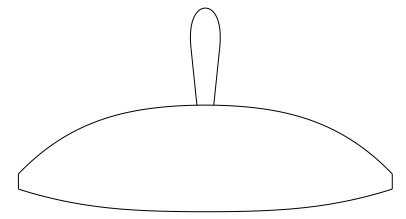
\includegraphics[width=0.9\textwidth]{Aerodynamics/Figures/htail} % first figure itself
        \caption{Top View of the Horizontal Tailplane, On Top Of The Vertical Tailplane}
        \label{fig:vtail}
    \end{minipage}\hfill
    \begin{minipage}{0.45\textwidth}
        \centering
        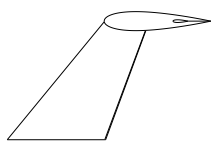
\includegraphics[width=0.9\textwidth]{Aerodynamics/Figures/vtail} % second figure itself
        \caption{Side View of the Vertical Tailplane}
        \label{fig:htail}
    \end{minipage}
\end{figure}

\nomenclature[B]{$c_{r_h}$}{Root chord of horizontal tail \nomunit{m}}
\nomenclature[B]{$c_{r_v}$}{Root chord of vertical tail \nomunit{m}}
\nomenclature[B]{$b_h$}{Span of horizontal tail \nomunit{m}}
\nomenclature[B]{$b_v$}{Span of vertical tail \nomunit{m}}
\nomenclature[B]{$AR_h$}{Aspect ratio of horizontal tail \nomunit{-}}
\nomenclature[B]{$AR_v$}{Aspect ratio of vertical tail \nomunit{-}}
\nomenclature[G]{$\lambda_v$}{Taper ratio of vertical tail \nomunit{-}}
\nomenclature[G]{$\lambda_h$}{Taper ratio of horizontal tail \nomunit{-}}






\subsection*{Airfoil}

\paragraph{Literature Study} The horizontal tail must stall later than the main wing to ensure stability, therefore the corresponding airfoil must have a larger stall angle than the one chosen for the main wing. Although the function of the horizontal plane is different from the main wing, the 4-digit NACA series is chosen here again as the starting point. This, again, is due to the predictable stall characteristics. In addition, this family is also common amongst tail airfoils \cite[23]{airtail}. Nevertheless, the main difference between the wing and the tail is that the tail usually uses a symmetrical airfoil since it must provide positive and negative lift. 

The required $C_{l_{h}}$ at cruise conditions (dictated by the stability \& control department) must also be kept in mind when selecting the airfoil, such that the tail will produce as little drag as possible during cruise, while keeping the UAV stable. Apart from the airfoil itself, the tail cruise lift coefficient can be changed by the horizontal plane incidence angle, yet the aim is to minimise this angle too.

\nomenclature[B]{$C_{l_{h}}$}{Airfoil lift coefficient of horizontal tail \nomunit{-}}

The vertical tail must produce the least amount of drag, therefore an appropriate airfoil must be chosen. The 4-digit NACA series is chosen for the vertical tail as well since, again, it is commonly used on tails. The only constraint on the vertical tail airfoil is the minimum thickness (dictated by the structures department), which in turn also depends on the vertical plane planform.

\paragraph{Method} The optimal horizontal tail airfoil was found by inspecting symmetrical NACA airfoils ranging from 0008 to 0029 for both the $C_{l_{h}}$ required at cruise conditions and the stall angle. It was decided that the stall angle should be about $4^{\circ}$ greater than the stall angle of the main wing. Out of all possibilities, the airfoil with the lowest thickness was chosen.

The optimal vertical tail airfoil was found by calculating the thickness of the vertical tailplane and comparing it to the structures department's requirement. The airfoil with the lowest sufficient thickness was chosen.

\paragraph{Results} The horizontal tailplane airfoil with the lowest thickness that satisfied the lift and stall requirements was the NACA 0018. The aerodynamic characteristics are summarised in \autoref{tab:naca0018}.

\begin{table}[H]
\centering
\caption{NACA 0018 Aerodynamic Characteristics}
\label{tab:naca0018}
\begin{tabular}{lcc}
\toprule
\textbf{$C_{l,cruise}$}  & 0.18 & [-] \\ \hdashline
\textbf{$C_{l,max}$}     & 1.24 & [-] \\ \hdashline
\textbf{$C_{d,cruise}$}  & 0.009 & [-] \\ \hdashline
\textbf{$\alpha_{stall}$} & 17.1 & [deg] \\ \bottomrule
\end{tabular}
\end{table}

The vertical tailplane airfoil with the lowest thickness that satisfied the Structures department's requirement was the NACA 0012. The zero lift drag coefficient ($C_{d_{0,v}}$) is 0.007.

\nomenclature[B]{$C_{l,max}$}{Airfoil maximum lift coefficient \nomunit{-}}
\nomenclature[B]{$C_{d,cruise}$}{Airfoil drag coefficient at cruise \nomunit{-}}
\nomenclature[G]{$\alpha_{stall}$}{Airfoil stall angle \nomunit{deg}}
\nomenclature[B]{$C_{d_{0,v}}$}{Airfoil zero-lift drag coefficient of vertical tail \nomunit{-}}

\subsection*{3D Tail}

\paragraph{Literature Study} The knowledge gained from the 3D Wing literature study is directly applicable to the 3D tail analysis. Again, it is expected that the 3D total lift will be smaller than the estimated 2D lift, and the 3D drag will be larger than the estimated 2D drag.

\paragraph{Method} The horizontal and vertical tailplane 3D analyses were first carried out in XFLR5 in the same manner as the main wing. The only difference is the angle of attack, which was now set to $0^{\circ}$ for both the horizontal and vertical plane. Hence, the horizontal plane has a incidence angle of $0^{\circ}$ as dictated by the stability \& control department.

Once the tail design was fixed, the SimScale Workbench was used again to determine the lift and drag with higher accuracy. This analysis was also carried out in the same manner as the main wing.

\paragraph{Results} The results of the XFLR5 tail analysis are seen in \autoref{tab:xflrhtail}. As predicted, the 3D lift coefficient of the horizontal tailplane is lower than the one required at cruise conditions. Therefore an iteration was performed by increasing the incidence angle of the horizontal plane to $2.6^{\circ}$. The iterated results are also shown in \autoref{tab:xflrhtail}.

\begin{table}[H]
\centering
\caption{XFLR5 Tail Results}
\label{tab:xflrhtail}
\begin{tabular}{lcccc}
\toprule
 & \textbf{Horizontal} & \textbf{Iterated Horizontal} & \textbf{Vertical} & \\ \midrule
\textbf{$C_{L,h}$}   & 0.118 & 0.181 & 0 & {[}-{]} \\ \hdashline
\textbf{$L_{h,cr}$}    & 6.96 & 10.68 & 0 & {[}N{]} \\ \hdashline
\textbf{$C_{D,h}$}   & 0.0015 & 0.0016 & 0.0003 & {[}-{]} \\ \hdashline
\textbf{$D_{h,cr}$}    & 0.65 & 0.71 & 0.128 & {[}N{]} \\ \bottomrule
\end{tabular}
\end{table} 

\nomenclature[B]{$C_{L,h}$}{Horizontal tail lift coefficient \nomunit{-}}
\nomenclature[B]{$L_{h,cr}$}{Horizontal tail lift at cruise \nomunit{N}}
\nomenclature[B]{$C_{D,h}$}{Horizontal tail drag coefficient \nomunit{-}}
\nomenclature[B]{$D_{h,cr}$}{Horizontal tail drag at cruise \nomunit{N}}

The results of the SimScale Workbench indicate a lift of 12.57 N and a drag of 1.11 N for the combined vertical and horizontal planes. The validity of these results is discussed in \autoref{sub:vval}.

\subsection{Fuselage}
\label{sec:aero_fuse}

\paragraph{Literature Study} From the point of view of the aerodynamics, the fuselage shape must be designed such that it produces the least amount of drag as possible during cruise flight. Based on the Roskam parametric equations for the fuselage drag, the two independent variables directly influencing the drag are the maximal frontal area and the length of the fuselage \cite[44]{roskam}.

Parametric equations serve as a starting point for the optimisation of the fuselage shape and provide an estimate on the drag, yet to gain more accurate results 3D analysis must be performed. Unfortunately XFLR5 does not support body analysis, therefore only the SimScale Workbench CFD tool is used for this purpose. Here, the knowledge gained from the 3D Wing literature study is directly applicable to the 3D fuselage analysis as well.

\paragraph{Method} First, the subsonic parametric equations for the drag of the fuselage were coded in python. These equations took into account the wing-fuselage interference, the skin friction contribution, the lift induced drag, and the influence of the general shape of the fuselage on the drag. Next, since the maximum frontal area and the length of the fuselage are independent variables, the drag of the fuselage was calculated for a range of both of these two inputs and plotted. This plot indicated how these two inputs influenced the drag, and made it possible to optimise the fuselage shape for minimal drag.

Once the fuselage shape was fixed, the CFD analysis was performed in order to gain more accurate drag values. This analysis was also carried out in the same manner as the main wing.

\paragraph{Results} The influence of the maximum frontal area and the fuselage length on the drag is shown in the plot in \autoref{fig:fusdrag}. It can be seen that for fuselage lengths smaller than 3 meters, a smaller frontal area results in a smaller drag coefficient. Furthermore, for each frontal area there is an optimal fuselage length resulting in a minimal drag coefficient. 

\begin{figure}[H]
    \centering
    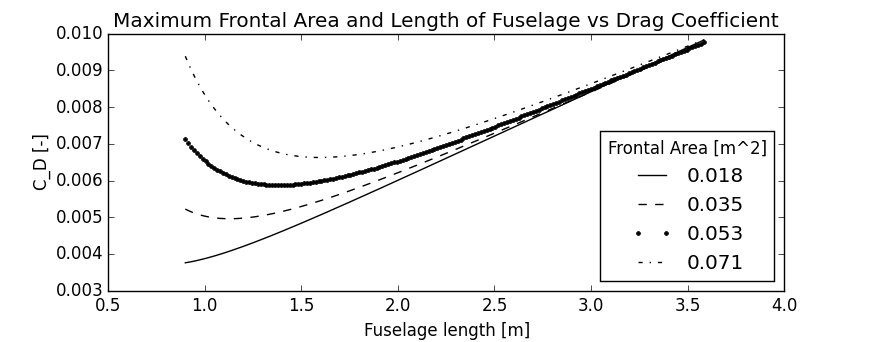
\includegraphics[width=0.8\textwidth]{Aerodynamics/Figures/fusdrag}
    \caption{Influence of Maximum Frontal Area and Fuselage Length on Drag Coefficient}
    \label{fig:fusdrag}
\end{figure}

Since the cross sectional area of the fuselage is mostly dictated by the payload bay and the structures department, the maximum frontal area is fixed at $0.053 m^{2}$. At this frontal area, the optimal fuselage length is 1.4 meters. The minimal length was limited to 1.7 meters by the structures department, nevertheless the final fuselage length was set to 1.8 meters. The reason for this was to have a less abrupt fuselage ending by elongating the empennage by 10 centimetres, in anticipation of a lower pressure drag. Although this contradicts the optimisation, it should be noted that the parametric equations assume that the fuselage cross sectional area gradually decreases towards the aft of the UAV, and this is not the case for the Hybrid UAV. To approximate this situation, the empennage is elongated, resulting in a $C_{D}$ of 0.0062 and a drag of 2.7 N at cruise velocities.

\nomenclature[B]{$C_{D}$}{Drag coefficient \nomunit{-}}

The results of the SimScale Workbench indicate a drag of 2.2 N during cruise. The validity of this result is discussed in \autoref{sub:vval}.

\subsection{Pylon}
\label{sec:aero_pylo}

\paragraph{Literature Study} The design of the pylon is performed in a similar fashion to the fuselage, with the goal to minimise the drag. Therefore the knowledge gained from the fuselage literature study is directly applicable to the pylon design. Furthermore, the same parametric equations can be used as for the fuselage \cite[73]{roskam}. The pylon-fuselage interference is considered significant enough to be included in the analysis, therefore the relevant parametric equations should also be used \cite[77]{roskam}.

\paragraph{Method} The parametric equations for the pylon were coded in the same manner as the one for the fuselage, with the addition of the pylon-fuselage interference equation. In this case, the two independent variables were the pylon length and the pylon diameter, and the output was the drag coefficient of the pylon. The results were plotted which made it possible to optimise the design for minimal drag.

Once the pylon shape was fixed, the CFD analysis was performed in order to gain more accurate drag values. This analysis was also carried out in the same manner as the main wing.

\paragraph{Results} The influence of the pylon diameter and length on the drag is shown in the plot in \autoref{fig:pyldrag}. It can be seen that the smaller the diameter, the smaller the drag coefficient. Furthermore, for each diameter there is an optimal pylon length resulting in a minimal drag coefficient.

\begin{figure}[H]
    \centering
    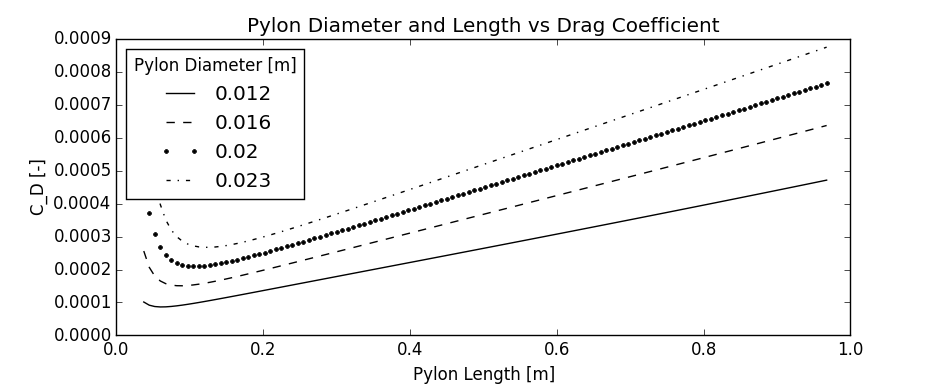
\includegraphics[width=0.8\textwidth]{Aerodynamics/Figures/pyldrag}
    \caption{Influence of Pylon Diameter and Length on Drag Coefficient}
    \label{fig:pyldrag}
\end{figure}

The minimal diameter is dictated by the structures department, therefore it is fixed at 2 cm. The corresponding optimal pylon length is 10.5 cm, yet the minimal possible length set by the stability \& control department is 90 cm. The result of the parametric analysis is a $C_{D}$ of 0.00072 and a drag of 0.317 N at cruise velocities.

The results of the SimScale Workbench indicate a drag of 0.248 N during cruise. The validity of this result is discussed in \autoref{sub:vval}.

\section{Verification \& Validation}
\label{sec:aero_vali}

In order to ensure that the 3D analyses were carried out correctly, the methods have to be verified, and the results validated. The verification of the XFLR5 tool is considered first. The validation of the wing, tail, fuselage, and pylon results is treated afterwards.

\subsection{XFLR5 Verification}

XFLR5 uses an inviscid linear-vorticity panel method to calculate the aerodynamic characteristics of airfoils \cite[1]{xfoil}. Therefore, in order to test whether this model produces accurate results within XFLR5, two verification methods are used. For convenience, the NACA 4417 airfoil will be used as an example.

\paragraph{Analytical} The first method consists of finding the $C_{l}-\alpha$ curve using the classical cambered thin airfoil theory \cite[348]{anderson}, where the lift coefficient is described by \autoref{eq:cl_anal}:

\begin{equation}
\label{eq:cl_anal}
    C_{l} = \pi \Big{(}2\alpha+\frac{2}{\pi}\int_{0}^{\pi}\frac{dz}{dx}\cos{\theta}d\theta-\frac{2}{\pi}\int_{0}^{\pi}\frac{dz}{dx}d\theta\Big{)}
\end{equation}
Here, $z$ describes the mean camber line geometry as a function of the chord position $\frac{x}{c}$. For the 4-digit NACA family, the derivative of the mean camber line geometry with respect to the chord position is given by \autoref{eq:naca_geo1} and \ref{eq:naca_geo2}\footnote{\url{http://airfoiltools.com/airfoil/naca4digit}, Accessed on 20-06-2017}:


\begin{equation}
\label{eq:naca_geo1}
    \frac{dz}{dx} = \frac{2m}{p^{2}}\big{(}\frac{p}{10}-\frac{x}{c}\big{)} \quad for \quad 0 \leq x \leq pc/10
\end{equation}
\begin{equation}
\label{eq:naca_geo2}
    \frac{dz}{dx} = \frac{m}{50(1-p/10)^{2}}\big{(}\frac{p}{10}-\frac{x}{c}\big{)} \quad for \quad pc/10 \leq x \leq c
\end{equation}
Here, the variables $m$ and $p$ are the first two digits of the NACA airfoil description (i.e. NACA mpXX). In order to be able to insert the above equations into \autoref{eq:cl_anal}, the variable change shown in \autoref{eq:varc} must take place:

\begin{equation}
\label{eq:varc}
    \frac{x}{c} = \frac{1}{2}(1-\cos{\theta})
\end{equation}
Solving the equation for the NACA 4417 airfoil yields \autoref{eq:analres}:

\begin{equation}
\label{eq:analres}
    C_{l} = 2\pi\alpha + 0.356
\end{equation}

\nomenclature[G]{$\alpha$}{Angle of attack \nomunit{deg}}
\nomenclature[G]{$\alpha$}{Angle of attack \nomunit{rad}}
\nomenclature[B]{$z$}{Mean camber line height\nomunit{-}}
\nomenclature[B]{$\frac{x}{c}$}{Position along airfoil chord\nomunit{-}}
\nomenclature[B]{$\frac{dz}{dx}$}{Mean camber line slope\nomunit{-}}
\nomenclature[G]{$\theta$}{Independent variable of the circular description of an airfoil geometry\nomunit{rad}}
\nomenclature[B]{$m$}{Airfoil maximum camber as a fraction of the chord multiplied by 100\nomunit{-}}
\nomenclature[B]{$p$}{Airfoil maximum camber position as a fraction of the chord multiplied by 10\nomunit{-}}
\nomenclature[B]{$c$}{Airfoil chord\nomunit{m}}

\paragraph{Numerical} The second method consists of finding the $C_{l}-\alpha$ curve using the vortex panel numerical method \cite[361]{anderson}, where the lift coefficient is found by dividing the airfoil into panels and solving for the vortex strength ($\Gamma$) at each panel using \autoref{eq:solve}.

\begin{equation}
\label{eq:solve}
    V_{\infty}\Big{(}\alpha - \frac{dz}{dx}\Big{)} + w_{induced} = 0
\end{equation}
Here, the induced velocity ($w_{induced}$) is given by \autoref{eq:indu} for an n-number of panels. Here $x_{cp}$ denotes the position of the control point, and $x_{\Gamma}$ denotes the position of the vortex, both as a fraction of the chord length.

\begin{equation}
\label{eq:indu}
    w_{induced} = \sum\limits_{i=1}^n \frac{-\Gamma_{i}}{2\pi(x_{cp,i}-x_{\Gamma,i})}
\end{equation}
For the purpose of this verification, the airfoil was divided into two equal panels, the vortices were placed at the quarter chord points of each panel, and the control points were placed at the three-quarters chord points of each panel. Solving for the NACA 4417 airfoil, the two panel vortex strengths are given by \autoref{eq:vortex}:

\begin{equation}
\label{eq:vortex}
    \Gamma_{1} = \frac{3\pi c V_{\infty}}{8}\Big{(}2\alpha + \frac{67}{720}\Big{)} \quad \Gamma_{2} = \frac{3\pi c V_{\infty}}{8}\Big{(}\frac{2\alpha}{3} + \frac{79}{720}\Big{)}
\end{equation}
Plugging the values for the vortex strengths into \autoref{eq:numecl} yields the $C_{l}-\alpha$ relationship.

\begin{equation}
\label{eq:numecl}
    C_{l} = \frac{2(\Gamma_{1} + \Gamma_{2})}{cV_{\infty}}
\end{equation}

From the comparison between the analytical, numerical, and the XFLR5 $C_{l}-\alpha$ curves seen in \autoref{fig:vercompa}, it can be said that XFLR5 produces accurate results in the linear region of the curve. Therefore the model used by XFLR5 can be considered to be verified.

\begin{figure}[H]
    \centering
    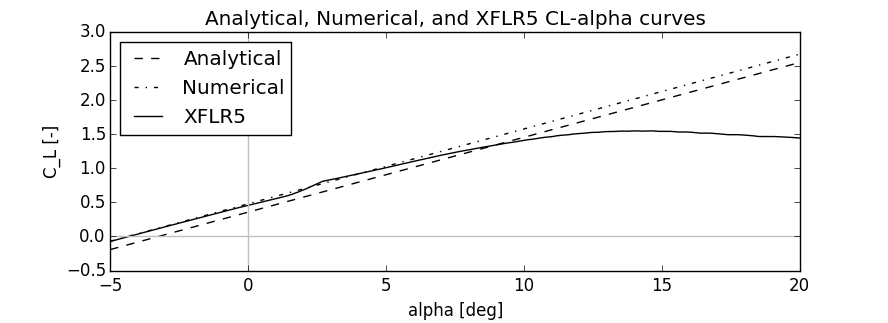
\includegraphics[width=0.8\textwidth]{Aerodynamics/Figures/vercomp}
    \caption{Comparison Between the Analytical, Numerical, and XFLR5 $C_{l}-\alpha$ Curves}
    \label{fig:vercompa}
\end{figure}

%- analytical thin airfoil theory
%- numerical panel method
%- summation of cl over span

%-verified by experience of other people

\nomenclature[B]{$V_{\infty}$}{Undisturbed airflow velocity\nomunit{m/s}}
\nomenclature[B]{$w_{induced}$}{Induced velocity\nomunit{m/s}}
\nomenclature[G]{$\Gamma$}{Vortex strength\nomunit{$m^{2}/s$}}
\nomenclature[B]{$x_{cp}$}{Position of the panel control point as a fraction of the airfoil chord\nomunit{-}}
\nomenclature[B]{$x_{\Gamma}$}{Position of the panel vortex as a fraction of the airfoil chord\nomunit{-}}
 
\subsection{Results Validation}
\label{sub:vval}

\paragraph{Wing} The validation of the wing results begins with the visual inspection of the spanwise lift distribution in order to ensure that it is elliptical (as intended). A comparison between the two is plotted and seen in \autoref{fig:wdist}. It can be seen that the lift distribution closely approximates an elliptical one, therefore this result is considered to be valid.

\begin{figure}[H]
    \centering
    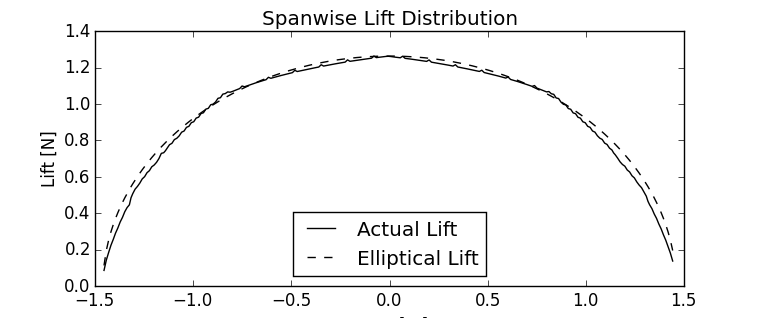
\includegraphics[width=0.8\textwidth]{Aerodynamics/Figures/wdist}
    \caption{Comparison of Actual and Elliptical Lift Distribution}
    \label{fig:wdist}
\end{figure}

The next step is to validate the lift and drag obtained from the SimScale Workbench tool. This is done by comparing the SimScale results to the XFLR5 ones. As seen in the 3D Wing Results in \autoref{sec:aero_wing}, the discrepancy is too large and thus this result is not considered valid. One possible reason for the discrepancy is an improper boundary condition implementation, yet due to resource constraints this claim was not proven. However, since XFLR5 tool was verified, its results are considered to be valid. Therefore the final lift and drag coefficients of the wing are 0.444 and 0.015 respectively.

\paragraph{Tail} The validation of the tail results consists of only a comparison between the SimScale Workbench and XFLR5 results. These forces (as seen in the 3D Tail Results in \autoref{sec:aero_tail}) are similar and in the same order of magnitude as the XFLR results, therefore it is assumed that the setup of the CFD was correct, and the tail lift and drag coefficient is updated to 0.213 and 0.0026 respectively.

\paragraph{Fuselage and Pylons} The validation of the fuselage and pylon results consists of a comparison between the SimScale Workbench and parametric results. 

As seen in the Results in \autoref{sec:aero_fuse}, the fuselage drag force obtained from the SimScale Workbench tool is similar and in the same order of magnitude as the parametric result, therefore it is assumed that the setup of the CFD (including the initial and boundary conditions) was correct and the results are considered valid. Hence, the fuselage drag coefficient is updated to 0.005.

The results in \autoref{sec:aero_pylo} show that the pylon drag force obtained from the SimScale Workbench tool is also similar and in the same order of magnitude as the parametric result, therefore it is assumed that the setup of the CFD was correct and the results are considered valid. Hence, the pylon drag coefficient is updated to 0.00056.

    \chapter{Stability \& Control}
\setlength{\parindent}{15pt}
\label{ch:stab_cont}

The stability and control design and analysis will be explained and presented in this chapter. First of all, \autoref{sec:desi_appr_snc} will clarify the approach followed in order to design and analyse the UAV for stability and control. Secondly, the assumptions used for the analysis are stated in \autoref{sec:assu_snc}. Next, \autoref{sec:anal_snc} explains the methods used to design and analyse the UAV and presents the results of the design and analysis. Finally, the verification and validation of the analysis models, the tools used, and the results are presented in \autoref{sec:veri_vali_snc}.

\section{Design Approach}
\label{sec:desi_appr_snc}

\autoref{fig:StabContFlow} shows the work flow diagram for the stability and control design process. Here, the blue square indicates the design phase for longitudinal stability, the green square indicates the design phase for lateral and directional stability, and the yellow square indicates the design phase comprising the manoeuvres in transition, horizontal, and vertical flight. Different design options can be considered in order to control the UAV and to ensure stability. In the concept selection phase, the decision has been made to have a tail for stability and control surfaces for control in horizontal flight, whereas propellers are used for control and stability in vertical flight. First of all, the tail was sized for longitudinal and lateral control and stability considering the critical case of one engine failure. A tail configuration was selected based on effectiveness and controllability. The required surface area of the vertical and horizontal tail were calculated and the optimal incidence angle of the horizontal tail was found. Simultaneously, the c.g. range needed to be estimated and controlled using the position of the wing as a balancing tool. Secondly, the control surfaces and actuators were sized in order to provide the required angular acceleration in horizontal flight. Thereafter, the propeller power split in order to perform manoeuvres during vertical flight was calculated. Finally, the transition phase was considered and a series of actions was defined in order to have a smooth transition.  %this is an overview of the work flow

The design process of the tail is an iterative process where the global c.g. position and the position of the leading edge of the wing change throughout the design. In order to know the global c.g. the tail needs to be sized. Vice versa, in order to size the tail, the c.g. needs to be known. By using the mass budget and an initial placement of the subsystems, an initial c.g. estimation was made. This estimation was used as a starting point for the tail sizing and wing positioning. Eventually, a more updated c.g. was found using CATIA, so the design could be iterated. Likewise, in order to calculate the position of the leading edge, an initial position needs to be assumed. This leading edge position is needed to calculate the control and stability curves. When the control and stability curves are combined with the c.g.range curves, a new optimal leading edge position can be found. This new leading edge position has to be iterated into the control and stability curves.  %this is some more explanation on the tail iteration

Also the design process of the control principle is an iterative process. Similar to the c.g., the Moment Of Inertia (MOI) changes throughout the design phase. Again, an initial estimation of the MOI was made in order to estimate the required control moments. Next, in order to size the control surfaces, the arm needs to be known which depends on the size of the control surface. Therefore, another iteration process was needed. %here will be some more explanation on the control surface iteration

\nomenclature[A]{MOI}{Moment of Inertia}

\begin{figure}[htb]
    \centering
    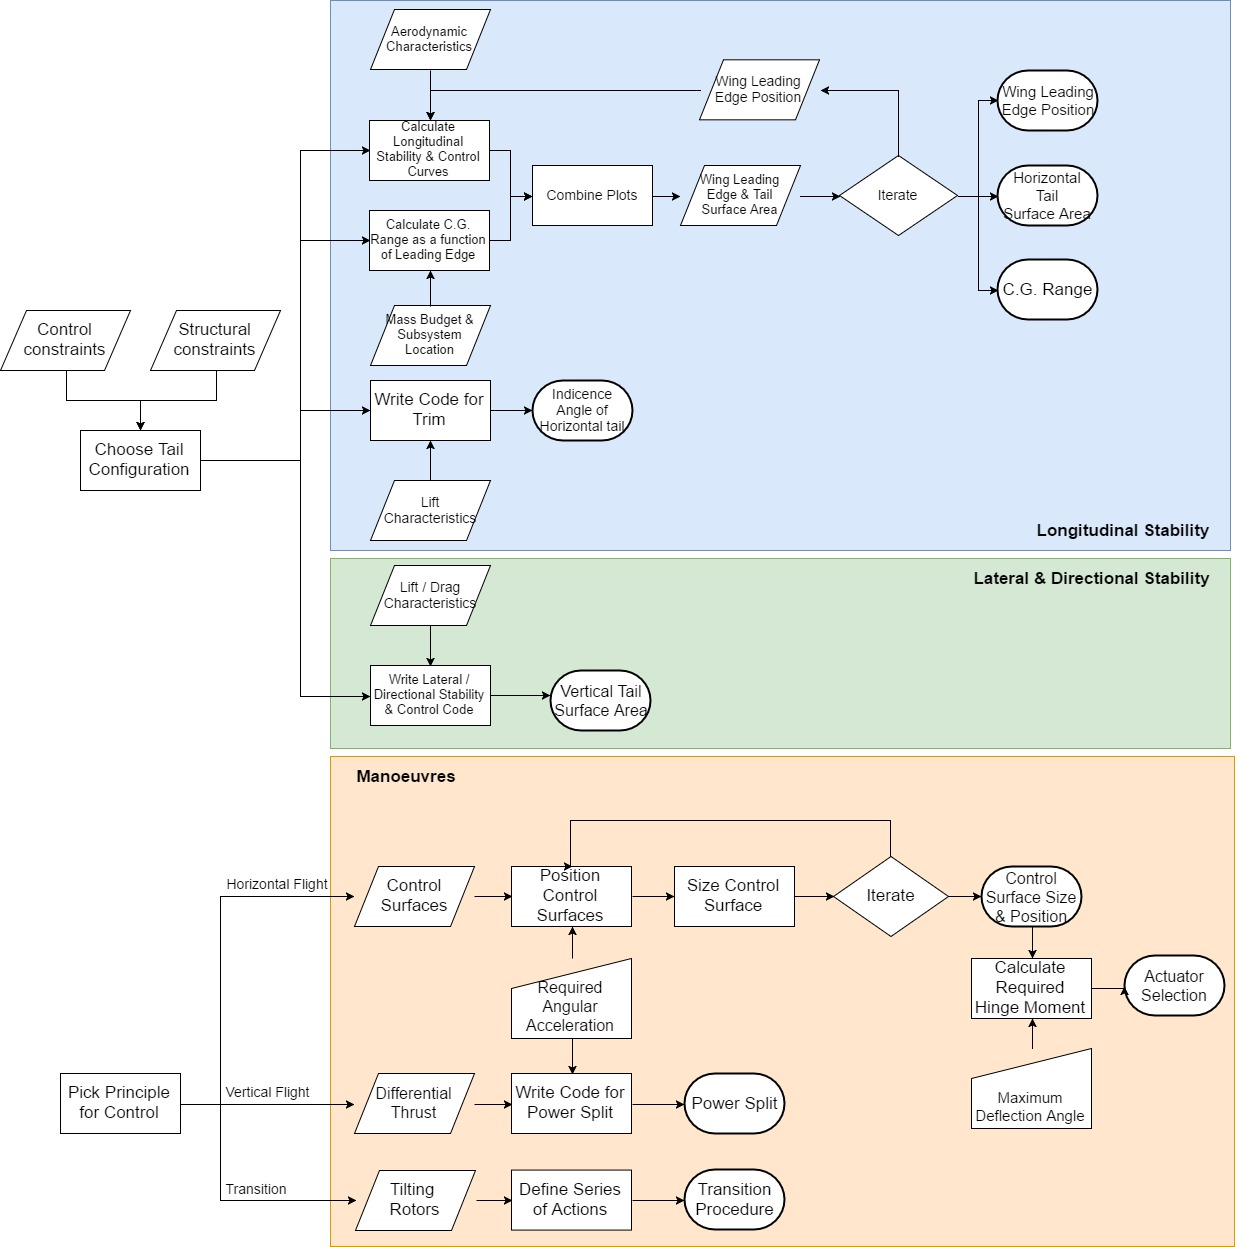
\includegraphics[width=\textwidth]{StabilityandControl/Figures/workflowSNC}
    \caption{Work Flow Diagram for the Stability \& Control Design Process}
    \label{fig:StabContFlow}
\end{figure}

\section{Assumptions}
\label{sec:assu_snc}

\begin{itemize}
    \item It is assumed that the c.g. of the UAV coincides with the a.c. of the wing. With the actual c.g. range located between 0.55 m and 0.74 m from the nose, and the a.c. of the wing located at 0.60 m from the nose, the maximum distance between them is 0.14 m. Therefore, this assumption can be used in the design process without heavily affecting the final results.
    \item It is assumed that the lift coefficient of the horizontal tail during stall, with elevator fully deflected, is equal to -0.8. This value is derived from statistical data for aircraft with adjustable tails \cite{SEAD}.
    \item It is assumed that the resultant force of a control surface goes through half the chord of the control surface. Conventionally, the resulting force is taken through a quarter chord. However, the flow over the control surface is heavily affected by the airfoil in front of it. By assuming the resultant force goes through half the chord, the arm of the force to the hinge is slightly larger than the actual arm. Therefore, the actuators will be slightly over-designed.
    %\item The C$_{m_{ac}}$ of the fuselage and engine nacelles are assumed to be negligible compared to the C$_{m_{ac}}$ of the wing. This assumption is erased because we do include the fuselage contribution
    \item It can be assumed that the downwash at the horizontal tail-plane is negligible. Based on statistical relations based on the horizontal and vertical distance between the wing and tail, the downwash at the tail will have a magnitude of 10$^{-3}$. Hence, this assumption can be considered valid. 
    \item It can be assumed that the tail/wing speed ratio, $\frac{V_h}{V}$, is equal to one. This is a valid assumption since a T-tail is used with sufficient distance between the tail and the vortex shed of the wing. Hence, the perturbations in the flow at the tail caused by the fuselage are negligible. 
    \item It is assumed that the UAV has a plane of symmetry across in the x,y-plane. Hence, the c.g. can be assumed to lie on the plane of symmetry. This assumption can be considered valid since the layout of the plane is symmetrical. Some small deviations may exist because of a non-symmetrical placing of internal components or non-symmetrical payload bay mass distribution.
    \item It is assumed that the fuselage doesn't generate lift. From the CFD analysis done by the aerodynamic department, the fuselage lift coefficient has an order of magnitude of 10$^{-3}$. Therefore, this assumption can be used without affecting the results.
    \item The centre of gravity of the payload bay is assumed to lie between the 10 cm and 50 cm mark measured from the front of the payload bay. This takes into account two loading categories: 1. the need to carry batteries and at the same time having sufficient continuous space for useful payload; 2. the need to carry heavy payloads (i.e. 10 kg) which occupy the entire payload bay. The mass of heavy payloads which occupy the entire payload bay is assumed to be distributed homogeneously throughout the payload volume.
    \item Whilst sizing the vertical tailplane it is assumed that the aerodynamic force induced as a result of side-slip acts perpendicular to the moment arm from the centre of gravity. In reality, the perpendicular component of this aerodynamic force is slightly smaller (scaled with the cosine of the side-slip angle) resulting in a slightly smaller required surface. This assumption therefore makes the calculated surface slightly conservative.
    \item Conservation of momentum and energy laws are assumed to provide sufficient accuracy when calculating the power required during the vertical flight phase. In reality, the motor and propeller efficiency must also be considered. The use of conservative inputs (namely a higher power required to hover) offsets whatever insufficiency the conservation of momentum and energy laws might introduce.
    \item The torque delivered by the motors is assumed to be proportional to the current delivered. It is also assumed that the angular velocity of the motors is proportional to the voltage applied. In reality this is loosely accurate, however, it not entirely correct to assume both torque and angular velocity vary linearly. This does not affect the required power splits, however, the motor-propeller combination must be tested experimentally to see how the output power varies with varying current and voltage.
\end{itemize}

\section{Analysis}
\label{sec:anal_snc}
This section shows the methods used to analyse and design the UAV for stability and control, and presents the final results. 

\subsection{Tail Configuration}
First of all, a tail configuration was picked based on the effectiveness, structural weight, and controllability of the tail-planes. Since downwash caused by the vortex of the wing reduces the effectiveness of the tail, a horizontal tailplane located outside of the downwash is preferred. Furthermore, it would be favourable to have tailplanes where roll and yaw, and longitudinal and lateral control are separated from each other. The structural weight of the tail was also taken into account when choosing a tail configuration. For example, a V-tail has a reduced amount of components. 
A T-tail was chosen as the final tail configuration mainly because downwash can be completely neglected and the control surfaces can be completely separated. At the same time, the structural weight can stay within the budget.

\begin{equation}
\label{eq:trimbla}
    C_{L_{h}} = C_{L_{cruise}}\frac{S}{S_h}\frac{(x_{c.g.}-x_{a.c._{w}})}{(x_{a.c._{h}}-x_{c.g.})}
\end{equation}

Next, the incidence angle of the horizontal tailplane was calculated in order to be trimmed without the need of deflecting the elevator. The required tail lift coefficient was calculated for cruise conditions using \autoref{eq:trimbla} which is derived from the trim equation. The optimal incidence angle can be found by finding the corresponding angle of attack in the $C_L$-$\alpha$ curve of the tail.

\subsection{Longitudinal Stability \& Control}
The UAV is required to be longitudinally statically stable. This means that it is able to react to a change in the angle of attack by generating an opposite pitching moment to restore the former state of equilibrium. In order to achieve stability, the c.g. should be positioned in front of the neutral point. The position of the neutral point is dependent on the ratio of wing/tail surface areas. When taking into account a Safety Margin (SM) of 0.05\footnote{AE3211-I Lecture 5 - Requirement Analysis and Design principles for A/C stability \& control (Part 1)}, the maximum position of the c.g. (in order to be stable) can be calculated as a function of the wing/tail surface ratio, as can be seen in \autoref{eq:stabSM}. In this equation, a macron (the bar on top of a symbol) indicates it is divided by the mean aerodynamic chord of the wing. The downwash is assumed to be zero and wing/tail speed ratio can be assumed to be equal to one since a T-tail configuration is used. The distance between the wing and tail, $l_h$, can be estimated by assuming an initial position of the leading edge of the wing and iterating it. The other parameters are aerodynamic characteristics.

\begin{equation}
\label{eq:stabSM}
    \bar{x}_{c.g._{max}}=\bar{x}_{a.c.}+\frac{C_{L_{\alpha_h}}}{C_{L_{\alpha_{A-h}}}}\Big(1-\frac{d\epsilon}{d\alpha}\Big)\frac{S_h l_h}{S\bar{c}}\Big(\frac{V_h}{V}\Big)^2-SM
\end{equation}

\nomenclature[B]{$x_{c.g._{max}}$}{Maximum centre of gravity position from the nose \nomunit{m}}
\nomenclature[B]{$x_{c.g._{min}}$}{Minimum centre of gravity position from the nose \nomunit{m}}
\nomenclature[B]{$x_{a.c.}$}{Position of the aerodynamic centre of the wing from the nose \nomunit{m}}
\nomenclature[B]{$C_{L_{\alpha_h}}$}{Lift slope coefficient of the tail \nomunit{-}}
\nomenclature[B]{$C_{L_{\alpha_{A-h}}}$}{Lift slope coefficient of the aircraft minus tail \nomunit{-}}
\nomenclature[B]{$\frac{d\epsilon}{d\alpha}$}{Downwash \nomunit{-}}
\nomenclature[B]{$S$}{Wing surface area \nomunit{m$^2$}}
\nomenclature[B]{$S_h$}{Tail surface area \nomunit{m$^2$}}
\nomenclature[B]{$l_h$}{Distance between the a.c. of the wing and the a.c. of the tail \nomunit{m}}
\nomenclature[B]{$\bar{c}_w$}{Mean aerodynamic chord of the wing \nomunit{m}}
\nomenclature[B]{$\frac{V_h}{V}$}{Tail/wing speed ratio \nomunit{-}}
\nomenclature[A]{SM}{Safety Margin}

Additionally, the UAV is required to be controllable. An aircraft is said to be controllable when it is able to be trimmed for a certain aircraft configuration. In other words, a combination of wing and tail lift coefficient should result in a zero total aircraft moment coefficient. In order to achieve controllability, the c.g. has to be positioned behind a certain limit point. This point can be found as a function of the wing/tail surface area by using the trim equation. Here the moment generated by the wing around the c.g. has to be equal to the moment generated by the tail around the c.g.. When rewriting this equation, the minimum position of the c.g. (in order to be controllable) can be calculated as a function of the wing/tail surface area, as can be seen in \autoref{eq:stabeq}. Again, the wing/tail speed ratio can be assumed to be equal to one. The distance between the wing and tail can be estimated and iterated. The aerodynamic characteristics are input in the remaining parameters.

\begin{equation}
\label{eq:stabeq}
    \bar{x}_{c.g._{min}}=\bar{x}_{a.c.}-\frac{C_{m_{a.c.}}}{C_{L_{A-h}}}+\frac{C_{L_{h}}}{C_{L_{A-h}}}\frac{S_h l_h}{S \bar{c}}\Big(\frac{V_h}{V}\Big)^2
\end{equation}

These two equations can be plotted with the c.g. measured from the leading edge divided by the mean aerodynamic chord on the x-axis, and the wing/tail surface area on the y-axis. This plot is called the scissor plot, presented as the blue curves in \autoref{fig:scissor}. In between the two curves lies the region where, if the c.g. is positioned there, the aircraft is stable and controllable. The position of the wing is used as a balancing tool in order to get the actual c.g. range shifted to the optimal position in order to have the lowest wing/tail ratio. Visually, this means that a plot of the c.g. range as a function of the leading edge has to be combined and shifted vertically to the scissor plot until the range of the c.g. plot matches with the width of the scissor plot.

\begin{figure}[htb]
    \centering
    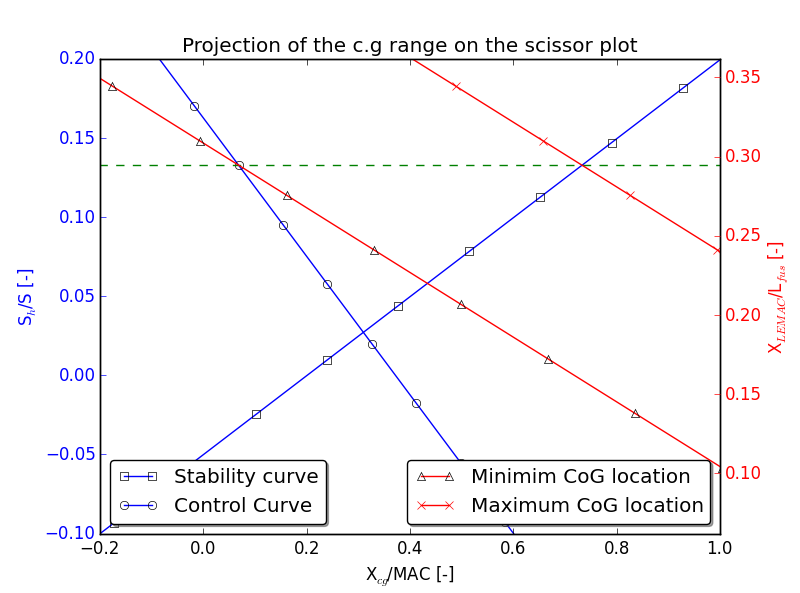
\includegraphics[width=0.7\textwidth]{StabilityandControl/Figures/Scissor}
    \caption{Projection of the C.G. Range on the Scissor Plot}
    \label{fig:scissor}
\end{figure}

\nomenclature[B]{$x_{LE}$}{Leading edge position of the wing from the nose}
\nomenclature[B]{$L_{fus}$}{Fuselage length}

Now the c.g. plot needs to be calculated. Here, the c.g. range is plotted with the c.g. measured from the leading edge divided by the mean aerodynamic chord on the x-axis, and the wing leading edge divided by the length of the fuselage on the y-axis. Hence, the x-axes of both the scissor and c.g. plots are the same. In order to calculate the c.g. range, \autoref{eq:c.g.r} is used. Here, $m_i$ is the mass of a subsystem, $x_i$ is the c.g. of the subsystem, and n is the number of subsystems. Since the c.g. of the payload bay has a minimum and a maximum value, a range of c.g. values is found. Furthermore, the c.g. value depends on the x-location of the wing, which depends on the position of the leading edge of the wing. Hence, the c.g. range can be expressed as a function of the wing leading edge over the length of the fuselage. The curves for the maximum and minimum c.g. ranges are presented as the red curves in \autoref{fig:scissor}.

\begin{equation}
\label{eq:c.g.r}
    x_{c.g.} = \frac{\sum_{i=1}^{n} {x_i\cdot m_i}}{\sum_{i=1}^{n_i} {m_i}}
\end{equation}

By shifting the c.g. plot over the scissor plot, one can see in \autoref{fig:scissor} that an optimal value for the wing/tail ratio, and leading edge over fuselage length ratio can be found. This is indicated by the green dotted line extended between both y-axes. The final results are presented in \autoref{tab:scissorres}. The final values used to calculate the total c.g. position can be found in \autoref{tab:cgbreakdown}.

\begin{table}[htb]
\centering
\caption{Results of the Scissor and c.g. Plot}
\label{tab:scissorres}
\begin{tabular}{lll}
\toprule
\textbf{Parameter} & \textbf{Value} & \textbf{Unit} \\ \midrule
$x_{cg_{min}}$     & 0.55           & m             \\ \hdashline
$x_{cg_{max}}$     & 0.74           & m             \\ \hdashline
$x_{LE}$           & 0.53           & m             \\ \hdashline
$S_h$              & 0.106          & m$^2$      \\  \bottomrule
\end{tabular}
\end{table}

\subsection{Lateral/Directional Stability \& Control}

In this section, the lateral and directional stability and control of the UAV is analysed. In order to achieve this, the vertical tail area of the system has to be designed. Using wing mounted engines, the critical design case for vertical tail sizing is obtained in the one-engine-out condition. In this case, the remaining engine creates a yaw-moment which needs to be counteracted using the vertical tailplane. Although a rudder deflection might also be used for this, the moment should only be based on the vertical tailplane, as directional yaw control of the aircraft in both directions is still needed and achieved using rudder deflections.

First, a necessary yaw angle at which equilibrium is achieved needs to be defined. It was assumed, that in one engine out condition, equilibrium will be obtained at a yaw angle of 5$^\circ$. Then, the UAV velocity will be reduced to maximum range speed, $V_{range} = 27 \frac{m}{s}$, in order to be able to fly to the best landing location. In case the engine fails at a lower velocity, the drag will be lower and in turn less thrust is required. This will reduce the yaw moment and thus flying at lower velocities will also be possible. Using aerodynamic properties, the thrust required for the remaining engine is now obtained with \autoref{eq:drag_vertical}. 

\begin{equation}
    T = C_D\cdot\frac{1}{2}\cdot\rho\cdot V^2_{range}\cdot S
    \label{eq:drag_vertical}
\end{equation}

Then, considering the fact that the engines are all mounted at the same distance $y_{engine}$ from the centre of gravity, the yaw moment created by the one-engine-out condition is obtained using $M = T\cdot y_{engine}$. This yaw moment has to be counteracted by the vertical tailplane at an angle of side-slip of $\beta = 5^\circ$. As the moment arm, airfoil, velocity, and the sweep angle of the vertical tailplane are known, the required surface area can be calculated using \autoref{eq:surf_area_vert}.

\nomenclature[B]{$y_{engine}$}{Distance between engines and centre of gravity along the wingspan \nomunit{m}}

\begin{equation}
    S_{vertical} = \frac{2\cdot M_{yaw}}{l_v\cdot C_{L_{\beta_v}}\cdot \beta\cdot\rho\cdot (V_{range}\cdot cos(\lambda_{v}))^2}
    \label{eq:surf_area_vert}
\end{equation}

In \autoref{eq:surf_area_vert}, $M_{yaw}$ is the yaw moment generated by the engine, $l_v$ the distance between the centre of gravity and the aerodynamic centre of the vertical tailplane, $\lambda_v$ the sweep angle of the vertical tailplane, and $C_{L_{\beta_v}}$ the lift coefficient/sweep angle slope obtained using an XFLR5 analysis. For lateral stability, the vertical tail must have a surface area of 0.026 $m^2$.
\nomenclature[B]{$M_{yaw}$}{Yaw moment \nomunit{Nm}}
\nomenclature[B]{$l_v$}{Distance between centre of gravity of the UAV and the aerodynamic centre \nomunit{m}}
\nomenclature[G]{$\lambda_v$}{Sweep angle of the vertical tailplane \nomunit{rad}}
\nomenclature[B]{$C_{L_{\beta_v}}$}{Vertical tailplane lift coefficient slope \nomunit{-}}




%Creates roll moment --> counteracted using ailerons 



\subsection{Control Surfaces}

In this section the size and position of the control surfaces are determined. These are ailerons for roll control, an elevator for pitch control, and a rudder for yaw control. Then, the hinge moment is calculated in order to select suitable servos. 

The design of the control surfaces is dependent on the angular accelerations required. From requirements SUB-W-7.3, SUB-T-2.2, and SUB-T-2.3, the following angular accelerations are defined.

\begin{equation*}
    \alpha_{roll} = \alpha_{pitch} = 45 \frac{^\circ}{s^2} \quad \alpha_{yaw} = 6 \frac{^\circ}{s^2}
\end{equation*}

\nomenclature[G]{$\alpha_{roll}$}{Angular roll acceleration \nomunit{rad/s$^2$}}
\nomenclature[G]{$\alpha_{pitch}$}{Angular pitching acceleration \nomunit{rad/s$^2$}}
\nomenclature[G]{$\alpha_{yaw}$}{Angular yaw acceleration \nomunit{rad/s$^2$}}

Using the moments of inertia, the torque required is obtained using \autoref{eq:newton2}. These torques have to be created by the control surfaces and hence depend strongly on the physical location of the control surfaces. The elevator is located at the trailing edge of the horizontal tailplane. The ailerons are positioned as far away from the fuselage as possible in order to maximise the moment arm. In order to avoid twisting the control surfaces themselves, they can not be positioned at the wing tips. Therefore, they will be positioned just before the start of the wing twist. The rudder is located at the trailing edge of the vertical tailplane. The locations of the control surfaces lead to the moment arms.

\begin{equation}
    T = I \cdot \alpha
    \label{eq:newton2}
\end{equation}

With the moment arms and the torque required, one can calculate the required force for the surface. The force generated by deflecting the surfaces to an angle of $\delta$ is given by \autoref{eq:cont_forc}.

\begin{equation}
    F = C_{n_{\delta}}\cdot \delta\cdot\frac{1}{2}\cdot\rho\cdot V^2 \cdot S
    \label{eq:cont_forc}
\end{equation}

In \autoref{eq:cont_forc}, $C_{n_{\delta}}$ is obtained using an XFLR5 analysis. In order to size the control surfaces, stall speed is assumed. This ensures that the surface is capable of providing enough force for the whole speed range. Comparing control surface deflection angles of different aircraft, the following maximum deflection angles were defined: 

\nomenclature[B]{$C_{n_{\delta}}$}{Normal force gradient \nomunit{-}}
\nomenclature[G]{$\delta$}{Control surface deflection angle \nomunit{deg}}
\begin{equation*}
    \delta_{elevator_{max}} = 28^\circ\quad\delta_{rudder_{max}} = 25^\circ\quad\delta_{aileron_{max}} = 30 ^\circ
\end{equation*}

Using these parameters, it is now possible to calculate the surface area of the different control surfaces by rearranging \autoref{eq:cont_forc}. 
Now, the aileron chord is assumed to be 20\% of the wing chord, elevator span to be 70\% of the horizontal tailplane span, and rudder span to be 90\% of the vertical tailplane span. This makes it possible to calculate the different dimensions for the surface area. 

Using the dimensions of the different control surfaces, an appropriate servo has to be chosen. For this, it is necessary to calculate the torque required to maintain a the maximum certain deflection. 

\begin{figure}[htb]
    \centering
    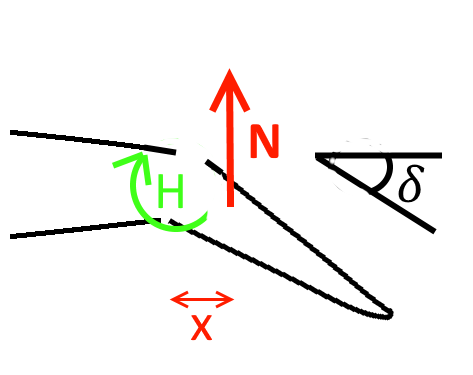
\includegraphics[scale=1]{./StabilityandControl/Figures/hinge}
    \caption{Hinge Moment Created by the Control Surface Force}
    \label{fig:hing}
\end{figure}

As can be seen in \autoref{fig:hing}, the hinge moment created by the normal force N is dependant on the aerodynamic centre of the control surface. For calculation purposes it is assumed that the force acts halfway through the chord. The actual hinge moment will be lower as the aerodynamic centre is in general located at the quarter-point of the chord. Then for the sizing, worst case scenario is assumed, meaning flying at maximum speed of 200 $\frac{km}{s}$ and deflecting the control surface to maximum deflection. The control force is then calculated using \autoref{eq:cont_forc}, which, multiplied by the moment arm, gives the hinge moment. The final control surface results are illustrated in \autoref{tab:cont_surf}.

\nomenclature[B]{$N$}{Normal force \nomunit{N}}

\begin{table}[htb]
    \centering
    \caption{Control Surface Properties}
    \label{tab:cont_surf}
    \begin{tabular}{lcccc}
      \toprule
        & Span [cm]& Chord [cm]& Surface Area [$cm^2$] & Maximum Hinge Moment [Ncm] \\
      \midrule
      Aileron & 17.1 & 3.69 & 63.1 &23\\\hdashline
      Elevator & 47.2 &2.89& 136  &36\\\hdashline
      Rudder & 16.3 & 2.67 & 43.4 &12\\\bottomrule
    \end{tabular}
\end{table}

Four SAVÖX SC-0254MG servos are used for both ailerons, the elevator and the rudder. They are able to deliver a torque of 62 Ncm at minimum power consumption. \footnote{\url{https://www.hacker-motor-shop.com/Servos/Savoex-Servos/Servos-Flugmodelle/Servo-SAVOeX-SC-0254MG.htm?SessionId=&a=article&ProdNr=80101005&p=6264}, Accessed 22-06-2017}

\subsection{Vertical Flight Manoeuvres} %This is subject to change

During the vertical flight phase of the the UAV various manoeuvres have to be considered, namely pitch, roll and yaw, all of which are achieved purely through varying the thrust level of the four propellers. By varying the power applied to motor couples the required moments about the axis around which the manoeuvre takes place can be produced. In this section the power required to achieve specified angular accelerations about the three axes will be characterised. However it is necessary to first define the locations of the four motors with respect to the centre of gravity. It is important to note that the conventional body axis system with its origin located at the centre of gravity is used in this section; i.e. the $x$-axis points in the direction of the nose, the $y$-axis runs along the right wing and the $z$-axis completing the system. 

\paragraph{General Layout of Motors}
As explained in \autoref{ch:powe_prop} the front motor-propeller combination was chosen to provide most of the thrust during the vertical flight phase whereas the aft motor-propeller combination was chosen to propel the UAV during horizontal flight. This results in the distance from the centre of gravity to the front motors being smaller than the distance from the centre of gravity to the aft motors in the longitudinal direction. For control reasons and simplicity's sake it is beneficial if the lateral and longitudinal distances between the motors are equal.

It was also important to define the direction of rotation of the propellers in order to perform calculations for the required torque about $z$-axis for yaw manoeuvres. The direction of rotation of the motors is chosen such that during hovering and vertical climb the total torque around the centre of gravity is zero as well as such that yaw manoeuvres can be performed. Both conditions are satisfied when the front motors rotate in opposite directions as well as when motors diagonally opposite rotate in the same direction. The following configuration with respect to the centre of gravity is assumed for further calculations.

\begin{figure}[htb]
    \centering
    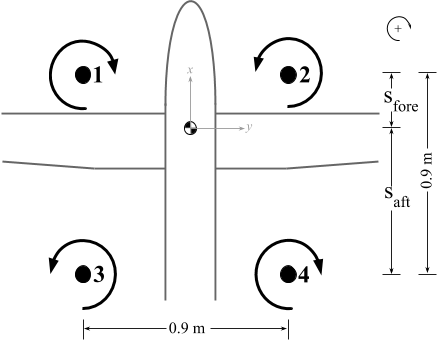
\includegraphics[width=0.6\textwidth]{StabilityandControl/Figures/Template_layout}
    \caption{Configuration with respect to the Centre of Gravity}
    \label{fig:layout}
\end{figure}

By equating the moment created by the front motors to the moment created by the aft motors around the $y$-axis the distances from the centre of gravity to the front and aft motors can be calculated. Values for S$_{fore}$ and S$_{aft}$ are presented in \autoref{tab:dist_cog_motors} below.

\begin{table}[H]
    \centering
    \caption{Table of the Distances of the Motors from the CoG}
    \begin{tabular}{lcc}
        \toprule
        \textbf{Distance} & \textbf{from min CoG [m]} & \textbf{from max CoG [m]} 
        \\ \midrule
        S$_{fore}$        & 0.229                     & 0.390
        \\ \hdashline
        S$_{aft}$         & 0.771                     & 0.610
        \\ \bottomrule
    \end{tabular}
    \label{tab:dist_cog_motors}
\end{table}

\paragraph{Pitch}
In order to perform a pitch up or down manoeuvre during vertical flight a change in moment around the $y$-axis has to be induced by the motors. As stipulated by requirement \textbf{SUB-PR-3.5} the propulsion subsystem shall be capable of providing an angular acceleration, $\alpha_{pitch}$ about the $y$-axis of 0.8 rad/s$^2$. The moment required to deliver the stipulated angular acceleration is defined as the follows:

\begin{equation}
\label{eq:requ_mome_pitc}
M_{pitch} = I_{yy} \cdot \alpha_{pitch}
\end{equation}

\nomenclature[B]{$M_{pitch}$}{Moment required for pitch manoeuvre \nomunit{N$\cdot$m}}
\nomenclature[B]{$I_{yy}$}{Moment of Inertia around the $y$-axis \nomunit{kg$\cdot$m$^2$}}

The required moment to deliver the angular pitching acceleration outlined by the requirement can then be translated into the change in thrust required ($\Delta$T) of the motor-propeller couples by dividing by the moment arms presented in \autoref{tab:dist_cog_motors}. During pitch manoeuvres it is assumed that the required moment will always be delivered by increasing the thrust of the front or aft motors-couples rather than increasing one and simultaneously decreasing the other. This is done as it is assumed that unless the UAV is in transition, the rotation of the motors will be kept to a minimum. Because of this, as the pitch motion is initiated the effective vertical force of the propellers decreases with the cosine of the angle of rotation. If the overall power was to be kept constant during pitching (by increasing either the fore or aft motors and decreasing the opposite) altitude will be lost. The loss of altitude can be mitigated by simply delivering the entire required moment with the increase of thrust of the fore \textbf{or} aft motor-propeller couples (depending on the direction of pitch required) rather than splitting the required moment over both the fore and aft motors.

\begin{figure}[H]
    \centering
    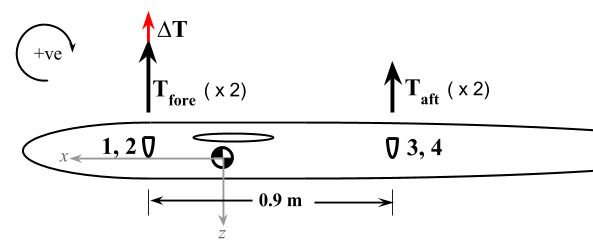
\includegraphics[width=0.6\textwidth]{StabilityandControl/Figures/Side_view_control.png}
    \caption{Side View Schematic of Pitch}
    \label{fig:schematic_side}
\end{figure}

For a pitch up manoeuvre (positive pitch) with an angular acceleration of 0.8 rad/s$^2$ the power required is calculated using equation \autoref{eq:powe_requ_pitch}. Note that this procedure is the same for a pitch down manoeuvre apart from the fact that the aft motors will be responsible for the manoeuvre as opposed to the front motors.

\begin{equation}
\label{eq:powe_requ_pitch}
P_{req} = \sqrt{\frac{(T_{fore}+\frac{\Delta T}{2})^{3}}{2 \cdot \rho \cdot A_{fore}}}
\end{equation}

Where T$_{fore}$ is the thrust of the front motor-propeller couples during hovering. The change in power required in order to deliver the required moment is therefore the difference between the power required to hover and the power required calculated above in \autoref{eq:powe_requ_pitch}.

Power can also be defined as the product of the torque delivered and the angular velocity and so by increasing the angular velocity of the propeller the power required to perform the pitch manoeuvre can be achieved. The relationship between power, torque and angular velocity is given by the following equation

\begin{equation}
\label{eq:powe_torq_angu_velo}
P = \tau \cdot \omega
\end{equation}

By increasing the voltage supplied to the motor (also increasing the power for a fixed current) the angular velocity can be increased as the angular velocity of the motor proportional to the voltage.

\paragraph{Roll}
In order to perform a pitch up or down manoeuvre during vertical flight a change in moment around the $x$-axis has to be induced by the motors. Essentially the same procedure as laid out in the above section can be employed however it is slightly more complicated given the fact that the fore and aft motors are not the same. 

\begin{figure}[H]
    \centering
    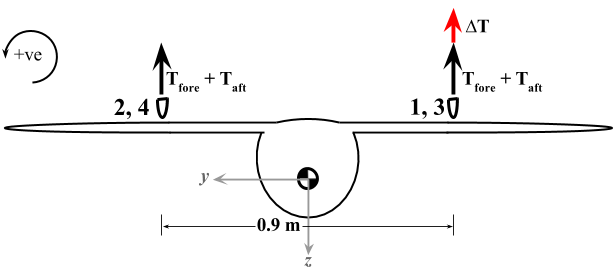
\includegraphics[width=0.6\textwidth]{StabilityandControl/Figures/Front_view_control.png}
    \caption{Front View Schematic of Roll}
    \label{fig:schematic_front}
\end{figure}

The moment required to achieve the angular acceleration stipulated by requirement \textbf{SUB-PR-3.4} is given by the equation below.

\begin{equation}
\label{eq:requ_mome_roll}
M_{roll} = I_{xx} \cdot \alpha
\end{equation}

\nomenclature[B]{$M_{roll}$}{Moment required for roll manoeuvre \nomunit{N$\cdot$m}}
\nomenclature[B]{$I_{xx}$}{Moment of Inertia around the $x$-axis \nomunit{kg$\cdot$m$^2$}}

By dividing the roll moment by the $y$-distance from the centre of gravity to the motors the combined required change in thrust ($\Delta$T) is obtained. Because the fore and aft motors are different, in order to achieve pure roll the same ratio as during hovering of thrust produced by the front propeller to the thrust produced by the aft propellers must be used. 
For a positive roll manoeuvre the power required to deliver this thrust is characterised by the following equation.

\begin{minipage}{0.48\textwidth}
    \begin{equation}
        P_{req_{1}} = \sqrt{\frac{(T_{fore}+(\frac{\Delta T}{2} \cdot \frac{T_{ratio}}{T_{ratio} + 1}))^{3}}{2 \cdot \rho \cdot A_{fore}}}
        \label{eq:powe_requ_moto_1_roll}
    \end{equation}
\end{minipage}%
\begin{minipage}{0.48\textwidth}
    \begin{equation}
        P_{req_{3}} = \sqrt{\frac{(T_{fore}+(\frac{\Delta T}{2} \cdot \frac{1}{T_{ratio} + 1}))^{3}}{2 \cdot \rho \cdot A_{fore}}}
        \label{eq:powe_requ_moto_3_roll}
    \end{equation}
\end{minipage}

Where subscripts 1 \& 3 represent motor 1 and 3 from \autoref{fig:layout} respectively as those are the motors responsible for a positive roll moment. Again, the required moment is not split across the $x$-axis in order to mitigate altitude loss because of effective vertical thrust decreasing with the cosine of angle of rotation. The change in power required for motors 1 and 3 during a positive roll manoeuvre can be achieved by increasing the angular velocity of the motors which in turn can be done by increasing the applied voltage. 

\paragraph{Yaw}
Positive or negative yaw manoeuvres during vertical flight can be performed by altering the torques of the motors. Each motor exerts a certain torque on the entire body due its rotation and this phenomenon can be exploited to perform manoeuvres. As depicted in \autoref{fig:layout} motors 1 and 4 rotate in the same direction as do motors 2 and 3 and so during yaw manoeuvres these pairs of motors will work together the provide the required moment. As stipulated by requirement \textbf{SUB-PR-3.6} the propulsion subsystem shall be capable of providing an angular acceleration, $\alpha_{yaw}$ about the $z$-axis of 0.1 rad/s$^2$. The moment required to deliver the required angular acceleration is characterised by the following equation.


\begin{equation}
\label{eq:requ_mome_yaw}
M_{yaw} = I_{zz} \cdot \alpha_{yaw}
\end{equation}

\nomenclature[B]{$M_{yaw}$}{Moment required for yaw manoeuvre \nomunit{N$\cdot$m}}
\nomenclature[B]{$I_{zz}$}{Moment of Inertia around the $z$-axis \nomunit{kg$\cdot$m$^2$}}

This moment can be achieved by altering the torque of the motors. During hovering, the torque delivered by each motor can simply be calculated by dividing the power required to hover by the nominal angular velocity of the motors during hovering. 

\begin{figure}[htb]
    \centering
    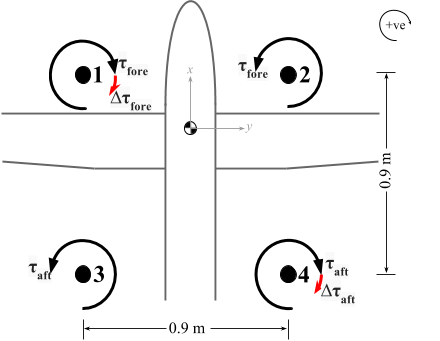
\includegraphics[width=0.6\textwidth]{StabilityandControl/Figures/Top_view_control.png}
    \caption{Top View Schematic of Roll}
    \label{fig:schematic_top}
\end{figure}

For a positive yaw manoeuvre the change in torque ($\Delta \tau$) required is split up over motor 1 and 4 (from \autoref{fig:layout}). This torque is split up according to the ratio of torque of motor 1 to torque of motor 4 (please note that for a negative yaw manoeuvre the same procedure is applied except the opposite motor pairs will be increasing or decreasing power respectively). The change in power ($\Delta$P) of the motors delivering the manoeuvre (i.e. motors 1 and 4) as a result of the increase in torque required can be calculated by multiplying the torque required of each motor with their respective angualar velocities as shown in Equations \ref{eq:powe_requ_moto_1_yaw} \& \ref{eq:powe_requ_moto_4_yaw}. \newline

\begin{minipage}{0.48\textwidth}
    \begin{equation}
    \label{eq:powe_requ_moto_1_yaw}
    \Delta P = \Delta \tau_1 \cdot \omega_1
    \end{equation}  
\end{minipage}%
\begin{minipage}{0.48\textwidth}
    \begin{equation}
    \label{eq:powe_requ_moto_4_yaw}
    \Delta P = \Delta \tau_4 \cdot \omega_4
    \end{equation}
\end{minipage}
\newline

In order to maintain altitude this change in power (increase) must be countered by a decrease in power from the other two motors, namely motors 2 and 3. The increase in power required of motor 1 (from \autoref{eq:powe_requ_moto_1_yaw}) needs to be subtracted from the power required of motor 2 to hover and likewise the increase in power required of motor 4 (from \autoref{eq:powe_requ_moto_4_yaw}) needs to be subtracted from the power required of motor 3 to hover.

In order to ensure that the required torque is delivered, the positive change in power required of motors 1 and 4 should be achieved by increasing the current delivered to the said motors as torque is proportional to current. The decrease in power of the remaining two motors can simply be achieved by decreasing the respective angular velocities by lowering the applied voltage.

\paragraph{Results}
The following tables breaks down the required power to perform the three outlined manoeuvres.


\begin{table}[H]
\centering
\caption{Table of Power Required for Motors 1 \& 2}
\label{tab:powe_requ_moto_1_2}
\begin{tabular}{lll|cc|cc|}
\cline{4-7}
                           &                            &                                  & \multicolumn{2}{c|}{\textbf{Motor 1}}    & \multicolumn{2}{c|}{\textbf{Motor 2}}    \\ \cline{4-7} 
                           &                            &                                  & \textbf{c.g.$_{min}$}    & \textbf{c.g.$_{max}$}    & \textbf{c.g.$_{min}$}    & \textbf{c.g.$_{max}$}    \\ \hline
\multicolumn{1}{|l}{\textbf{Hover}} & \multicolumn{1}{l|}{}      & P$_{req}$ {[}W{]}                & 2423.89        & 1553.15        & 2423.89        & 1553.15        \\ \hline
\multicolumn{1}{|l}{\textbf{Pitch}} & \multicolumn{1}{l|}{+ve}   & P$_{req}$ {[}W{]}                & 2519.14        & 1599.12        & 2519.14        & 1599.12        \\ \hdashline
\multicolumn{1}{|l}{}      & \multicolumn{1}{l|}{$-$ve} & P$_{req}$ {[}W{]}                & 2423.89        & 1553.15        & 2423.89        & 1553.15        \\ \hline
\multicolumn{1}{|l}{\textbf{Roll}}  & \multicolumn{1}{l|}{+ve}   & P$_{req}$ {[}W{]}                & 2472.59        & 1584.35        & 2423.89        & 1553.15        \\ \hdashline
\multicolumn{1}{|l}{}      & \multicolumn{1}{l|}{$-$ve} & P$_{req}$ {[}W{]}                & 2423.89        & 1553.15        & 2472.59        & 1584.35        \\ \hline
\multicolumn{1}{|l}{\textbf{Yaw}}   & \multicolumn{1}{l|}{+ve}   & P$_{req}$ {[}W{]}                       & 2774.47        & 1806.77        & 2073.30        & 1299.52        \\ \hdashline
\multicolumn{1}{|l}{}      & \multicolumn{1}{l|}{}      & ($\Delta \tau$, $\Delta \omega$) & (0.74 , 0.0)   & (0.54 , 0.0)   & (0.0 , -68.16) & (0.0 , -76.95) \\ \hdashline
\multicolumn{1}{|l}{}      & \multicolumn{1}{l|}{$-$ve} & P$_{req}$ {[}W{]}                       & 2073.30        & 1299.52        & 2774.47        & 1806.77        \\ \hdashline
\multicolumn{1}{|l}{}      & \multicolumn{1}{l|}{}      & ($\Delta \tau$, $\Delta \omega$) & (0.0 , -68.16) & (0.0 , -76.95) & (-0.74 , 0.0)  & (-0.54 , 0.0)  \\ \hline
\end{tabular}
\end{table}

\begin{table}[H]
\centering
\caption{Table of Power Required for Motors 3 \& 4}
\label{tab:powe_requ_moto_3_4}
\begin{tabular}{lll|cc|cc|}
\cline{4-7}
                           &                            &                                  & \multicolumn{2}{c|}{\textbf{Motor 3}}      & \multicolumn{2}{c|}{\textbf{Motor 4}}      \\ \cline{4-7} 
                           &                            &                                  & \textbf{c.g.$_{min}$}    &\textbf{ c.g.$_{max}$}     & \textbf{c.g.$_{min}$}     & \textbf{c.g.$_{max}$}     \\ \hline
\multicolumn{1}{|l}{\textbf{Hover}} & \multicolumn{1}{l|}{}      & P$_{req}$ {[}W{]}                & 661.58          & 1575.57         & 661.58          & 1575.57         \\ \hline
\multicolumn{1}{|l}{\textbf{Pitch}} & \multicolumn{1}{l|}{+ve}   & P$_{req}$ {[}W{]}                & 661.58          & 1575.57         & 661.58          & 1575.57         \\ \hdashline
\multicolumn{1}{|l}{}      & \multicolumn{1}{l|}{$-$ve} & P$_{req}$ {[}W{]}                & 693.91          & 1633.53         & 693.91          & 1633.53         \\ \hline
\multicolumn{1}{|l}{\textbf{Roll}}  & \multicolumn{1}{l|}{+ve}   & P$_{req}$ {[}W{]}                & 674.88          & 1607.22         & 661.58          & 1575.57         \\ \hdashline
\multicolumn{1}{|l}{}      & \multicolumn{1}{l|}{$-$ve} & P$_{req}$ {[}W{]}                & 661.58          & 1575.57         & 674.88          & 1607.22         \\ \hline
\multicolumn{1}{|l}{\textbf{Yaw}}   & \multicolumn{1}{l|}{+ve}   & P$_{req}$ {[}W{]}                       & 565.89          & 1318.28         & 757.27          & 1832.86         \\ \hdashline
\multicolumn{1}{|l}{}      & \multicolumn{1}{l|}{}      & ($\Delta \tau$, $\Delta \omega$) & (0.0 , -113.60) & (0.0 , -128.25) & (0.12 , 0.0)    & (0.33 , 0.0)    \\ \hdashline
\multicolumn{1}{|l}{}      & \multicolumn{1}{l|}{$-$ve} & P$_{req}$ {[}W{]}                       & 757.27          & 1832.86         & 565.89          & 1318.28         \\ \hdashline
\multicolumn{1}{|l}{}      & \multicolumn{1}{l|}{}      & ($\Delta \tau$, $\Delta \omega$) & (-0.12 , 0.0)   & (-0.33 , 0.0)   & (0.0 , -113.60) & (0.0 , -128.25) \\ \hline
\end{tabular}
\end{table}


\subsection{Transition}
The transition phase is defined by two sequences, namely the transition from vertical flight to horizontal flight and the transition from horizontal flight to vertical flight. Each sequence requires a different set of steps in order to be carried out. Only steps required to transition from vertical flight to horizontal flight will be outlined however it is important to note that the steps required to transition from horizontal back to vertical flight are essentially the inverse. %A brief description of the transition from horizontal to vertical flight will be presented.

%\paragraph{Vertical to Horizontal Flight}
Hovering is the least power intensive sector of the vertical flight phase apart from decent and therefore it is assumed that transition commences from rest (zero velocity and by definition constant altitude). During hovering, moment equilibrium holds to maintain attitude and therefore in order to ensure that both altitude and attitude are conserved during transition, both the moment equilibrium about the centre of gravity as well as vertical force equilibrium need to hold.

In order to perform the transition, horizontal velocity needs to be introduced. This is done by rotating the aft motors counterclockwise from there hovering position (pointing in the positive $z$-direction, thrust vector pointing upward). Simultaneously the thrust level of the aft motors must be increased to counteract the vertical thrust decrease because of the rotation.

As horizontal velocity increases, lift generated by the wing increases linearly with the square of velocity (i.e. $L \propto V^2$). This means that by subtracting the lift as a function of velocity (which is therefore a function of time) the total vertical thrust required during transition will decrease. 

\autoref{fig:tran_vert_to_hori} graph of angle of rotation of the aft motor versus the horizontal velocity illustrates the transition. It is apparent from the graph that for the most aft centre of gravity location there is no problem attaining the stall velocity of 20 m/s before the aft motors have rotated a complete 90 $^{\circ}$. For the most forward centre of gravity location, this is not the case however, once the aft motor has completely rotated additional thrust is required to gather enough velocity to generated sufficient lift from the wing. This is not a problem however as the front motor, being substantially closer to the most forward centre of gravity location, can provide enough lift to maintain altitude. Whatever moment around the centre of gravity created by the front motors can now be countered with the elevator as, with a velocity of approximately 15 m/s the elevator is sufficiently effected to deliver small control moments. 

\begin{figure}[H]
    \centering
    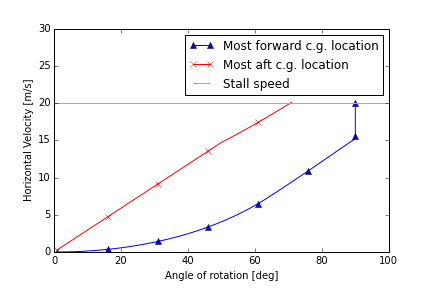
\includegraphics[width=0.6\textwidth]{StabilityandControl/Figures/transition.png}
    \caption{Graph of Angle of Rotation vs. Horizontal Velocity}
    \label{fig:tran_vert_to_hori}
\end{figure}

\section{Verification \& Validation}
\label{sec:veri_vali_snc}
In this section the verification and validation of the stability and control analysis and design is performed.

\paragraph{Tail Configuration}
The T-tail configuration choice can be validated by confirming that the downwash caused by the wing calculated using xflr5 is in the order of magnitude of 0.001. Since this was one of the main reasons the T-tail was chosen, it can be considered validated.

The incidence angle of the horizontal tailplane was checked by inspecting if the angle has a realistic value. Angles between -3 and 3 degrees are typically used \cite[67]{raymer}. Hence, the design value of 2.6 degrees lies within realistic boundaries.

\paragraph{Longitudinal Stability \& Control}
The c.g. position as a function of the leading edge calculated in the c.g. plot can be verified by calculating the actual c.g. position of the final CATIA model for the actual leading edge position and comparing it to the point on the curve. Due to time constraints, this was not possible but it can be considered as a future recommendation. The c.g. position is now verified by making hand calculations for the minimum and maximum c.g. range for a certain leading edge position and comparing it to the value in the python code. Another way the c.g. plot was verified was to check if special inputs (e.g. all masses zero, all arms zero, all arms in the middle) also gave the required, known output (e.g. error because of dividing by zero, c.g. is zero, c.g. is in the middle). Finally, a sanity check was performed on the final c.g. range. For example: checking whether the c.g. lies inside the fuselage.

The scissor plot can be validated by checking if all the assumptions used in the model for the stability and control curve are valid. In \autoref{sec:assu_snc}, all assumptions used are explained and the effects and deviations from reality are mentioned. As can be seen, the assumptions needed for the control and stability curve are only deviating slightly. The calculations are verified by checking if the input coefficients all have the correct sign and magnitude. For instance, the minimum tail lift coefficient should not exceed minus one, the lift slope coefficient should be positive and have a magnitude of one. The results of the scissor plot can be verified by performing a sanity check. Attention can be paid to the slope and the shift of the curves. For example, the neutral point should lie behind the leading edge, the slope of the control curve should be negative and the slope of the stability curve should be positive.

\paragraph{Lateral/Directional Stability \& Control}
The method used to size the vertical tailplane was validated by comparing the calculated surface area with that of the surface area estimated through the statistical method outlined in literature \cite[112]{raymer}. The method based on statistics makes use of typical vertical tail volume coefficients (c$_{vt}$) from which the surface area can by calculated as follows:

\begin{equation}
\label{eq:vert_tail_coef}
S_{vertical} = \frac{c_{vt} \cdot b_{w} \cdot S}{l_{v}}
\end{equation}

It is very difficult to find typical vertical tailplane volume coefficients for UAVs however using a typical value for light aircraft, a surface area in the same order of magnitude is obtained (S$_{vertical}$ of 0.04 m$^{2}$).

\paragraph{Control Surfaces}
In order to check the control surface results, the moment generated by the control surface was calculated by hand and checked with the required moment it is supposed to generate. Also, the code was checked by putting different values for deflection angles (e.g. delta = 0 deg, delta = 30 deg) in the code and verifying if the outputs are reasonable.

The maximum hinge moment produced by the control surfaces was verified by doing the calculation by hand for the maximum deflection angle and checking whether the values comply.

\paragraph{Vertical Flight Manoeuvres}
The required power splits were calculated using a python script. This script was validated by calculating the inverse, beginning with the outputs and seeing whether the inputs were obtained as results. The inputs of the main python script were also validated with had calculations to ensure that the script was executed using valid inputs. 

Another way the the script was validated was by setting the angular accelerations for pitch, roll and yaw ($\alpha{pitch}$, $\alpha{roll}$ \& $\alpha{yaw}$) to zero. This was done to ensure that the output of the code, given this condition, was simply the power split calculated for hovering.


%recommendations: investigate dynamic stability
    \chapter{Structural Analysis}
\setlength{\parindent}{15pt}
\label{ch:stru_anal}



%PLEASE ADHERE TO THIS STRUCTURE
%\section{Design Approach}

%\section{Assumption}

%\section{Analysis}

%\section{Verification \& Validation}

%\section{Results}

\section{Design Approach}
\label{sec:desi_stru}



\section{Assumptions}
\label{sec:assu_stru}

\begin{itemize}
    \item Stringers are only loaded in bending and axial stress.
    \item The fuselage frames are loaded purely in shear
    \item The fuselage skin carries only shear stresses
\end{itemize}

\section{Analysis}
\label{sec:anal_stru}

\begin{equation}
\label{eq:boom}
    B_{1} = \frac{t_{D}b}{6}\left ( 2+\frac{\sigma _{2}}{\sigma _{1}} \right )
\end{equation}

\section{Verification \& Validation}
\label{sec:veri_vali}
\section{Results}
\label{sec:resu_stru}
%%%%%%%%%%% THIS IS THE OLD PAYLOAD CHAPTER COMMENTED OUT FOR NOW %%%%%%%%%%
\begin{comment}
In this section, the fuselage and payload compartment design will be explained. First, the layout of the fuselage is presented. Based on this, a stress analysis is made. After that, different options for materials are compared. Finally, all design decisions, based on the previous analysis, are presented.


\section{Fuselage Layout}
\label{sec:fuse_layo}
Explain general layout of the fuselage, like where the torsion boxes, stringers etc will be located


\section{Stress Analysis}
\label{sec:stre_anal}




\section{Material Analysis}%Written by Steph
\label{sec:mate_anal}

In this section, an overview is given of different materials that could possibly be used to manufacture the UAV. Some relative qualities are presented for each material option. In \autoref{tab:mate_gene} all materials that contribute to the strength of the structure are given. In \autoref{tab:mate_clos} the possible materials for the payload bay closing system that do not contribute to the stress bearing capacities are compared. The cost is not discussed in these tables, since for the expected quantity of products, fibre reinforced composites can compete with steel\footnotemark.
\footnotetext{\url{http://msl1.mit.edu/MIB/3.57/LectNotes/gm_tech_composites.pdf}, Accessed 14-06-2017}



\begin{table}[h]
    \centering
    \caption{Overview of material options \cite{material}}
    \label{tab:mate_gene}
    \begin{tabularx}{\textwidth}{LCCC}
    \toprule
    \textbf{Skin} &  \textbf{Weight [g/$cm^3$] }  & \textbf{Thickness} & \textbf{Tensile strength}
    \\ \midrule
    Glass fibre composite    
    &  2.5 
    & 
    & 3.5 - 4.6 GPa\footnotemark
    \\ \hdashline
    Carbon fibre composite    & 1.8 & &
    \\ \hdashline
    Aluminium       & 2.7  & &
    \\ \hdashline
    Steel           & 7.9 & &
    \\ \hdashline
    Titanium        & 4.4 & &
    \\ \hdashline
    Kevlar          & 1.4 & &
    \\ \hdashline
    Wood            & 0.6 & &
    \\ \hdashline
    Plastic         & 1.2 & &
    \\ \hdashline
    Cloth           & & &
    \\ \bottomrule
    \end{tabularx}
\end{table}


\addtocounter{footnote}{2}
\stepcounter{footnote}\footnotetext{\url{https://www.researchgate.net/publication/265346634_Glass_fiber-reinforced_polymer_composites_-_A_review}, Accessed 14-06-2017} %flass fibre weight
\stepcounter{footnote}\footnotetext{\url{http://textilelearner.blogspot.nl/2012/09/glass-fiber-composites-properties-of.html}, Accessed 14-06-2017}%glass fibre strength


\section{Fuselage Design}


\subsection{Fuselage Closing}%Written by Steph
\label{sec:fuse_clos}
ADD EXPLANATION ABOUT DIFFERENCE BETWEEN DROPPABLE PAYLOAD AND PAYLOAD THAT IS KEPT ON BOARD AND THEREFORE LOADS CAN BE CARRIED


In this section, the closing mechanism of the payload bay is explained. In the midterm report, no intentions were expressed of incorporating such a system \cite{midterm}. However, since for some missions, (part of) the payload will be released from the fuselage, it needs to be possible to close the fuselage to prevent excessive drag. The possibility of closing the fuselage also allows for different payload shapes to be transported without extra packaging.


To determine how the system would look, first some brainstorming was done. Different options were swinging doors, sliding doors, a mechanism in which the door would be positioned above the payload, and a roller system. Each of these systems has advantages and disadvantages. In \autoref{tab:fuse_clos_comp}, some of these are listed. 

\begin{table}[h]
    \centering
    \caption{Comparison of different fuselage closing mechanisms}
    \label{tab:fuse_clos_comp}
    \begin{tabularx}{\textwidth}{>{\small}l L L}
    \toprule
    \textbf{System} & \textbf{Negatives} & \textbf{Positives}
    \\ \midrule
    Swinging doors & Difficult to transfer stresses, extra connecting mechanism is required. Heavy. Large. &  Closes automatically as payload is dropped.  
    \\ \hdashline
    Sliding doors & Difficult to transfer stresses, extra connecting mechanism is required. Heavy. Large. &  Closes automatically as payload is dropped.
    \\ \hdashline
    Fall-down door & Heavy. Large. & Can transfer stresses. Closes automatically as payload is dropped. 
    \\ \hdashline
    Roller system & Requires an additional rolling system. & Can include bars to transfer stresses. Light as it can be partially made out of fabric. Compact.
    \\ \bottomrule
    \end{tabularx}
\end{table}


It was decided that the most important aspect in the design of the closing was the ability to help the rest of the fuselage sustain stresses. This is because if the bottom of the fuselage can not transfer any stresses, the whole design needs to be a lot stronger. Because the roller system is expected to be the lightest and as it enables including bars that can take some stresses, this is the system that will be used for closing the fuselage.

\paragraph{System Layout}
The closing system will consist of 
\end{comment}
    \chapter{Command \& Data Handling}%Worked on by Chris+Steph
\setlength{\parindent}{15pt}
\label{ch:avio_grou_hand} %Dont change this label (we know it does not adhere to the style)

In this chapter, the command and data handling is designed. This includes all UAV avionics and the general design of the ground station. First, in \autoref{sec:desi_appr_comm}, the design approach is illustrated in a flow chart. Then, in \autoref{sec:avio_grou_stat}, the avionics of the UAV are designed and in \autoref{sec:grou_hand_payl} the ground station is explained together with different payload modules. Finally, sections \ref{sec:comm_flow_diag}, \ref{sec:data_hand_bloc_diag}, \ref{sec:hw_sw_bloc_diag} and \ref{sec:elec_bloc_diag} show the communication flow diagram, data handling block diagram, hardware diagram, software diagram and last the electrical block diagram.
 
\section{Design Approach}
\label{sec:desi_appr_comm}
In \autoref{fig:comm_data_work} the design approach is visualised. 

\begin{figure}[htb]
    \centering
    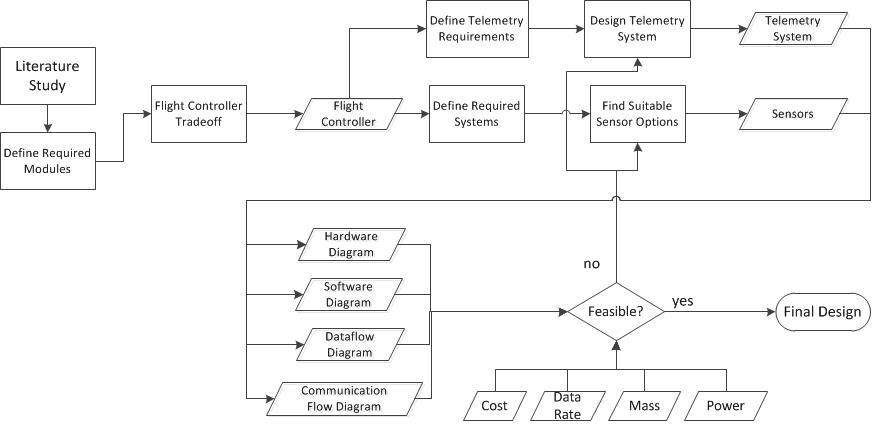
\includegraphics[width=\textwidth]{./CommandDataHandling/Figures/WorkFlow}
    \caption{Command and Data Handling Work Flow Diagram}
    \label{fig:comm_data_work}
\end{figure}



\section{Avionics}% and Ground Station}%Written by Steph, Chris + Steph responsible/worked on
\label{sec:avio_grou_stat}
In this section, all avionics used in the preliminary design will be explained. In order to cut down on cost as batch size increases, in future design stages some of the selected systems will be replaced by in-house designed systems. That would, however mean requirement SYS-OP-2.3 (that states the electrical components used should be off-the-shelf parts) has to be discarded.  

An overview of the systems that were selected can be found in \autoref{tab:avio_subs}. This was done based on the requirements in the SYS-OP category %(maybe refer to requirements)
and on extensive online research. Further specifications on the selected systems can also be found here. In \autoref{sec:avio_trad_off} a comparison is made between different available systems. The design of the telemetry system is discussed in \autoref{sec:tele_syst} and in \autoref{sec:grou_stat_layo} the layout of the ground station is explained. Then in \autoref{sec:encr} a secure communication protocol is established. 
\nomenclature[A]{GPS}{Global Positioning System}
\nomenclature[A]{BVLOS}{Beyond Visual Line of Sight}
%SUS-OP-2.3 the UAV shall be constructed with off-the-shelf electrical components use this for justifying pixhawk system
%&SYS-OP-2.5.3,4,5 Object avoidance, ground avoidance
%SYS-OP-2.7 Night conditions.......
%Include paparazzi STATE with software http://wiki.paparazziuav.org/wiki/Pixhawk
%Explain what is meant with modularity
%SYS-OP-2.9.2:The safe mode of the UAV shall have a return-to-base function.SYS-OP-2.9.3:autonomous emergency landing


\begin{table}[ht]
    \centering
    \caption{List of Avionics Subsystem Components}
    \label{tab:avio_subs}
    \begin{tabularx}{\textwidth}{>{\small}p{.15\textwidth} >{\small}p{.18\textwidth} >{\small}p{.12\textwidth} L}
    \toprule 
    \textbf{System type}     & \textbf{Selected system} & \textbf{Price} &\textbf{System specifications} 
    \\ \midrule
    Flight control module      & Pixhawk 2.1\footnotemark & USD 198,- & Isolated IMU (3x accelerometer, 3x gyroscope, 3x magnetometer, 2x barometer), flight controller board, multiple input ports, micro SD card for internal memory. Estimated size 10x5x2 cm, estimated weight 200 g. %this one goes last when all the others have been filled in
    \\ \hdashline
    Software            & Paparazzi\footnotemark & USD 0,- & Open-source, easy implementation of different functionalities
    \\ \hdashline
    Ground avoidance system & SF30-C Laser Rangefinder\footnotemark & USD 699,- & Range 100 m, accuracy $\pm$0.1 m, weight 35 g, dimensions 30 x 55 x 50 mm
    \\ \hdashline 
    Object avoidance system & Jenoptik DLEM 20\footnotemark & Estimated at EUR 1000,- & Sensor uses flight control module for avoidance of obstacles. Dimensions 50 mm x 22 mm x 34 mm, weight 33 g, range 5 km, accuracy 0.5 m.
    \\ \hdashline
    GPS & Here GNSS for Pixhawk\footnotemark & USD 48,- & Concurrent reception of up to three GNSS, -167 dBm navigation sensitivity, weight 49 g, dimensions 8x8x2 cm.
    \\ \hdashline
    2x Airdata sensors & Digital Airspeed sensor\footnotemark & USD 130 & 0.84 Pa resolution, Kit dimension 24x17x10 mm. Mounted at both wingtips. 
    \\ \hdashline
    Radio Control & Frsky V8FR-II receiver\footnotemark & EUR 14,- & 2.4 GHz, Weight 39g, dimensions 34x19x8 mm. \\
    & FrSky 2.4GHz Accst Taranis X9D PLUS\footnotemark & EUR 160,- & RC Transmitter for the ground station. 
    \\ \hdashline
    Telemetry & u-Blox TOBY L2-series \footnotemark &   EUR 60,- & Weight 4.8g, dimensions 25x36x3 mm.
    \\ \hdashline
    Payload link & USB or other cable & Estimated at EUR 10,- & Pixhawk module has multiple extra ports for both power and camera modules.
    \\ \midrule
     & Estimated total: & EUR 2200,- & Estimated total size: 400 cm$^3$, 400g.
    \\ \bottomrule
    \end{tabularx}
\end{table}


\addtocounter{footnote}{-9}
\stepcounter{footnote}\footnotetext{\url{http://www.robotshop.com/en/pixhawk-21-standard-set.html}, Accessed 12-06-2017}
\stepcounter{footnote}\footnotetext{\label{ft:pixhawk}\url{http://wiki.paparazziuav.org/wiki/Pixhawk}, Accessed 22-06-2017}
\stepcounter{footnote}\footnotetext{\url{http://www.robotshop.com/en/sf30-c-laser-rangefinder-100m.html}, Accessed 13-06-2017}
\stepcounter{footnote}\footnotetext{\url{https://www.jenoptik.com/products/defense-and-security/laser-rangefinders/oem-modules-system-integration/dlem}, Accessed 13-06-2017}
\stepcounter{footnote}\footnotetext{\url{http://store.jdrones.com/digital_airspeed_sensor_p/senair02kit.htm}, Accessed 21-06-2017}
\stepcounter{footnote}\footnotetext{\url{https://www.unmannedtechshop.co.uk/here-gnss-module-for-pixhawk-2/}, Accessed 22-06-2017}
\stepcounter{footnote}\footnotetext{\url{https://hobbyking.com/en_us/frsky-v8fr-ii-2-4ghz-8ch-receiver-hv.html}, Accessed 20-06-2017}
\stepcounter{footnote}\footnotetext{\url{https://hobbyking.com/en_us/frsky-2-4ghz-accst-taranis-x9d-plus-digital-telemetry-radio-system-mode-2.html}, Accessed 22-06-2017}
\stepcounter{footnote}\footnotetext{\url{https://www.u-blox.com/en/product/toby-l2-series}, Accessed 19-06-2017}

\begin{comment}
http://www.robotshop.com/en/uav-drone-sensors.html
http://pixhawk.org
http://www.robotshop.com/blog/en/how-to-make-a-drone-uav-lesson-4-flight-controller-15191
\end{comment}


\subsection{Trade-off}
\label{sec:avio_trad_off}
In this section, different options for the flight control and positioning systems are discussed. The systems need to be able to measure axial and angular accelerations, orientation, attitude, altitude, distance to the ground, distance to obstacles and determine its global position. The communication system will be discussed in \autoref{sec:tele_syst}.


In \autoref{tab:flig_cont}, an overview of (combinations of) systems is given that can determine all previously mentioned aspects and are able to process some data from for example monitoring equipment. For some of the systems the exact size or weight is not known. In these cases, sizes are either estimated based on reviews an images or not given when this was deemed too inaccurate. %FOOTNOTE EXPLAIN TRADE OFF TABLE AND OUTCOME EXPLAIN CHOICE OF GROUND AVOIDANCE SYSTEM AND OBJECT AVOIDANCE SYSTEM
This overview is then used to perform a trade-off between the different system layouts. First, weights were determined. The CPU has been assigned with the greatest weight factor, since it is the driving factor in a lot of missions. Size (weight and dimensions), modularity (the amount of available connections) and accuracy have been given equal weights. They are considered very important, however not as significant as the CPU. Size can make it very hard to carry the module and could pose some severe constraints on the structure, modularity is essential to the connection of different controllers and monitors yet in most boards, it is possible to overcome this by installing intermediate connectors, and accuracy is essential to the control of the UAV. Then cost, GPS and software were assigned with the smallest weight. The cost of all of the systems was found to be within the budget limits, a separate GPS system could be added in case the current system is not accurate enough, and software modules could also be changed. Then each of the concepts has been graded per criterion, where `- -' means that performance is extremely poor, `0' means average and `+ +' means very beneficial to the design or system. Then based on these weights and scores, the systems have been assigned with a grade that was found by adding or subtracting the weight factors as the scores stated it, then dividing by two and adding 40. That means scores between -15 and 105 are theoretically possible, yet all scores are between 0 and 100. The range was made larger (than from 0 to 100) to make different scores more outspoken.




\begin{table}[ht]
    \centering
    \caption{Overview of Flight Control Systems}
    \label{tab:flig_cont}
    \begin{tabularx}{\textwidth}{>{\small}p{.12\linewidth} L  >{\small}p{.13\textwidth}  }
    \toprule
\textbf{System(s) }     & \textbf{Specifications }       &\textbf{Price, Size}                                %& \textbf{Positives, Negatives}                                                                                        
\\ \midrule
Navio2 Autopilot, Raspberry Pi 3                       & GNSS receiver, extension ports, includes power module, dual IMU, 10 cm resolution barometer, 14 PWM servo outputs, 1.2GHz 64-bit quad-core ARM Cortex-A53 CPU, Integrated 802.11n wireless LAN and Bluetooth 4.1, software still required.                                                                                                                                                                                                                                                                                  & USD253,   2x   55x65x15 mm, 68g                                  % & Provides all desired ports for extra equipment, processor is strong enough. Software still needs to be designed.                                                             
\\ \hdashline             
Radiolink PixHawk 1             & 32bit STM32F427 Cortex M4 corewith FPU, 256KB RAM, 3-axis IMU, 16 bit gyroscope, 14 bit accelerometer and magnetometer. Size estimated.                         & USD140, 100x40x20 mm, 100g                                     %& GPS already included, relatively cheap. Possibly requires extra ports. Also IMUs processing capacity could be better. Software available 
\\ \hdashline
Lynxmotion Quadrino     & Nano Drone/UAV Flight Controller, Software included, IMU, Explansion ports, ATmega 2560 (256Kb flash @ 16MHz) Processor.                                                                 & USD150, 53x53x17 mm                                                                                                                           %& Software included.  Meant for smaller category drones, processor might not be able to handle it.    GPS included                                                                  
\\ \hdashline 
MWC MultiWii  & 2 Servo output for camera (only available when using 4 motors or less), Separate 3.3V and 5V LDO voltage regulators.                                                                                                                                                                                                                                                & USD23,      36x36x2 mm                                                                                                               %& Small, cheap.  Output/input port and processing capacity too small, arduino required..                                                                                              
\\ \hdashline
AfroFlight Naze32 Rev6                   & Up to 8 ch RC input, 32-bit processor running at 3.3V/72MHz. BMP280 barometer.                                                                                                & USD21,      36x36 mm,                                                                             7.3g  %& Small, cheap. Meant for quadcopter racing -- not suitable for a lot of data processing.                                                             
\\ \hdashline
DJI Naza-M V2                        & Software included,  Intelligent Orientation Control, PPM, S-BUS \& Ordinary Receiver Supported, Built-in Gimbal Stabilisation Function, Remote Gain Adjustment, Hovering Accuracy (GPS Mode) Vertical:$\pm$0.8m, Horizontal:$\pm$2.5m .                                               & USD 159,   4x  45x45x10 mm, 95 g             
                %& Software available, function extensions possible, GPS included. Not very accurate, not certain if CPU can handle all camera data. Relatively large.                              
\\ \hdashline 
Pixhawk 2.1, Here+ GNSS                    & Modular design for flexibility, Triple Redundant IMU system, Modular cube. All inputs/outputs in one single DF17 connector, Concurrent reception of up to three GNSS, -167 dBm navigation sensitivity.                                                                                                                                        & USD246, GPS 79x82x17 mm, 49g 
% & Has a lot of modular options which is ideal for the different payload modules. Also has good processing memory and availability to put in an external memory card.  Relatively large, however would still fit in the design.   
\\ \hdashline
Paparazzi           & Open source software and hardware, all required components can be installed, manuals available.    Hardware cost and size estimated.         &USD100, 50x50x10 mm, 50g
\\ \bottomrule
    \end{tabularx}
\end{table}











\begin{table}[ht]
    \setlength\extrarowheight{5pt}
    \setlength\arrayrulewidth{1pt}
    \centering
    \caption{Flight Control Trade-Off}
    \label{tab:avio_trad_off}
    \begin{tabular}{r|
    |>{\centering}p{1cm}
    |>{\centering}p{.5cm}
    |>{\centering}p{2cm}
    |>{\centering}p{1cm}
    |>{\centering}p{.5cm}
    |>{\centering}p{1cm}
    |>{\centering}p{.5cm}
    | c } 
    \raggedright \textbf{Concept \rotatebox{90}{\hspace{0.5cm}Criterion}}        & 
    \rotatebox{90}{\textbf{Size}}                            &
    \rotatebox{90}{\textbf{Cost}}                                   & 
    \rotatebox{90}{\textbf{CPU}}                            & 
    \rotatebox{90}{\textbf{Modularity}}                        & 
    \rotatebox{90}{\textbf{GPS}}                       &
    \rotatebox{90}{\textbf{Accuracy}}                         &
    \rotatebox{90}{\textbf{Software}}       &
    \rotatebox{90}{\textbf{Result}}
    \\\hline
    Navio2      &
    \cellcolor[HTML]{FFC000}-    &
    \cellcolor[HTML]{FFC000}-    &
    \cellcolor[HTML]{00B050}++   &
    \cellcolor[HTML]{00B050}++   &
    \cellcolor[HTML]{92D050}+    &
    \cellcolor[HTML]{92D050}+    &
    \cellcolor[HTML]{FFC000}-    &
    \cellcolor[HTML]{92D050}\textbf{78}
    \\[5pt]\hline
    Pixhawk 1          &
    \cellcolor[HTML]{FFFF00}0    &
    \cellcolor[HTML]{FFFF00}0    &
    \cellcolor[HTML]{92D050}+    &
    \cellcolor[HTML]{00B050}++   &
    \cellcolor[HTML]{92D050}+    &
    \cellcolor[HTML]{92D050}+    &
    \cellcolor[HTML]{92D050}+    &
    \cellcolor[HTML]{92D050}\textbf{70}
    \\[5pt]\hline
    Lynxmotion      &
    \cellcolor[HTML]{92D050}+    &
    \cellcolor[HTML]{FFFF00}0    &
    \cellcolor[HTML]{FFFF00}0    &
    \cellcolor[HTML]{92D050}+    &
    \cellcolor[HTML]{92D050}+    &
    \cellcolor[HTML]{00B050}++   &
    \cellcolor[HTML]{92D050}+    &
    \cellcolor[HTML]{FFFF00}\textbf{65}
    \\[5pt]\hline
    MultiWii       &
    \cellcolor[HTML]{00B050}++   &
    \cellcolor[HTML]{00B050}++   &
    \cellcolor[HTML]{FF0000}- -   &
    \cellcolor[HTML]{FF0000}- -   &
    \cellcolor[HTML]{FFC000}-    &
    \cellcolor[HTML]{FFFF00}0    &
    \cellcolor[HTML]{00B050}++   &
    \cellcolor[HTML]{FF0000}\textbf{28}
    \\[5pt]\hline
    Afroflight   &
    \cellcolor[HTML]{00B050}++   &
    \cellcolor[HTML]{00B050}++   &
    \cellcolor[HTML]{FF0000}- -   &
    \cellcolor[HTML]{FFC000}-    &
    \cellcolor[HTML]{FFC000}-    &
    \cellcolor[HTML]{FFFF00}0    &
    \cellcolor[HTML]{FFC000}-    &
    \cellcolor[HTML]{FF0000}\textbf{25} 
    \\[5pt]\hline
    DJI Naza M   &
    \cellcolor[HTML]{FF0000}- -   &
    \cellcolor[HTML]{FFFF00}0    &
    \cellcolor[HTML]{92D050}+    &
    \cellcolor[HTML]{92D050}+    &
    \cellcolor[HTML]{00B050}++   &
    \cellcolor[HTML]{FF0000}- -   &
    \cellcolor[HTML]{92D050}+    &
    \cellcolor[HTML]{FFC000}\textbf{43} 
    \\[5pt]\hline
    Pixhawk 2.1   &
    \cellcolor[HTML]{FFFF00}0    &
    \cellcolor[HTML]{FFC000}-    &
    \cellcolor[HTML]{00B050}++   &
    \cellcolor[HTML]{00B050}++   &
    \cellcolor[HTML]{00B050}++   &
    \cellcolor[HTML]{92D050}+    &
    \cellcolor[HTML]{92D050}+    &
    \cellcolor[HTML]{00B050}\textbf{80} 
    \\[5pt]\hline 
    Paparazzi &
    \cellcolor[HTML]{92D050}+   &
    \cellcolor[HTML]{FFFF00}0   &
    \cellcolor[HTML]{00B050}++  &
    \cellcolor[HTML]{00B050}++  &
    \cellcolor[HTML]{00B050}++  &
    \cellcolor[HTML]{00B050}++  &
    \cellcolor[HTML]{00B050}++  &
    \cellcolor[HTML]{00B050}\textbf{95}  
    \\[5pt] \hline\hline
    Weight          &
    10              &
    5              &
    20              &
    10              &
    5              &
    10              &
    5           &
    \\[5pt]
    \end{tabular}
\end{table}









From \autoref{tab:avio_trad_off} it can be seen that the MultiWii and Afroflight system are not suitable for this UAV. The DJI Naza M also underperforms, however, not as much as the other two. On the other hand, the Pixhawk 2.1 and the Paparazzi system are the winnners of this trade-off, closely followed by the Navio2 system. Solely based on the trade-off, the most logical option to choose the Paparazzi system. However, this system also has open-source hardware, which means it still needs to be built. Requirement SYS-OP-2.3 states, however, that all electrical components should be off-the-shelf. The Paparazzi system is not qualified as such, and therefore, the hardware used will be the Pixhawk 2.1. Since the Paparazzi software does allow for easy adaption as it is open-source, this will be used instead of the Pixhawk software. Paparazzi software is easily implemented on the Pixhawk module\footnote{See footnote \ref{ft:pixhawk}.}.




%It was decided to use a ready-to-use flight control system, instead of installing the different components separately. Therefore, the system needs to consist at least  of an inertia measurement unit (IMU) or accelerometer plus gyroscope to determine accelerations, a compass or magnetometer to determine orientation, a pressure meter and a system that measures the distance to the ground, and preferably a Global Positioning System (GPS). In order to decrease the chance of burnout, a power brick is included in the Pixhawk module to transform the battery voltage to the flight controller voltage and to monitor the battery properties. For object avoidance, two laser sensors will be installed. One with a short range for ground detection, and one able to scan objects that are very far away, for collision avoidance.






\paragraph{Object Avoidance} The object avoidance system was selected after the flight control module. Initially, a trade-off would be performed on these as well. Both a ground sensor as well as a sensor that functions as the `eyes' of the UAV needed to be selected. For these sensors, different options are available. Some options and their (dis)advantages can be seen in \autoref{tab:obje_avoi}. Based on this comparison and the need for a sensor that can detect objects located up to 3 km away (Requirement SUB-AV-3.2), laser rangefinders were found to be the most suitable option. Some research was done on suitable laser rangefinders, and it was found that especially for the object avoidance, not a lot of options were present. The selected ground detection system was the cheapest one within  acceptable sizes and acceptable detection range (Requirement SUB-AV-3.3), while the selected object detection system was the only one that was within acceptable size limits while being able to detect objects very far away (Requirement SUB-AV-3.2). The specifications on these systems can be found in \autoref{tab:avio_subs}.



\begin{table}
    \centering
    \caption{Object Avoidance Sensor Types\protect\footnotemark }
    \label{tab:obje_avoi}
    \begin{tabularx}{\textwidth}{>{\small}p{.11\textwidth} >{\small}p{.4\textwidth} L}
    \toprule \bfseries
    Type        & \bfseries Advantages            & \bfseries Disadvantages
    \\ \midrule
    Laser rangefinder     
    & Ranges varying from 10 cm to up to 25 km. Laser has to return, yet does this at the speed of light making it very fast.
    & Accuracy comes at high cost. Eye-safety must be taken into account meaning not all lasers can be used (only class 1 and 2)\footnotemark
    \\ \hdashline
    LIDAR       
    & Very accurate.
    & Complete 3D surfaces can be mapped, which means more CPU is used than required for the purpose, expensive, large, heavy.
    \\ \hdashline
    Infrared
    & Cheap, direct response, can also be used at night.
    & Very sensitive to sunlight.
    \\ \hdashline
    Doppler radar
    & Used more often in aviation.
    & Measures relative velocity, not distance; signal needs to bounce back.
    \\ \hdashline
    SONAR
    & Can also detect very small objects.
    & Very expensive, large.
    \\ \bottomrule
    \end{tabularx}
\end{table}





\addtocounter{footnote}{-2}
\stepcounter{footnote}\footnotetext{\url{https://www.intorobotics.com/types-sensors-target-detection-tracking/}, Accessed 20-06-2017}
\stepcounter{footnote}\footnotetext{\url{https://www.rli.com/resources/articles/classification.aspx}, Accessed 20-06-2017}



\subsection{Telemetry System}%Made by Chris
\label{sec:tele_syst}

In this section, the Radio Control, (RC), system used for Visual Line of Sight, (VLOS), is discussed. Then, different possible telemetry systems for BVLOS communication are introduced and a final system is chosen.

\nomenclature[A]{VLOS}{Visual Line of Sight}

\paragraph{VLOS}

In order to control the drone in VLOS, a RC receiver is added to the telemetry system of the drone. The main purpose of this receiver is to obtain flight commands send by the operator while in VLOS. These flight commands are send directly to the UAV and are used in order to change thrust and provide control over the different control surfaces. This means, the operator can control the deflection angles and mangitude of thrust directly via the controller. 

Although the long range telemetry system in the next section could also be used for this purpose, a RC sender is preferred in close range due to the lower latency (as a direct link is established between operator and drone). Also the reliability of an RC link is higher, as the codes are not modulated and package loss is decreased due to the closer range.     

One disadvantage of the RC link is the fact that it is only used as a one-way link. Measurements of the different sensors are not send towards the ground station and hence it is only used for VLOS control. Data gathered on-board the UAV is send using the cellular link or has to be stored on the internal memory in case the cellular link breaks or is not available.

The most common RC link uses a 2.4 GHz frequency. Comparing different 2.4 GHz receivers, it was concluded, that a Frsky V8FR-II receiver will be used\footnote{\url{https://hobbyking.com/en_us/frsky-v8fr-ii-2-4ghz-8ch-receiver-hv.html}, Accessed 19-06-2017}. It uses eight channels, four used to simultaneously control rudder (change in yaw angle), elevator (change in pitch angle), throttle (change in thrust) and ailerons (change in roll angle). One remaining channel is then used for the tilting mechanisms of the engines, making it possible to manually transition from vertical to horizontal flight. The last three channels can be used for different payload modules which might require some kind of control, this can included opening and closing of the payload bay, rotating of cameras or dropping of payload. In case none of these are necessary, it can be decided that the three remaining channels are coupled to the 4 engine tilting mechanisms separately. This makes it possible to control the rotation of a single engine and can be used for control in vertical flight for example.



\paragraph{BVLOS}

The main requirement set for the BVLOS telemetry system is given by requirement SYS-PF-1.3, stating that the UAV, shall be capable of achieving a range of 200 km. As radio frequency communication can not reach these ranges, 2 alternatives are presented in this section: 
\nomenclature[A]{RC}{Radio Control}




\begin{enumerate}
\item{\textbf{Satellite Modem}}

In order to increase the range, a satellite modem could be used. This first sends the data towards a satellite which in turn redirects it towards the drone. The main advantage is that most areas of the Earth are covered and BVLOS operation is thus possible. Using a satellite modem, there are no range limitation. Major disadvantage is the  higher latency, as propagation and processing delays can be up to one second for a geostationary satellite connection. Furthermore, costs for using a satellite link are expensive and data rate dependant. Comparing only the dataflow of the sensors, a constant flow of up to 65 kbps can be necessary (see \autoref{sec:data_hand_bloc_diag}). Using the Iridium satellite network, this results in a cost of around 6 euro per second transmitting all the relevant data, which does not include yet live video feeds or other data consuming devices mounted in the payload.\footnote{\url{http://www.rock7mobile.com/products-rockblock}, Accessed 19-6-2017}

\item{\textbf{GSM/LTE Modem}}

Global System for Mobile Communications (GSM) and Long Term Evolution (LTE) modems make use of mobile cellular networks for the data transfer. As mobile telecommunications are widely available nowadays, using a GSM/LTE modem greatly increases the range compared to a radio modem. On top of that, data rates of up to 50 Mbps can be achieved in good conditions.\footnote{\url{https://www.u-blox.com/sites/default/files/TOBY-L2_DataSheet_\%28UBX-13004573\%29.pdf}, Accessed 12-6-2017} Although this makes it possible to use BVLOS operation, cellular networks are less developed in poorer countries and do not cover the oceans at all. This reduces the possible operational area significantly compared to satellite networks. The cost of data services is relatively low compared to satellite links. Several distributors in the Netherlands provide 10 GB of data transfer for around EUR 30,- per month.\footnote{\url{https://www.kpn.com/mobiel/mobiel-internet/simkaart/mobiel-internet-standaard/1-jaar}, Accessed 19-6-2017} 
\end{enumerate}
\nomenclature[A]{GSM}{Global System for Mobile Communications}
\nomenclature[A]{LTE}{Long Term Evolution}
Although the higher coverage of satellite communication is preferred for save and rescue missions, the cost is limited and high data transfer is required in order to obtain a reliable video feed for monitoring. Furthermore, satellite communications require bigger antennas in order to achieve a safe and reliable data connection. Another major advantage of using cellular networks is the fact that the packages are send using conventional networking technologies and hence also routed this way. This makes it easier to securely deliver the messages, which is in more detail explained in Section \ref{sec:encr}. For these reasons, a GSM/LTE modem is used as larger range telemetry system. This then also comes with the advantage that in order to control and monitor the drone only an internet connection is necessary.

The chosen GSM/LTE modem is a u-Blox TOBY L2-series LTE Modem. It can be connected directly to the Pixhawk Flight Controller via UART. Care should be taken that the correct module is chosen depending on the geographical location where the drone is operating. 

\paragraph{Final Layout}

Finally, the UAV uses a cellular network connection as main telemetry system. Via an internet connected device, waypoints can be send to the telemetry module for navigation. The flight controller then chooses the best control inputs to perform the mission. Furthermore, higher data rates are supported using this connection, hence also attitude data and monitoring data is send on this channel.

A second, more reliable link is created using the RC connection. This connection can only be used for lower ranges (up to 2 km) and hence it is only used for VLOS. Using the RC channel, the operator can control the thrust as well as pitch, yaw and roll angles. Transitioning from vertical to horizontal flight will also be possible using the controller. RC communication is thus preferred in case a higher precision is required, as position determination is dependant on GPS accuracy. 

In case the flight controller receives messages from both links, the newest messages are preferred and performed. Furthermore, in case the main cellular link breaks, the flight controller tries to establish a connection with the RC transmitter. If no link is available within 10 seconds, a return to take-off procedure is performed during which the UAV aborts its mission and returns to its starting point. 






\subsection{Encryption}%Made by Chris
\label{sec:encr}

The UAV market is increasing significantly without a major consideration in the safety of the exchanged messages. This comes with the problem that an adversary can without major troubles control the drone. 

A secure communication should be confidential (only the receiver can read the message), authenticated (the receiver is sure who sent the message) and integer (nobody can change the message). However for the flight control communications of the drone it is of no relevance whether an adversary knows that the drone is going to perform a certain action, this section only focuses on authentication and integrity. In case data has to be confidential, it is recommended to look into different encryption techniques using less processing power. 

The protocol used for flight control message exchange is the Micro Air Vehicle Communication (MAVLink) protocol. It is used for internal communication between the different sensors and the flight controller as well as to transmit useful information as attitude, speed and battery status of the vehicle and to send new waypoints for control of the drone. Although the integrity of the messages is already ensured by the checksum, it only has a length of 2 bytes (16 bits). This checksum can be guessed easily by current computers and hence the scheme is not secure.
\nomenclature[A]{MAVLink}{Micro Air Vehicle Communication}
Integrity and authentication are obtained using a Message Authentication Code (MAC). Before the MAVLink data is send to the cellular network, a Hash-based message authentication code (HMAC) is attached to it. In order to prevent replay attacks, the current time and date will also be added to the message before calculating the MAC. The HMAC uses the same principles as the checksum explained before, however, it can only be calculated knowing a symmetric key, stored at both the internal memory of the ground station and the drone.  Furthermore, the length of the checksum is equal to 16 bits, a HMAC however can have a length of 128 bits, making it more secure. This scheme is only secure if no third party is able to access either the drone or the ground station. Regular exchange of the key improves the security of the system.
\nomenclature[A]{MAC}{Message Authentication Code}
\nomenclature[A]{HMAC}{Hash-based Message Authentication Code}


The preceding encryption algorithm makes sure that the drone does not accept any commands send by an unauthenticated device. Furthermore random noise errors and messages that have been interfered with are also discarded. The final message send over the cellular network is depicted in \autoref{fig:encr_mess}. Due to the fact that the cellular network is used to transmit the message, an IP header is added in front of the MAVLink message, which includes beside others routing information. It can size from 20-60 bytes depending on the optional fields. The MAC is added at the end of the message and is calculated using only the orange fields, the MAVLink Frame and the Time and Date (T/D).

\begin{figure}[htb]
    \centering
    
\includegraphics[width=\textwidth]{./CommandDataHandling/Figures/encryption}
    \caption{Final Message Layout}
    \label{fig:encr_mess}
\end{figure}






\section{Ground Handling and Payload}%made by Steph
\label{sec:grou_hand_payl}

In this section, some relevant aspects related to the ground handling are discussed: the payload mounting mechanism and the possible payload modules, as well the ground station layout.


\subsection{Ground Station Layout}%made by Steph
\label{sec:grou_stat_layo}
%what kind of data is shown on the ground station? And what functionalities are required? Without defining these, you can't justify any choice of hardware/software.



In this section, the different options for the ground station are discussed, after which a layout for the system is chosen. %maybe mention requirements
Before selecting a layout, the functionalities of the ground station are defined. This is done based on different aspects of the UAV missions.
\begin{description}
    \item[Automated flight control] The location of the UAV shall be displayed, as well as its velocity, heading and altitude. It shall also be possible to see the flight plan. Besides that, waypoints can be added and the destination can be changed. The battery percentage shall also be shown.  
    \item[Manual fligth control] Since the UAV is in VLOS, showing its location is redundant here. However, battery, attitude, heading and velocity are useful parameters and shall therefore be shown. It shall be possible to give directional inputs, that cause accelerations. 
    \item[Mission specific capacities] When a camera module is present in the payload, the recorded shall be visible on the ground station. The payload status shall also be visible, so whether a payload is present or not. In the case of a disposable payload, the payload bay closing mechanism must be operated. Therefore, in that case the status of the mechanism shall be shown, and it shall be possible to open or close it from the ground station.
\end{description}




The two categories to choose between are a large ground station with a case, displays and controls, or just software that can be installed on any tablet or laptop with an internet connection. It was decided that using software is preferred, since it allows for more flexibility in interfaces, which is beneficial for the variation of mission types. Also, a tablet is easier to transport. Furthermore, as cellular technology is used for communication, only an internet connection is required for control. The only disadvantage is that the UAV will have to rely more on the autopilot, because the inputs given on a tablet will not be control inputs, but waypoints. After some research on world network coverage, it was decided that using just software and a tablet is a viable option\footnotemark. However, to have manual control in VLOS, a RC controller is used. This will be incorporated in the system.
\footnotetext{\url{http://data.worldbank.org/indicator/IT.CEL.SETS.P2?view=map}, Accessed 12-06-2017}



It was decided to choose a system that is compatible with the Pixhawk system that was selected in \autoref{sec:avio_grou_stat}. Therefore,  Paparazzi software will be used\footnotemark. It is compatible with the Pixhawk, all sensors and equipment connected to it can be incorporated in the program because of the open-source character of the software.

\footnotetext{See \autoref{ft:pixhawk}.}

Then, in order to use the more reliable RC Link, as explained in \autoref{sec:tele_syst}, an RC transmitter is needed. A FrSky ACCST TARANIS X9D PLUS Digital Telemetry Radio System\footnotemark  is used for this, since it is recommended to use with the Pixhawk module and its pricing fits within the avionics and ground station budget. It supports at least the 8 channels available by the RC receiver and can hence be used for direct control of the aircraft.

\footnotetext{\url{https://hobbyking.com/en_us/frsky-2-4ghz-accst-taranis-x9d-plus-digital-telemetry-radio-system-mode-2.html}, Accessed 19-06-2017}



\subsection{Payload Mounting}

In this section, the payload mounting mechanism will be explained. For the closing mechanism of the fuselage, please refer to \autoref{sec:payl_bay_clos_syst}.


Since some missions require a droppable payload module, the mounting mechanism should allow for this. There also are cases in which it would be beneficial to only drop part of the payload, making it possible to take extra batteries or camera equipment. This means two things:

\begin{description}
\item[Modular payload] In order to enable for part of the payload to be dropped, it is possible to put in different pieces of payload, as long as they fit in 15x15 cm with varying lengths, and the total length of the payload modules does not exceed 1 m. In order to keep fragile payloads from shaking, magnets will be used.  
\item[Releasable payload] The payload will be mounted using a clipping system. Each module will have rigid bars, disposable ropes or something else that allows the module to be held. This is then clipped to a system that works similar to nippers. The `nippers' are mounted to two parallel bars, like in \autoref{fig:payl_moun_syst}.(3), and can be operated individually by the CPU. 
\end{description}

\begin{figure}
    \centering
    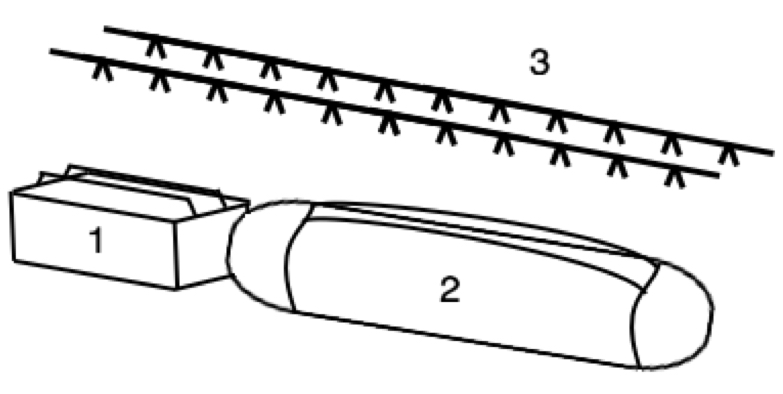
\includegraphics[width = .5\textwidth]{CommandDataHandling/Figures/Payload_module}
    \caption{Schematic Example of Payload Mounting System}
    \label{fig:payl_moun_syst}
\end{figure}







\subsection{Payload Bay Closing System}
\label{sec:payl_bay_clos_syst}
In this section, the closing mechanism of the payload bay is explained. In the midterm report, no intentions were expressed of incorporating such a system \cite{midterm}. However, since for some missions, (part of) the payload will be released from the fuselage, it needs to be possible to close the fuselage to prevent excessive drag. The possibility of closing the fuselage also allows for different payload shapes to be transported without extra packaging.


To determine how the system would look, first some brainstorming was done. Different options were swinging doors, sliding doors, a mechanism in which the door would be positioned above the payload, and a roller system. Each of these systems has advantages and disadvantages. In \autoref{tab:fuse_clos_comp}, some of these are listed. 

\begin{table}[ht]
    \centering
    \caption{Comparison of Different Fuselage Closing Mechanisms}
    \label{tab:fuse_clos_comp}
    \begin{tabularx}{\textwidth}{>{\small}l L L}
    \toprule
    \textbf{System} & \textbf{Negatives} & \textbf{Positives}
    \\ \midrule
    Swinging doors & Difficult to transfer stresses, extra connecting mechanism is required. Heavy. Large. &  Closes automatically as payload is dropped.  
    \\ \hdashline
    Sliding doors & Difficult to transfer stresses, extra connecting mechanism is required. Heavy. Large. &  Closes automatically as payload is dropped.
    \\ \hdashline
    Fall-down door & Heavy. Large. & Can transfer stresses. Closes automatically as payload is dropped. 
    \\ \hdashline
    Roller system & Requires an additional rolling system. & Can include bars to transfer stresses. Light as it can be partially made out of fabric. Compact.
    \\ \hdashline
    Discard entire module & Very unsustainable. Only closes the fuselage before release; this is actually not a closing mechanism. & Can transfer and sustain stresses considerably better than the other systems. 
    \\ \bottomrule
    \end{tabularx}
\end{table}


It was decided that the most important aspect in the design of the closing was the ability to help the rest of the fuselage sustain stresses. This is because if the bottom of the fuselage can not transfer any stresses, the whole design needs to be a lot stronger. Based on this, the decision was made to make a distinction between constant and in-flight removed payload.

\begin{description}
    \item[Constant payload] This is a payload module that is not dropped. Because a compete payload module can sustain a lot more stresses than a separate closing mechanism, as the walls of such a module also carry loads, in the missions that not require dropping the payload a closed box is used, like in \autoref{fig:payl_moun_syst}.(1).
    \item[Droppable payload] In the case of a payload that needs to be delivered in-flight, a separate small payload module is installed that closes the fuselage after payload release. This module will be installed next to the payload that is dropped, so that it only covers that part of the fuselage that needs to be closed. It will consist of a small box with dimensions 15x15 cm times the diameter of the rolled-up closing sheet. This shall be a roller system which consists of fabric to reduce the drag and bars to carry strength. Within the closing module, a small motor is present that operates the unwinding of the sheet. The module shall be connected to the CPU so that it closes the fuselage right after the payload is dropped.
\end{description}








\subsection{Payload Modules}
In this section, a short discussion on suggested payload modules for the different mission profiles will be given. The payload modules \textit{will not} be designed into full detail; however, components such as cameras are preferably chosen such that they are easily compatible with the Pixhawk flight control system. A modular clicking system will be installed, so that it is possible to drop (part of) the payload.

\begin{enumerate}
\item	\textbf{Search and rescue and support to disaster relief operations.} This requires a module that is able to locate the person(s) in need, and drop a help module. The difficulty in this module is that it will be dropped, so if an extra camera or battery is needed, those should be put in a separate module. As the object avoidance system that was chosen in \autoref{tab:avio_subs} only shows presence without being specific, some camera should be taken or dropping location would be based on GPS. The payload then only contains of a care package or buoy. Velocity and range are most important here, but a mission specific trade-off should be made between that performance and payload capacity.
\item	\textbf{Precision agriculture by monitoring of cattle and crops.} For this type of mission, high-quality camera equipment is required. Endurance is the most important feature for this mission type, so an extra battery will also be installed. A camera that takes images at a high frequency should be selected, so it is possible to still generate lift using the wings.
\item \textbf{Transportation of parcels at sea and on land.} This type of mission requires large range. Therefore it will probably make use of a separate battery payload module and parcel module, where maximum battery size is dependent on payload size.
\item \textbf{Inspection of extensive industrial assets and infrastructures such as railways, high-tension powerlines, pipelines, wind farms, etc.} This type of mission requires similar equipment as mission 2. The difference is that this mission type documents long-range objects, while the agricultural one should cover large areas. Therefore, range is very important in this mission type. It will also make use of high-quality camera equipment and if possible and extra battery module.
\item 	\textbf{Transportation of organs for transplants.} In the case of transporting organs, high velocity is very important. The payload should be well-protected, which means it will probably be light, yet large. Some room might be available for extra batteries. The payload will not be dropped, but the UAV will land for unloading, so a cooling case could be designed for this means.
\end{enumerate}


\section{Communication Flow Diagram}
\label{sec:comm_flow_diag}

In this section, the communication flow diagram is illustrated in \autoref{fig:comm_flow_diag}. It illustrates the flow to and from the UAV system to the environment. 

\begin{figure}[ht]
    \centering
    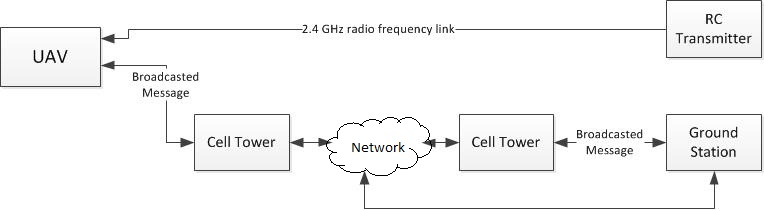
\includegraphics[width=.8\textwidth]{./CommandDataHandling/Figures/CommFlowDiagram.jpg}
    \caption{Communication Flow Block Diagram}
    \label{fig:comm_flow_diag}
\end{figure}

As explained in \autoref{sec:tele_syst}, the telemetry system consists of two different links, a direct link between the UAV and the control station using radio frequency and an indirect link using cellular technology. The radio frequency link is a one-way link to only send control commands to the flight controller. These commands are send using Pulse Width Modulation (PWM) techniques. As seen in \autoref{fig:comm_flow_diag}, data send using the mobile network is first broadcasted through the air until it reaches a cell tower. Using the routing information on the IP packet, the data is either routed directly towards the ground station (in case it is connected to the internet) or to the closest cell tower from the ground station (in case it is connected via the mobile network). In the latter case, the cell tower broadcasts the message and the ground station can receive it. The data send via the mobile network range from monitoring data to new waypoint or commands send to the drone to change its flight path. 

\nomenclature[A]{PWM}{Pulse Width Modulation}

\section{Data Handling Block Diagram}
\label{sec:data_hand_bloc_diag}

In this section, the data handling block diagram is depicted in \autoref{fig:data_hand_bloc_diag}. The main purpose of this diagram is to illustrate the different data flows across the system. Furthermore it depicts the sample rates and processing speeds. 

\begin{figure}[ht]
    \centering
    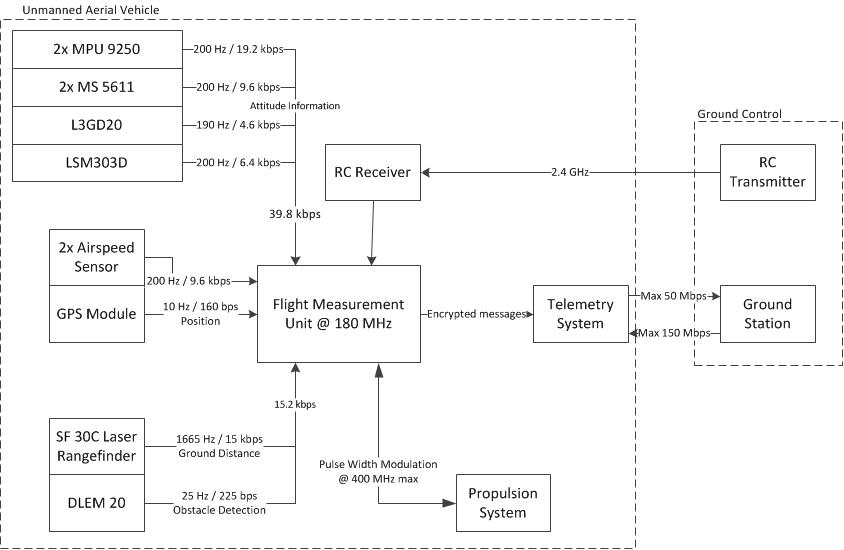
\includegraphics[width=0.8\textwidth]{./CommandDataHandling/Figures/DataDiagram.jpg}
    \caption{Data Handling Block Diagram}
    \label{fig:data_hand_bloc_diag}
\end{figure}

The attitude sensors can sample the information at different rates, however more sampling results in a bigger data flow and higher required processing power. It was assumed that sampling attitude information at a speed of 200 Hz results in a good overview of the UAV attitude. The sampling rates for the object avoidance, ground distance and GPS measurements are set to their maximum sampling rate. As no specification have been obtained until now considering the sampling rate of the airspeed sensor, it is also assumed to sample at 200 Hz. The frequency at which commands can be send to the propulsion system is limited by the physical link, in this case 400 MHz, which can however never be achieved due to the bottleneck set by the flight measurement unit of 180 MHz. The down- and uplink speeds of the telemetry system are their maxima and only achievable if the network is not congested. 

All sensors (position, attitude and object/ground avoidance) have a total data rate of 65 kbps. Some minor headers are added to the packages after processing due to the message authentication code and routing information, however the end data rate is orders of magnitude lower than the total achievable rate of 50 Mbps. This means enough margin is provided for the payload data rate and minor network congestion.   


\section{H/W \& S/W Block Diagrams}
\label{sec:hw_sw_bloc_diag}

In this section, the hardware and software diagrams are represented in Figures \ref{fig:hwdia} and \ref{fig:swdia}. As can be seen, they are are closely related. The hardware diagram focuses on the different physical interfaces used in the UAV and shows the different types of link between each interface. The software diagram illustrates the software that processes the data of each interface. 

\begin{figure}[ht]
    \centering
    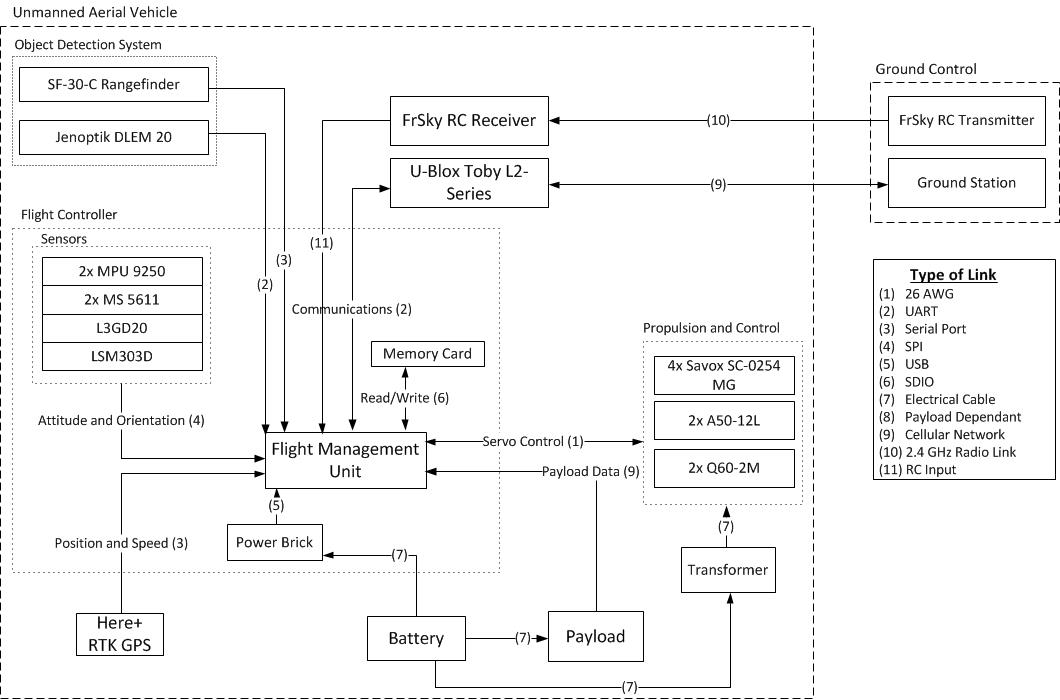
\includegraphics[width=.7\textwidth]{./CommandDataHandling/Figures/HWdiagram.jpg}
    \caption{Hardware Block Diagram}
    \label{fig:hwdia}
\end{figure}

\begin{figure}[ht]
    \centering
    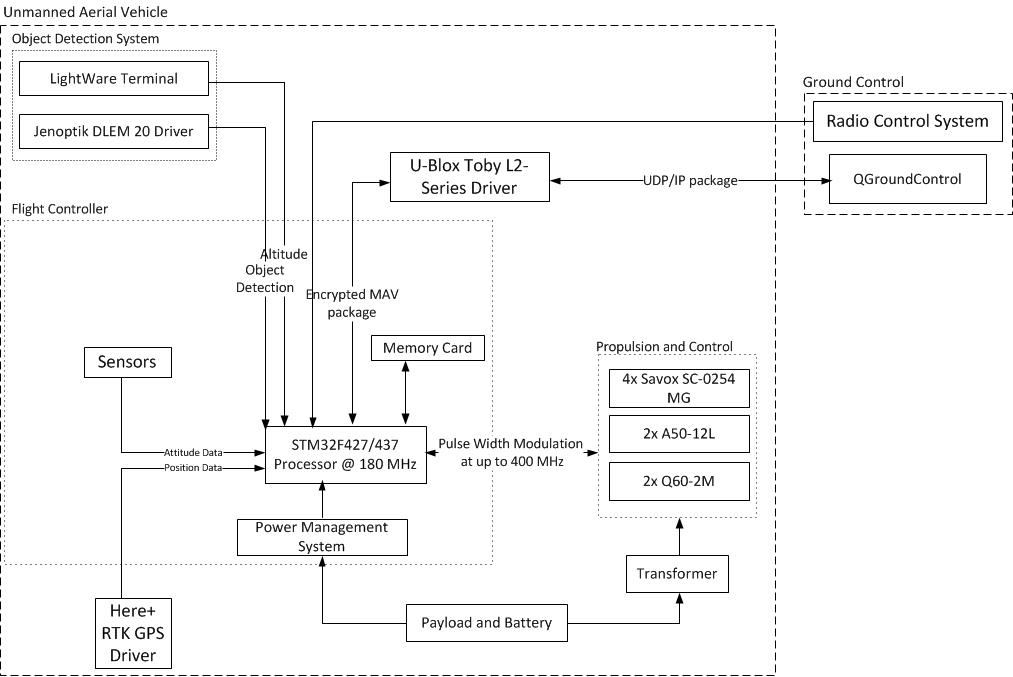
\includegraphics[width=.7\textwidth]{./CommandDataHandling/Figures/SWdiagram.jpg}
    \caption{Software Block Diagram}
    \label{fig:swdia}
\end{figure}

As seen in both diagrams, the central part of the system is the flight management unit. It is the processor used for autonomous flight control and to handle the data inside the system. With the exception of the propulsion and control system, all internal interfaces are connected to it and powered by it. Power related aspects are managed by the power brick. It regulates the voltage and current in order to prevent damage like burnout. It also monitors the power consumption and sends battery specific data to the flight management unit. 
The propulsion and control system in turn is powered by the battery itself. Each engine however has a separate transformer in order to reduce the battery voltage to its operational voltage. The figures show that the engines, actuators and servos used for propulsion and control use a 26 AWG link with PWM technique. The pixhawk 2.1 flight controller has 14 different PWM outputs, eight of them directly controllable by the R/C without need of the flight measurement unit. These will be the four engines used for thrust and the 4 servos used for control. The four tilting actuators are connected via the flight measurement unit. Finally, two more outputs are available in case the droppable payload module is connected for example. 

\section{Electrical Block Diagram}
\label{sec:elec_bloc_diag}



\autoref{fig:elec_diag} shows the electrical block diagram of the UAV system. It includes the different batteries used for power provision, buck converters to regulate the voltage and the different power receivers. Also the cable connectors required for disassembly and assembly are illustrated. As can be seen, the flight controller is just represented as one, more precise information regarding the internal structure can be found in the hardware diagram (\autoref{fig:hwdia}) or the pixhawk 2.1 datasheet \footnote{\url{http://www.unmannedtech.co.uk/uploads/6/7/0/2/6702064/pixhawk_2_25th_july_2016__2_.pdf}, Accessed 21-06-2017}. It was also decided to add two lights to the wing tips in order to make the drone visible in bad conditions. These will adhere to the conventional aircraft colours and hence use a red light on the left side and a green on the right side in order to make it possible to directly recognise the drones flying direction.

Considering the cabling of the system, there are several things that have to be considered during mounting. Firstly, the GPS module is located above the payload in order to receive best satellite signal. Also RC receiver and LTE module will be located here. Then, the flight controller and the other avionics are located in the nose of the fuselage, cabling to this part of the avionics will be minimal in order to avoid electromagnetic interference with the attitude sensors. Then, connections to the wing tips are needed for ailleron control, lights and speed sensor. The fuselage has an empty section above the payload department, which makes it possible to route cables through here. Then, through the wing, the cables can be routed through the shallow carbon tube. 
\begin{figure}[htb]
    \centering
    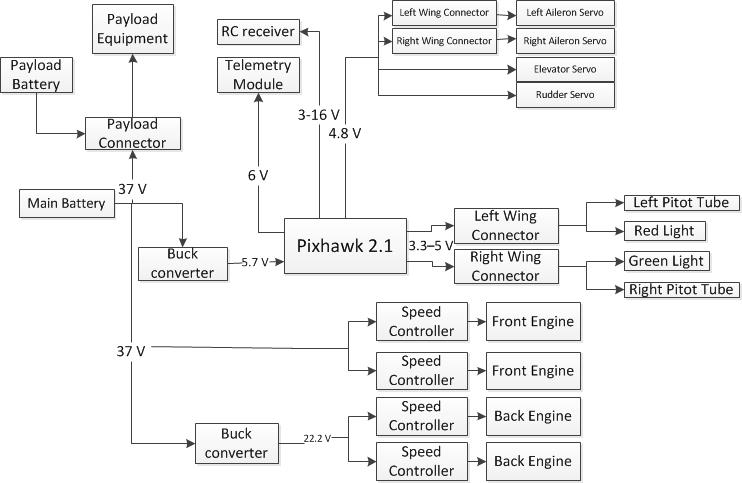
\includegraphics[width=.7\textwidth]{./CommandDataHandling/Figures/elecdiag.jpg}
    \caption{Electrical Block Diagram}
    \label{fig:elec_diag}
\end{figure}



    \chapter{Design Specifications}
\setlength{\parindent}{15pt}
\label{ch:desi_spec}

\section{Layout \& Configuration}
\label{sec:layo_conf}

\section{Performance Analysis}
\label{sec:perf_anal}

\section{Final Results}
\label{sec:fina_resu}

\section{Compliance Matrix}
\label{sec:comp_matr}

    \chapter{Operations \& Logistics}
\setlength{\parindent}{15pt}
\label{ch:oper_logi}

\section{Operations \& Logistics Concept Description}
\label{sec:oper_logi_conc_desc}

\begin{figure}[htb]
    \centering
    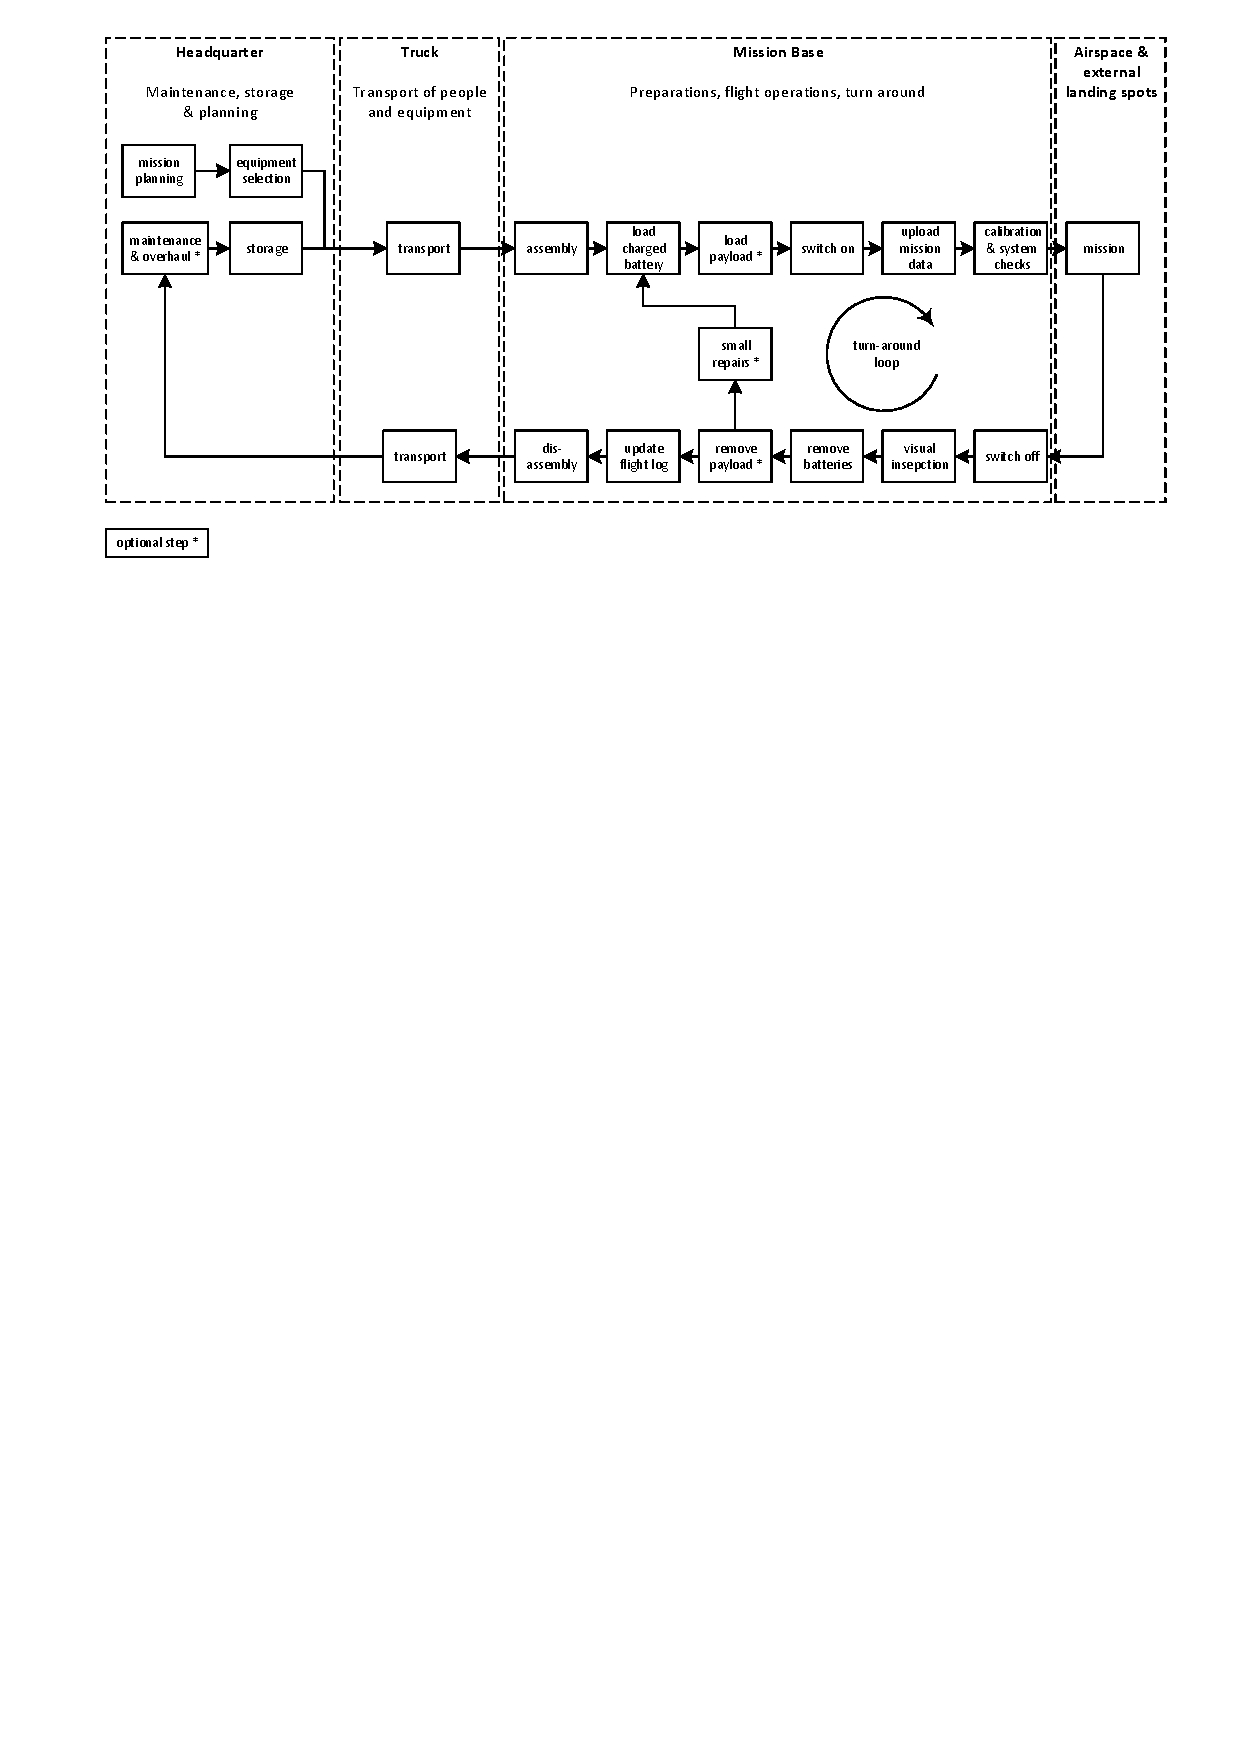
\includegraphics[width=1\textwidth]{OperationsLogistics/Figures/operations_logistics.pdf}
    \caption{Operations \& Logistics Flow Diagram}
    \label{fig:opslogsdig}
\end{figure}

\autoref{fig:opslogsdig} shows the the operations and logistics flow diagram for what this group expects to be typical operating conditions. It is assumed that the UAV operator has a main facility, from which the UAV, staff and mission relevant equipment are transported to a mission base at which flight operations take place. Naturally, variations to this scheme are possible, e.g. a parcel company may exclusively operate from its main facility, or long-range missions require a turn-around at a remote location, but for the sake of brevity only the most general case is presented.
The starting and end point of each mission is the so-called headquarters, the place where maintenance and storage takes place. Based on customer input a mission plan is set up, which determines the kind of resources that are required. Next to one or more UAVs, this includes staff on site, equipment such as the ground station, spare parts, additional batteries and a transport vehicle. Once the preparation is done, everything is loaded into a vehicle and transported to the location where the UAV is intended to take off and land. \autoref{fig:transport} shows the UAV body in disassembled state within a standard size van, where the remaining space can be filled with support equipment.
Once on site, the equipment needs to be unloaded and the UAV assembled into its operational form. A charged battery is then loaded, followed by the payload, which can also consist of another set of batteries. The system is switched on, the mission relevant data is uploaded to the on-board computer and an automated instrument calibration and readiness check performed. The UAV is now ready to fly and carry out its mission. After its return, the system is switched off for safety reasons, visually inspected and stripped off its batteries. The next steps depend on the kind of mission in question. If another flight is scheduled, the payload can be replaced and minor repairs taken out, e.g. replacing a damaged propeller blade. Once the battery is recharged or replaced by a full one, a new flight cycle can start. In case the mission does not comprise a turn-around or substantial damage was detected, the digital flight log is updated and the UAV disassembled. After loading all equipment the transport back to the headquarter takes place, where scheduled maintenance and all levels of repairs are carried out. Once the work is documented and approved, the equipment is stored and ready for the next mission.

\begin{figure}[htb]
    \centering
    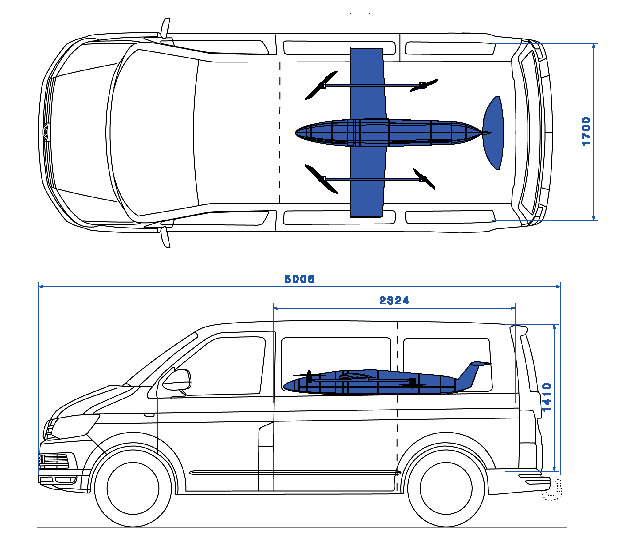
\includegraphics[width=0.7\textwidth]{OperationsLogistics/Figures/storage.pdf}
    \caption{UAV Van Transport}
    \label{fig:transport}
\end{figure}



\section{RAMS Characteristics} %chris somebody may write about maintainability if bored
\label{sec:rams_char}

In this section, the reliability, availability, maintainability and safety (RAMS) characteristics are presented. First, different safety critical functions are presented together with procedures to be carried out in their respective case. These procedures might include making use of a redundant system or emergency procedures to be carried out. The section concludes with a list of different maintenance activities. 
\nomenclature[A]{RAMS}{Reliability, Availability, Maintainability and Safety}

\subsection{Reliability and availability}

As explained in \autoref{ch:avio_grou_hand}, the UAV is highly dependant on the autopilot. Only for control in close range manual control is possible and even then the reliability of the flight controller, in order to manage the data flow, is of major importance. For this reason, the most critical functions are the ones needed for autonomous flight. The following paragraphs will explain one by one the failure of the different UAV components.

First, the flight controller bases all of its decision on the data it receives by the sensors. Wrongly assumed attitude or airspeed result in wrong actions and might in worst case lead to crashes. In order to prevent this from happening, redundancy is provided for the critical sensors. At least two accelerometers, barometers, magnetometer, gyroscopes and airspeed sensors are used in order to calculate attitude. The probability that all of them fail during a single mission can be assumed negligible. In case of object avoidance or ground distance sensor failure, the UAV will still be able to perform its mission, however the probability of crashing into an obstacle increases significantly and thus an emergency landing is performed. GPS data, with the help of pressure sensors will be used in order to determine a ground distance estimate during landing. GPS failure will result in the inability to determine the position and hence in mission failure. In this case also an emergency landing will be performed and a notification including last known position and failure reason will be send to the ground station. 

Another flight controller failure comes from the power source. Battery failure includes an empty battery, burnout or overvoltage. Empty battery will result in total failure, burnout and overvoltage can result in damaged hardware. In order to prevent this, the flight controller uses a power brick to manage the power supply. It sends useful information as battery status and battery level to the flight controller. This reduces the chances of wrong voltage distribution and makes it possible for the flight controller to perform a return to base procedure in case the energy level drops below a certain threshold. Regular inspection and replacement of the battery will also reduce the probability of battery failure. 

Then, servos are used throughout the system for either engine tilting mechanisms or control surface deflection. In the former, either one or more engines are stuck in horizontal or vertical position. In case only one or two engines are stuck, the remaining ones can be used to fly the drone to a safe location and perform a landing. If stuck in horizontal mode however, a safe vertical landing will not be possible anymore and a horizontal landing has to be performed. The impact of tilting actuator failure is minimal, as horizontal flight is still possible using only one engine. If actuators are stuck in vertical mode, a safe vertical landing can be performed. A more critical case is failure of a control surface. Aileron failure results in an inability to perform rolling action. This can be counteracted by the rudder and slight tilting of the engines. Rudder failure is counteracted using different thrust at each side and elevator failure is compensated for by tilting the front or back engines. Although redundancy is provided for control surface failure, a return to base procedure will be carried out in such a case to diminish the risk of further damage. 

After that, engine failure is a critical risk that has to be considered. One engine failure can be compensated by the rudder in horizontal flight, however vertical flight will not be possible anymore. In this case, also the forward propellers are used in order to generate enough thrust to perform a return to base procedure. Then in case of more engine failures, horizontal flight will be performed using the remaining engines and depending on the distance towards the base a new landing location might have to be chosen. In case the engines fail during vertical flight, no other option but to perform a emergency landing. This will not be possible in all cases but the flight controller will try to minimise the landing impact. 

The last failure to be considered is the failure of the telemetry link and the RC link. In this former case, no more waypoints can be send to the drone and the drone can not send updates regarding its flight conditions. If both links become unavailable, the drone will perform a return to base action resulting in mission failure. In order to minimise the risk of telemetry failure, missions always have to be planned and configured before UAV take-off. This makes it possible for the drone to perform its initial planned mission in case something goes wrong with the return procedure during link failure. 

In conclusion, all the critical systems used in the UAV system either have redundancy in case of failure or a safe procedure that can be performed limiting the damage. The most critical failure is an engine failure during vertical flight. Here no other option can be performed but landing the drone vertically while trying to minimise the impact. The reliability of the chosen engines however is high as explained in \autoref{ch:powe_prop}. As on top of that, the drone spends most of its mission time in horizontal flight, the probability of this event to occur is minimal. The modular design of the UAV ensures the availability of the drone, as in case of a failure, only the specific parts have to be exchanged. This can be performed without major complications. 

\subsection{Maintenance}

Next to the reliability aspect, availability and safety aspects strongly depend on the necessary maintenance procedures for the UAV. Extra maintenance will results in better safety aspects however, the availability will decrease. In case no maintenance is performed, the safety of the UAV can not be ensured anymore and if there is an unexpected failure the UAV will be unavailable for a longer period. The following shows different maintainability procedures depending on how often they have to be carried out. 
\newline


\paragraph{Start of mission}     \begin{enumerate}
    \item Check previous error log for previous mission problems and ensure that they have been fixed. 
    \item Make sure that battery is disconnected. 
    \item Assemble wing to fuselage.
    \item Inspect all connectors, propeller blades and wings for cracks. If cracks are present they have to be reported and maintenance might be necessary depending on the crack length and thickness. 
    \item Mount payload and connect a full battery.
    \item Establish cellular connection from UAV to ground station.
    \item Configure all waypoints needed for mission. 
    \item Control correct functioning of servos and engines using RC link. If an error occurs in the functioning it has to be reported and the mission will be aborted.
    \item Check correct calibration of sensors.
\end{enumerate}

\paragraph{End of mission} 
\begin{enumerate}
    \item Check internal error log for probable errors. If errors are present report them. 
    \item Disconnect battery and connect it to charger.
    \item Quick inspection on damages that might have occurred during mission.
    \item Disassemble wing from fuselage and clean different parts.
\end{enumerate}

\paragraph{Monthly Basis}
\begin{enumerate}
    \item Check all internal software for system updates and update them if necessary. 
    \item Full external inspection for cracks.
    \item Recalibration of all sensors.
\end{enumerate}























    \chapter{Production}
\setlength{\parindent}{15pt}
\label{ch:prod}
    \chapter{Life Cycle Assessment} 
\setlength{\parindent}{15pt}
\label{ch:susdevlca}

Sustainability is an import aspect of a design, as its principle of using minimal amount of material and energy is beneficial economically. This chapter elaborates on how sustainable development is incorporated in the design, followed by its LCA to see environmental impacts of the Hybrid UAV. 

\section{Sustainable Development}

Sustainability was mainly considered as a trade-off criterion in the midterm phase, however, its impact on design choices in the final phase is minimal due to high performance requirements as well as VTOL capabilities. 

%not sure about this, we really didn't give a shit about the sustainability. could someone have a look and add some to this?


\section{Life Cycle Assessment}

The technical framework for LCA can be seen in \autoref{fig:lcatriangle}. It starts with the central block, `Goal and Scope', then flows into Impact Assessment, Improvement Assessment and Inventory Analysis \cite{lca}.

\begin{figure}[H]
    \centering
    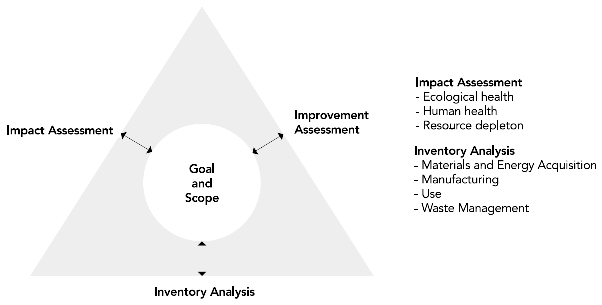
\includegraphics[width=0.8\textwidth]{LifeCycleAssessment/Figures/LCAtriangle.pdf}
    \caption{Technical Framework for Life Cycle Assessment}
    \label{fig:lcatriangle}
\end{figure}

\subsection{Goal and Scope}
The goal and scope definitions need to be determined as a first process of a LCA. The following paragraphs elaborate on details of each aspect of the first process. 

\paragraph{Goal} The MNS can be used to define the goal. The MNS states, `Carry out both supervised and autonomous monitoring and transport missions, comprising vertical take-off and landing, and high-velocity in horizontal flight.' %is this correct?

\paragraph{Scope} In order to define the assessment methods, a system to be studied and system boundaries need to be determined. Functions of the system have been identified based on a functional breakdown structure in the baseline report \cite{baseline}, and can be summarised into three categories as following: 

\begin{itemize}
    \item Perform air transport
    \item Perform various missions
    \item Perform missions under various conditions
\end{itemize}

\paragraph{Functional Unit}
A main purpose for a functional unit is to set a normalised basis of comparison. For a consistent analysis, it is decided that further quantitative comparison will have a normalised scale from 0 to 100.

\paragraph{System Boundaries}
System boundaries are defined based on requirements, which can be found in \autoref{ch:syst_desc}.

\paragraph{Data Quality}
Data quality in LCA is reflected in the final LCA. At this point of the stage, it is not possible to come up with a consistent and traceable data quality, such as time-related coverage, geographical coverage and technological coverage \cite{lca}. It will be established in the next phase of the project. 

\paragraph{Critical Review Process}
Critical review process is not applicable, since the process is mainly for certification of a system or product and publication of the project in terms of environmental standards.

\subsection{Inventory Analysis} 
Inventory analysis is carried out after defining goal and scope definition. The online U.S Life Cycle Inventory Database\footnote{\url{https://uslci.lcacommons.gov/uslci/search}} and the offline version \cite{USLCI} are used to determine specifications of 3 different phases that are shown in \autoref{fig:lcawheel} as following: product manufacturing, use, end of life. The analysed items adhere to the production plan, which can be found in \autoref{ch:prod_plan}. Each Life Cycle Inventory (LCI) data is directly taken from the U.S Life Cycle Inventory Database. The inventory analysis primarily uses $CO_{2}$ footprint and Cumulative Energy Demand (CED).

\nomenclature[A]{CED}{Cumulative Energy Demand}

\paragraph{Assumptions} There are several assumptions used for LCI.
\begin{itemize}
    \item For E-glass composites, the ratio of E-glass and high density polyethylene resin is 1:1.
    \item Carbon fibre composites are mainly made from acrylonitrile copolymer.
    \item Possible choices for different production methods are eliminated and assume that environmental impacts of all manufactured components do not differ in terms of different production methods.
    \item Batteries are recharged by a natural gas powerplant in the Netherlands.
\end{itemize}

\nomenclature{LCI}{Life Cycle Inventory}

\begin{figure}[H]
    \centering
    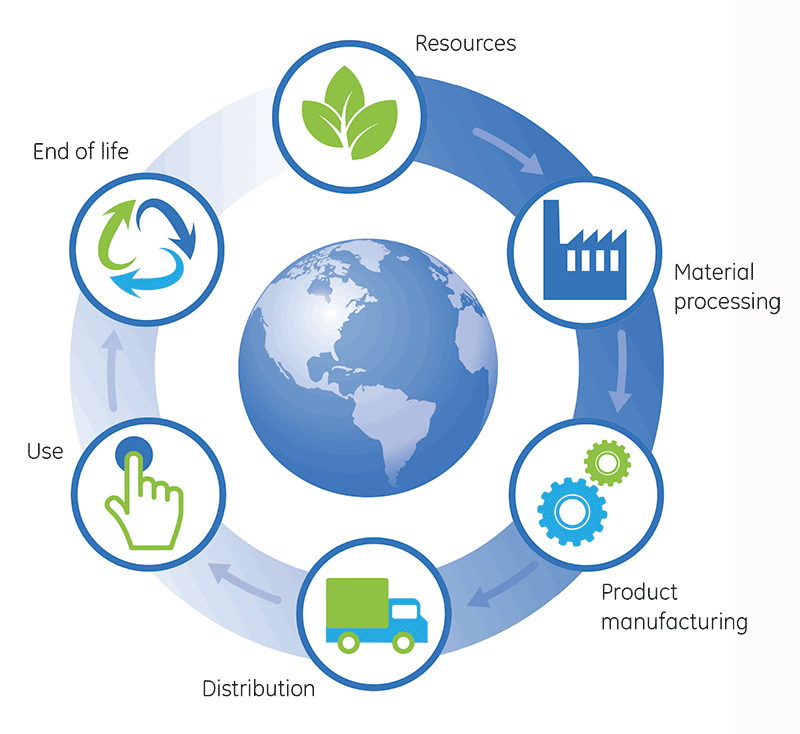
\includegraphics[width=0.5\textwidth]{LifeCycleAssessment/Figures/lcadiagram.jpg}
    \caption{Life Cycle Assessment Wheel}
    \label{fig:lcawheel}
\end{figure}

\paragraph{Materials \& Energy Acquisition and Manufacturing Phase} This section analyses $CO_{2}$ footprint and CED for manufactured components, as purchased components are not considered for materials \& energy acquisition and manufacturing phase.\\
For the fuselage, E-glass and high density polyethylene resin are used. To produce the fuselage, 3.633 kg of $CO_{2}$ is emitted and 201.9 MJ of CED is needed, which can be seen in \autoref{tab:eglasscomp}

\begin{table}[H]
\centering
\caption{Fuselage Production LCI}
\label{tab:eglasscomp}
    \begin{tabular}{lcc}
    \toprule
    Material per kilogram         &$ CO_{2}$ footprint [kg] & CED [MJ]  \\\midrule
    E-glass                         & 0.141                & 4.572    \\\hdashline
    High density polyethylene resin & 1.312                & 76.20    \\\hline \hline
    \textbf{Fuselage total (2.5 kg)}                 & \textbf{3.633}                & \textbf{201.9}   \\\bottomrule
    \end{tabular}
\end{table}

A carbon fibre rod and Expanded Polypropylene (EPP) foam are used to produce the wing. Most carbon fibre composites are made from polyacrylonitrile as their base\footnote{\url{http://www.compositesworld.com/blog/post/the-making-of-carbon-fiber}, Acessed on 26-06-2017}. The LCI of the wing can be seen in \autoref{tab:winglci}. In order to produce the wing, 5.642 kg of $CO_{2}$ is emitted and 217.8 MJ of CED is needed.

\nomenclature[A]{EPP}{Expanded Polypropylene}

\begin{table}[H]
\centering
\caption{Wing Production LCI}
\label{tab:winglci}
    \begin{tabular}{lcc}
    \toprule
    Material per kilogram       & $CO_{2}$ footprint [kg] & CED [MJ] \\\midrule
    Acrylonitrile copolymer     & 3.134                & 105.3    \\\hdashline
    Polypropylene resin for EPP & 1.216                & 75.20    \\\hline
    Carbon fibre rod (0.588 kg)       &  1.843                    &  61.92        \\\hdashline
    Carbon fibre ribs (0.893 kg)      &   2.799                  &  94.03           \\\hdashline
    EPP foam (0.822 kg)         &   1.000                   &  61.81        \\\hline \hline
    \textbf{Wing total (2.500 kg)}   & \textbf{5.646}                     & \textbf{217.8}              \\\bottomrule
    \end{tabular}
\end{table}

For painting the UAV, a method of simple top coat is chosen. Per square meter of surface area, 0.731 kg of $CO_{2}$ is emitted and CED of  10.24 MJ is required. The total surface area of the UAV and corresponding $CO_{2}$ \& CED values can be seen in \autoref{tab:painting}. The surface area of the wing, the horizontal stabiliser and the vertical tail are multiplied by 2, as both sides of each component have to be painted. 3.056 kg of $CO_{2}$ is emitted and 31.29 MJ of CED is required in order to paint the UAV.

\begin{table}[H]
\centering
\caption{UAV Painting LCI}
\label{tab:painting}
    \begin{tabular}{lccc}
    \toprule
                          & Surface area [$m^2$] & $CO_{2}$ footprint [kg] & CED [MJ] \\\midrule
    Automotive painting (top coat) & 1  &   0.7310 & 10.24 \\\hline
    Fuselage              & 1.184                    & 0.8655                 & 12.12    \\\hdashline
    Wing                  & $0.8010\cdot2$                 & 1.171                  & 16.40    \\\hdashline
    Horizontal stabiliser & $0.1062\cdot2$                 & 0.1553                 & 2.175    \\\hdashline
    Vertical tail         & $0.02893\cdot2$                & 0.04230                & 0.5925   \\\hline \hline
    \textbf{UAV total}             & \textbf{3.056}                    & \textbf{2.234}                  & \textbf{31.29}    \\\bottomrule
    \end{tabular}
\end{table}

For transporting manufactured parts, a diesel-powered combination truck is used. Per km of transport, the truck emits 0.0799 kg of $CO_{2}$. However, distance between a factory and an assembly facility is not defined, thus the transport $CO_{2}$ footprint will not be considered for analysis.

\paragraph{Use Phase}
%something about transport and battery-charging
During the use phase, batteries have to be charged per mission. Per GJ of heat generated by a natural gas powerplant, it emits 56 kg of $CO_{2}$\cite{USLCI}. In order to transfer the heat to electricity, an efficiency of 39 \% is taken \cite{electricity}. Thus, 56 kg of $CO_{2}$ is emitted from generating 0.39 GJ of electricity. Using the battery capacity of 24190 mAh as the most extreme flight scenario, required power can be found to be 467 W, based on \autoref{eq:battcap} and P = I*V. Defining that the flight time for the most extreme flight scenario is 115 minutes according to \autoref{tab:extreme}. By multiplying the required power with time, which is $467\cdot115\cdot60$, the required energy is 3.222 MJ per the most extreme flight scenario mission. The requirement SYS-OP-2.1 states that the UAV shall have an operational life of at least 1500 flying hours. By dividing 1500 flying hours with 115 minutes of each mission, 783 missions can be launched. Thus, $3.222\cdot783$ MJ of energy is needed to recharge batteries for 783 missions, which translates to 2.523 GJ of electricity. By dividing the required electricity with the unit electricity of 0.39 GJ and multiplying it by the unit $CO_{2}$ footprint of 56 kg, 362.3 kg of $CO_{2}$ is emitted for 1500 flying hours. 

\paragraph{Waste Management}
EPP can be fully recycled into new wing parts, while carbon fibre rods and ribs cannot be recycled into new parts due to undesirable reduction in mechanical properties. Thus, the carbon fibre parts are considered as waste to be left in deposit containers at collection points. $CO_{2}$ footprint of the disposal method is 0.040 kg and CED of 0.55 MJ is required.\\
Disposal of lipo batteries is landfill safe, if they are processed with a salt water method, which discharges the batteries slowly and completely as well as neutralises the lithium. Thus, no carbon footprint and CED are considered for disposing lipo batteries.\\
Raw materials such as gold, silver, palladium and platinum are first extracted from circuit boards then metal parts such as steel and aluminium are removed. Then the plain circuit boards are chopped and recycled into different products or new circuit boards. Thus, no carbon footprint and CED are considered here.

\subsection{Impact Analysis}
Impact analysis is left for future as data regarding the following cannot be found without a proper license to access to detailed online database: abiotic resources, biotic resources, land use, global warming, stratospheric ozone depletion, ecotoxicological impacts, human toxicological impacts, photochemical oxidant formation, acidifitcation, eutrophication and work environment.


\subsection{Interpretation}
With the complete inventory analysis, it is possible to identity hot-spots of the UAV in terms of $CO_{2}$ footprint and CED. \autoref{tab:hotspot} shows carbon footprint and CED for different elements analysed for LCI. Recharging batteries for 1500 flight hours emits the most $CO_{2}$ of 362.3 kg and requires the highest CED of 2523 MJ. Thus, recharging batteries during the use phase is the hot-spot.


\begin{table}[H]
\centering
\caption{Hot-Spot Identification for LCI}
    \label{tab:hotspot}
    \begin{tabular}{l|cc}
    \toprule
                                           & $CO_{2}$ emission [kg]        & CED [MJ]                     \\\hdashline
    Fuselage production                    & 3.633                         & 201.9                        \\\hdashline
    Wing production                        & 5.646                         & 217.8                        \\\hdashline
    UAV painting                           & 2.234                         & 31.29                        \\\hdashline
    Battery recharge (1500 flight hours) & \cellcolor[HTML]{FE0000}362.3 & \cellcolor[HTML]{FE0000}2523 \\\hdashline
    Part disposal                          & 0.040                         & 0.550   \\\bottomrule                    
    \end{tabular}
\end{table}

As a recommendation, different types of propulsion systems should be considered for future, such as a hybrid propulsion, an internal combustion propulsion or electric propulsion powered by renewable energy. 





    %Conclusion
    \chapter{Conclusion \& Recommendations}
\setlength{\parindent}{15pt}
\label{ch:conc_reco}

%purpose of report, also quickly summarise previous (20 conc)
The aim of this report is to document the continuation of the design process and to justify the choices that were made in the preliminary design phase. The concept used, the Winged Quadcopter, was determined in the midterm report \cite{midterm}. It was considered best after a trade-off between five options, as brought forward in the baseline report \cite{baseline}. The goal of the final design is to adhere to the mission need statement:
\begin{quote}
\itshape `Carry out both remotely controlled and supervised autonomous monitoring and transport missions, comprising vertical take-off and landing, and sustained high-velocity horizontal flight.'
\end{quote}

The design was carried out by five specialist teams, resulting in a concurrent engineering structure where design parameters are constantly updated after each design stage. These teams are aerodynamics, structure, command and data handling, power \& propulsion and stability \& control. Each had their corresponding tasks, and were the responsible team for these.

To start off the designing, a trade-off between five preliminary concepts was performed in order to determine what type of Hybrid UAV layout is optimal for the given requirements. The most important requirements are top speed of 200 km/h, endurance of at least an hour, a payload carrying capacity of 10 kg and a capability to take-off and land vertically. These requirements have been set by the client. However, it is determined that it is unfeasible to meet all these requirements simultaneously while adhering to the EASA mass limitation of 25 kg. To solve this, modular payloads are used, replacing payload weight with batteries if necessary. To prevent exceeding limits on mass, cost, and power, budgets have been implemented for each subsystem. To have an allowable margin of freedom, contingencies have been added to each budget. Subsystems were not allowed to exceed these budgets, if this was the case, changes had to be made to the design or budget. 


With the preparation done, the five departments worked concurrently on the various subsystems to design the most optimal outcome. Using a master set document with all updated variables, each department worked with the most up-to-date values. The final outcome resulted in a design that even exceeds some of the requirements. The aircraft is able to fly 40 km with a full payload, while being able to fly up to a maximum of 600 km by replacing payload weight with extra batteries. The requirement of having an endurance for an hour has been met, but not with the full payload capacity. The structure of the aircraft will be built with lightweight materials such as glass fibre and carbon fibre to ensure the mass of the aircraft will not exceed 25 kg. To conclude, the design meets the requirements using a modular payload, while staying within the budgets assigned to the subsystems.


\paragraph{Recommendations} With the preliminary design, the overall layout and approximate parameters are known.  For future design stages, the team has some suggestions on things that can be improved. For example, the fuselage can be made shorter, decreasing drag. Besides that, in the current design a modular payload is used to optimise performance per mission type. In the future, modularity can also be applied to the wings, props and engines. Also, more extensive CFD analysis should be done to enhance the aerodynamic design. Stability should be investigated more thoroughly, including dynamic stability properties. Finally, when more Hybrid UAVs are sold, some components that are currently off-the-shelf, such as the flight control module, can be replaced by in-house designed ones.


    
    
    %References:
    \begingroup %Creates Separate Group from the Report
    \raggedright %Removes Justification
    %\nocite{*} %Disables biblatex from checking if all references are cited in-text DO NOT UN-COMMENT UNLESS ERROR CHECKING!
    \cleardoublepage
    \phantomsection
    \addcontentsline{toc}{chapter}{\BibliographyName}
    \printbibliography[title={\BibliographyName}] %Rename Bibliography (Default) to \BiblographyName defined in style.cls
    \endgroup

    
    %Appendices:
    \begin{appendices}
    \chapter{Full List of Requirements}
\setlength{\parindent}{15pt}
\label{ch:full_list_requ}


    \end{appendices}
\endgroup
\end{document}